\documentclass[12pt,twoside]{report}
\usepackage[utf8]{inputenc}
\usepackage{graphicx}
\graphicspath{{images/}}
\usepackage{float}
\usepackage{caption}
\usepackage{subcaption}
\usepackage[a4paper,width=150mm,top=25mm,bindingoffset=6mm]{geometry}
\usepackage{fancyhdr}
%\pagestyle{fancy}
%\fancyhead{}
%\fancyhead[RO,LE]%{\chaptername}
%\fancyfoot{}
%\fancyfoot[LE,RO]{\thepage}
%\fancyfoot[LO,CE]{Chapter \thechapter} %leftmark or \rightmark
%\fancyfoot[CO,RE]{Willi Carlsen}
\renewcommand{\headrulewidth}{0.4pt}
\renewcommand{\footrulewidth}{0.4pt}

\usepackage[backend=biber]{biblatex} %style=authoryear
\addbibresource{references.bib}
\usepackage{hyperref}

\usepackage{amsmath}
\usepackage{amssymb}

\usepackage{siunitx}

\usepackage[version=3]{mhchem}

\usepackage{booktabs}

\title{
    {Cryogenic cavity optomechanics with ultrahigh-Q membrane resonators}\\
    {\large Niels Bohr Institute}\\
    {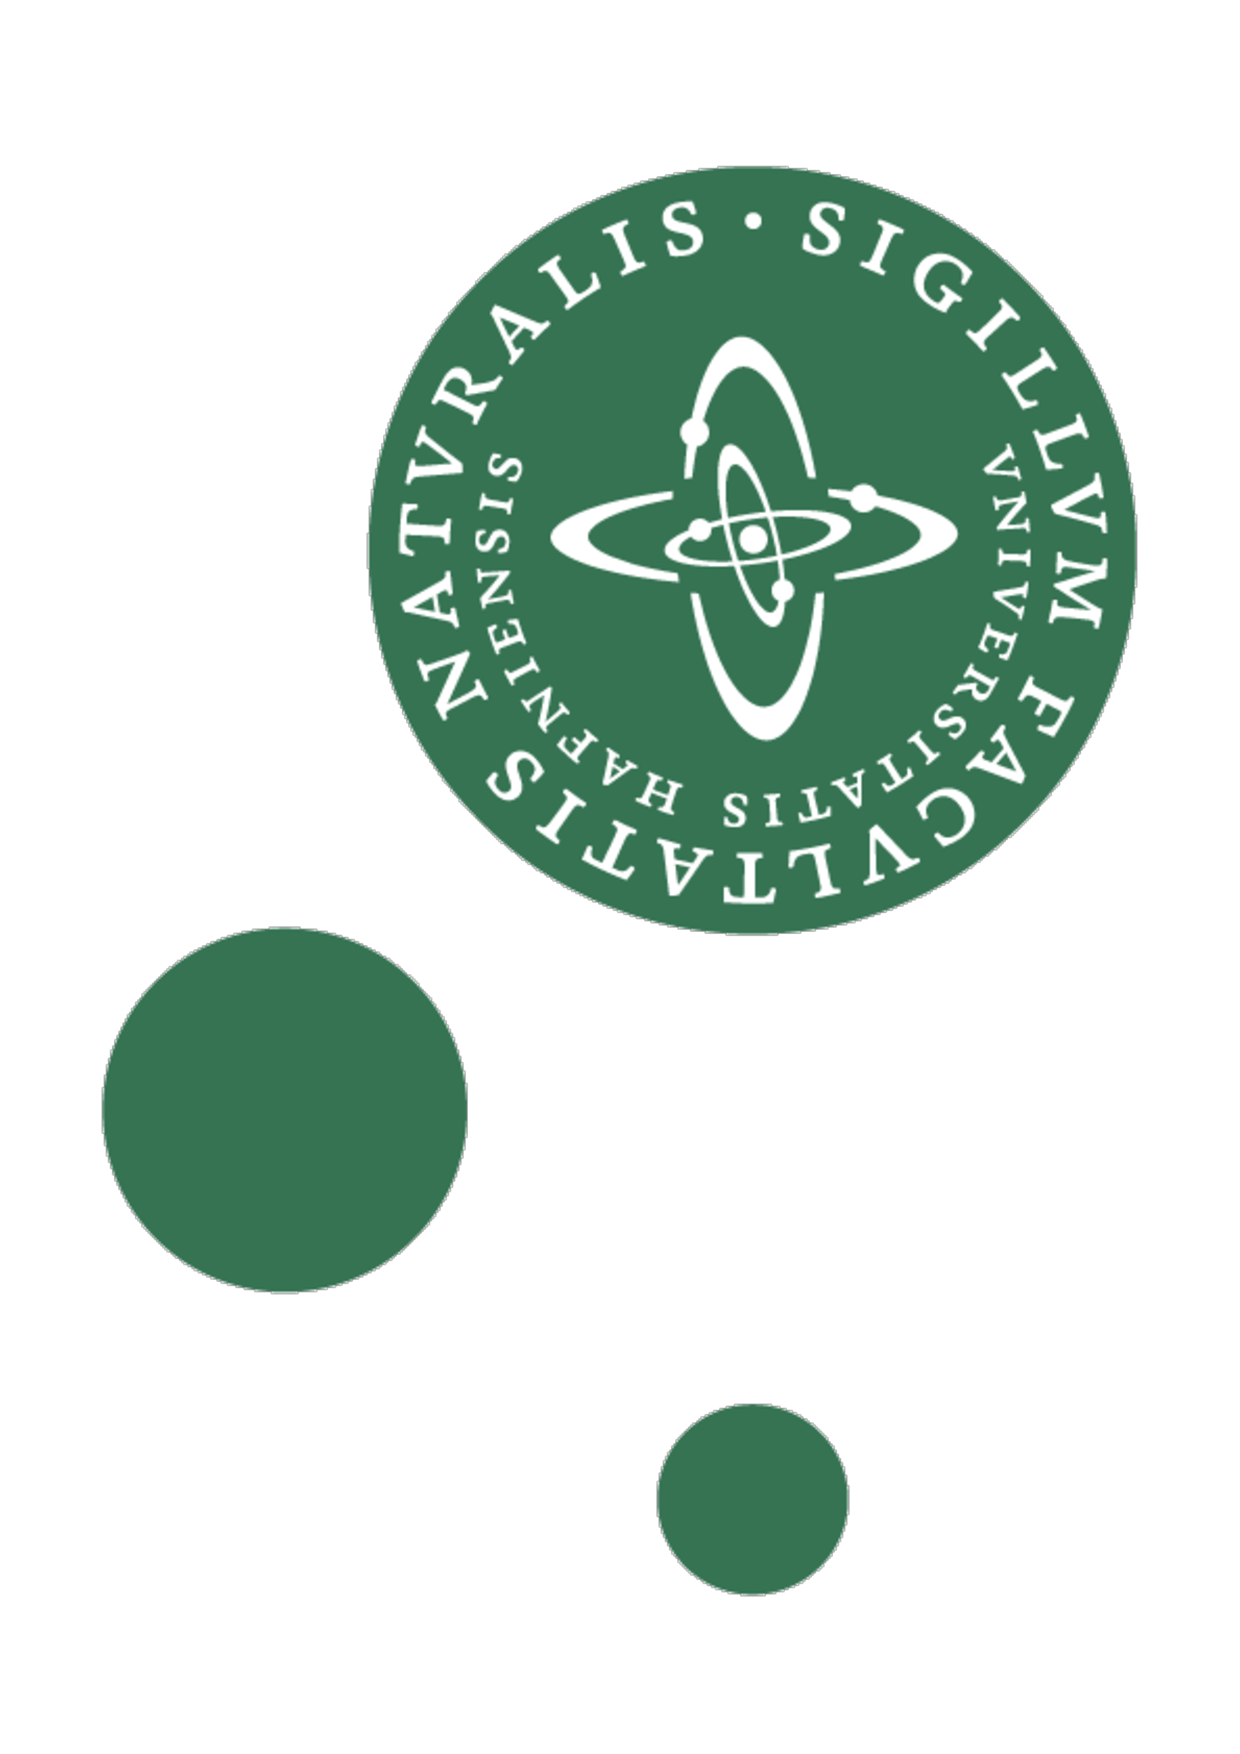
\includegraphics[scale=0.25]{uni_logo.pdf}}
}
\author{Willi Carlsen\\ \\
Supervisor: Eugene S. Polzik}
\date{August 2015}

\begin{document}

\maketitle

\chapter*{Abstract}
During the past years we have set up an optomechanical membrane-in-the-middle system towards showing a quantum enabled system, by squeezing of light or cooling a nanomechanical resonator to its motional ground state. The work presented here describes our efforts towards ground state cooling.

The setup consist of a high finesse optical Fabry-Perot cavity with a highly stressed silicon nitride nanomechanical resonator placed inside. The nanomechanical resonator is shielded from the environment by a phononic bandgap structure, but due to complications of low frequency modes of the collective structure, the sample is returned to the state of a regular nanomechanical resonator, i.e. by damping the bandgap structure within which the membrane is suspended. A sample holder is designed to achieve good thermalization of the nanomechanical resonator. The system is characterized at cryogenic temperatures in pursuit of optical sideband cooling of a mechanical mode to the ground state.

We have achieved a finesse of $\sim56\mathrm{k}$ (corrosponding to an optical linewidth of $\sim$\SI{1.6}{\mega\hertz}) with a high-Q ($\sim6\times10^6$) membrane embedded inside the optical cavity. The single photon coupling for the (3,3)-mode of the membrane is $\sim$\SI{88}{\hertz} (measure by means of optomechanical induced transparency) and the effective mechanical broadening achieved with the highest optical powers was measured to be $\sim$\SI{5.5}{\kilo\hertz}. As such, we were able to record a minimum phonon occupancy of $27\substack{+11 \\ -7}$, corresponding to an effective temperature of $\sim$\SI{3}{\milli\kelvin}.

\chapter*{Acknowledgment}
I would like to express my gratitude to everyone who took part in the process of this thesis and in the experiment in general. It has been a pleasure working with so many brilliant and dedicated individuals and I have enjoyed being part of the Quantop group at the Niels Bohr Institute for the past few years.
\\
\\
\noindent
A special thanks to:
\\
\noindent
Eugene Polzik for opening the door and letting me be a part of the Quantop group and for igniting my initial interest in quantum optics and optomechanics.
\\
\\
\noindent
Albert Schlie{\ss}er for always having his door open for discussions and providing much needed guidance even in moments of doubt.
\\
\\
\noindent
William Nielsen for being a brilliant mentor from the very beginning and towards the end being priceless in every possible way.
\\
\\
\noindent
Christoffer Moeller for many inspiring discussions and providing great long distance help.
\\
\\
\noindent
Yeghishe Tsaturyan for being my dear friend all the way through university and for carrying me across the finish line.
\\
\\
\noindent
Andreas Barg for always being ready to help out when needed and for being a great office buddy.
\\
\\
\noindent
Anders Simonsen for the late night advice while pulling an all-nighter.
\\
\\
\noindent
Jörg Müller for being Jörg. Every lab should have a Jörg.
\\
\\
\noindent
Stefan Christensen, Jean-Baptiste Benguin, Jürgen Appel, Anreas Naesby, Tolga Bagci, Rodrigo Thomas, Eva Bookjans, Koji Usami, Georgios Vasilakis, Heidi Soerensen, Kasper Jensen, Dennis Wistisen and of course the rest of the Quantop staff.

\tableofcontents

\chapter{Introduction}
Traditionally, we associate experiments in quantum mechanics with some of the smallest constituents of matter, such as atoms or ions. In resent years macroscopic objects have proven to be a promising testbed of quantum mechanics, due to significant advances within material science and fabrication. As a result, the field of optomechanics has sprung and gained considerable momentum in resent years. Among experiments in fundamental quantum optomechanics are ground state cooling of macroscopic mechanical object \cite{oconnell2010, chan2011, teufel2011}, squeezing of light in an optomechanical system \cite{purdy2013, safavi2013}, back-action evation \cite{suh2014} and many others.

Optomechanical systems come in many flavours and span from optomechanical crystals \cite{chan2011}, whispering-gallery-mode microresonators \cite{schliesser2009}, to superconducting circuits \cite{teufel2011, oconnell2010, suh2014} and nanomechanical resonators inside standard Fabry-Perot optical cavities \cite{jayich2008}. The system presented in this work belongs to the latter category and is commonly referred to as the {\it{membrane-in-the-middle}} system. The system was pioneered by the group of Jack Harris in 2008 \cite{jayich2008}. It combines one of the most studied type of optical cavities with one of the most promising mechanical resonators, namely highly stressed silicon nitride membranes, ensuring high optical, as well as mechanical, quality factors. Despite great progress towards the ground state, this goal has yet to be achieved for this particular system. The work present in this thesis describes the membrane-in-the-middle system at the Niels Bohr Institute and our quest for ground state cooling.

\chapter{Theory}

\section{Membrane resonators}

\subsection{Vibrational modes} \label{sec:vib_modes}
To understand the vibrational behavior of the nanomechanical resonator in our optomechanical system, we consider a simple model of a pre-stressed thin plate (two-dimensional). In our case it is  a square membrane with side lengths $l$ and thickness $h$. In the actual device the membrane is suspended on a rigid silicon frame along the sides, which mathematically implies fixed boundary conditions. The membrane only displaces out of plane with amplitude $w$ see figure \ref{fig:vib_mod_mathdef}.

\begin{figure}[h!]
\begin{center}
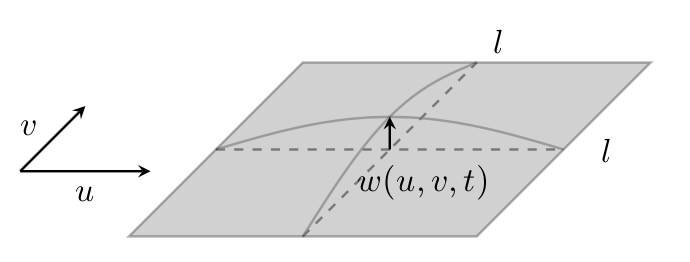
\includegraphics[scale=0.75]{vibrational_modes_mathdef.png}
\end{center}
\caption{Vibrating square nanomechanical membrane with fixed boundary conditions. The transverse (out-of-plane) displacement is denoted $w(u, v, t)$. The picture is lent from \cite{barg2014}.}
\label{fig:vib_mod_mathdef}
\end{figure}

If we assume $l \gg h$, i.e. corresponding to assuming a two-dimensional film, then the math simplifies significantly and we no longer have to consider different strains and stress distributions along the out-of-plane axis, i.e. in various depths of a bulk system. We describe the displacement $w(u, v, t)$ as a two-dimensional elastic wave equation \cite{Wilson2011}

\begin{equation}
\nabla^2 w = \frac{1}{C_s^2}\frac{\partial^2 w}{\partial t^2},
\label{eq:2dwave}
\end{equation}
\noindent
where $C_s$ is the wave propagation speed and $\nabla = \left(\frac{\partial}{\partial x_1},...,\frac{\partial}{\partial x_n} \right)$ is the nabla operator. By imposing the boundary conditions $w(u, 0, t) = w(0, v, t) = w(u, l, t) = w(l, v, t) = 0$ and using separation of variables, $w(u, v, t) = U(u)V(v)T(t)$ (assuming $U(u)V(v)T(t) \neq 0$), equation \eqref{eq:2dwave} takes the following form

\begin{equation}
\frac{1}{U}\frac{\partial^2 U}{\partial u^2} + \frac{1}{V}\frac{\partial^2 V}{\partial v^2} = \frac{1}{C_s^2}\frac{1}{T}\frac{\partial^2 T}{\partial t^2}
\label{eq:2dwavesep}.
\end{equation}
\noindent
Each term in this equation depends on different variables, therefore, each one of them must be equal to a constant. We recognize the textbook example of a simple harmonic oscillator, i.e. $\frac{1}{U}\frac{\partial^2 U}{\partial u^2} = -k_m^2$. The solution with regards to the boundary conditions is sinusoidal

\begin{subequations}
\begin{align}
U(u) & = U_0\sin(k_m u)\\
V(v) & = V_0\sin(k_n v)\\
T(t) & = A_{m,n}\cos(\Omega_{m,n} t) + B_{m,n}\sin(\Omega_{m,n} t),
\end{align}
\label{eq:modeshape}
\end{subequations}
\noindent
here $k_{m} = \frac{m\pi}{l}$ and $k_{n} = \frac{n\pi}{l}$, where $m,n \in \mathbb{N}$ specify the number of anti-nodes along the two directions. The angular eigenfrequencies $\Omega_{m,n}$ are given by the following dispersion relation \cite{wilson2009}

\begin{equation}
\Omega_{m,n} = \frac{C_s \pi}{l}\sqrt{m^2 + n^2} = \frac{\pi}{l}\sqrt{\frac{\tau}{\rho}}\sqrt{m^2 + n^2}\\
\label{eq:fundmode},
\end{equation}
\noindent
where $\tau$ is the in-plane tensile stress and $\rho$ the density. Of course the membrane could be asymmetric in stress or side length and the model could be extended to accommodate for asymmetry, but we will assume that this is not the case. If the fundamental angular eigenfrequency $\Omega_{1,1}$ is known, we can quickly calculate the higher order modes using $\Omega_{1,1}\sqrt{m^2 + n^2}/2$. We can estimate the fundamental eigenfrequency $f_{1,1} = \frac{\Omega_{1,1}}{2\pi}$ from typical membrane properties in table \ref{tab:memprop} using equation \eqref{eq:fundmode}. Note the relative size between the thickness and side length, which justifies our previous claim of $l \gg h$.

\begin{table}[H]
\centering
\begin{tabular}{ccc}
\toprule
$l$ & Side length  & \SI{540}{\micro\meter} \\
$h$ & Thickness & \SI{45}{\nano\meter} \\
$\rho$ & Density & \SI{2.3d3}{\kilogram\per\cubic\meter} \\
$\tau$ & Stress & \SI{1}{\giga\pascal} \\
\midrule
$f_{1, 1}$ & Eigenfrequency & \SI{732}{\kilo\hertz} \\
\bottomrule
\end{tabular}
\caption{Common membrane parameters and estimated fundamental eigenfrequency $f_{1,1}$. The picture is borrowed with permission from \cite{barg2014}.}
\label{tab:memprop}
\end{table}
\noindent
Futher more using equations \eqref{eq:modeshape} we can visualize the vibrational mode shape of the membrane for the different modes. We should keep in mind that ``real" vibrational motion is sum of all vibrational modes and not as simple as the presented for the isolated modes in figure \ref{fig:modeshape}.

\begin{figure}[H]
    \centering
    \begin{subfigure}[b]{0.49\textwidth}
        \centering
        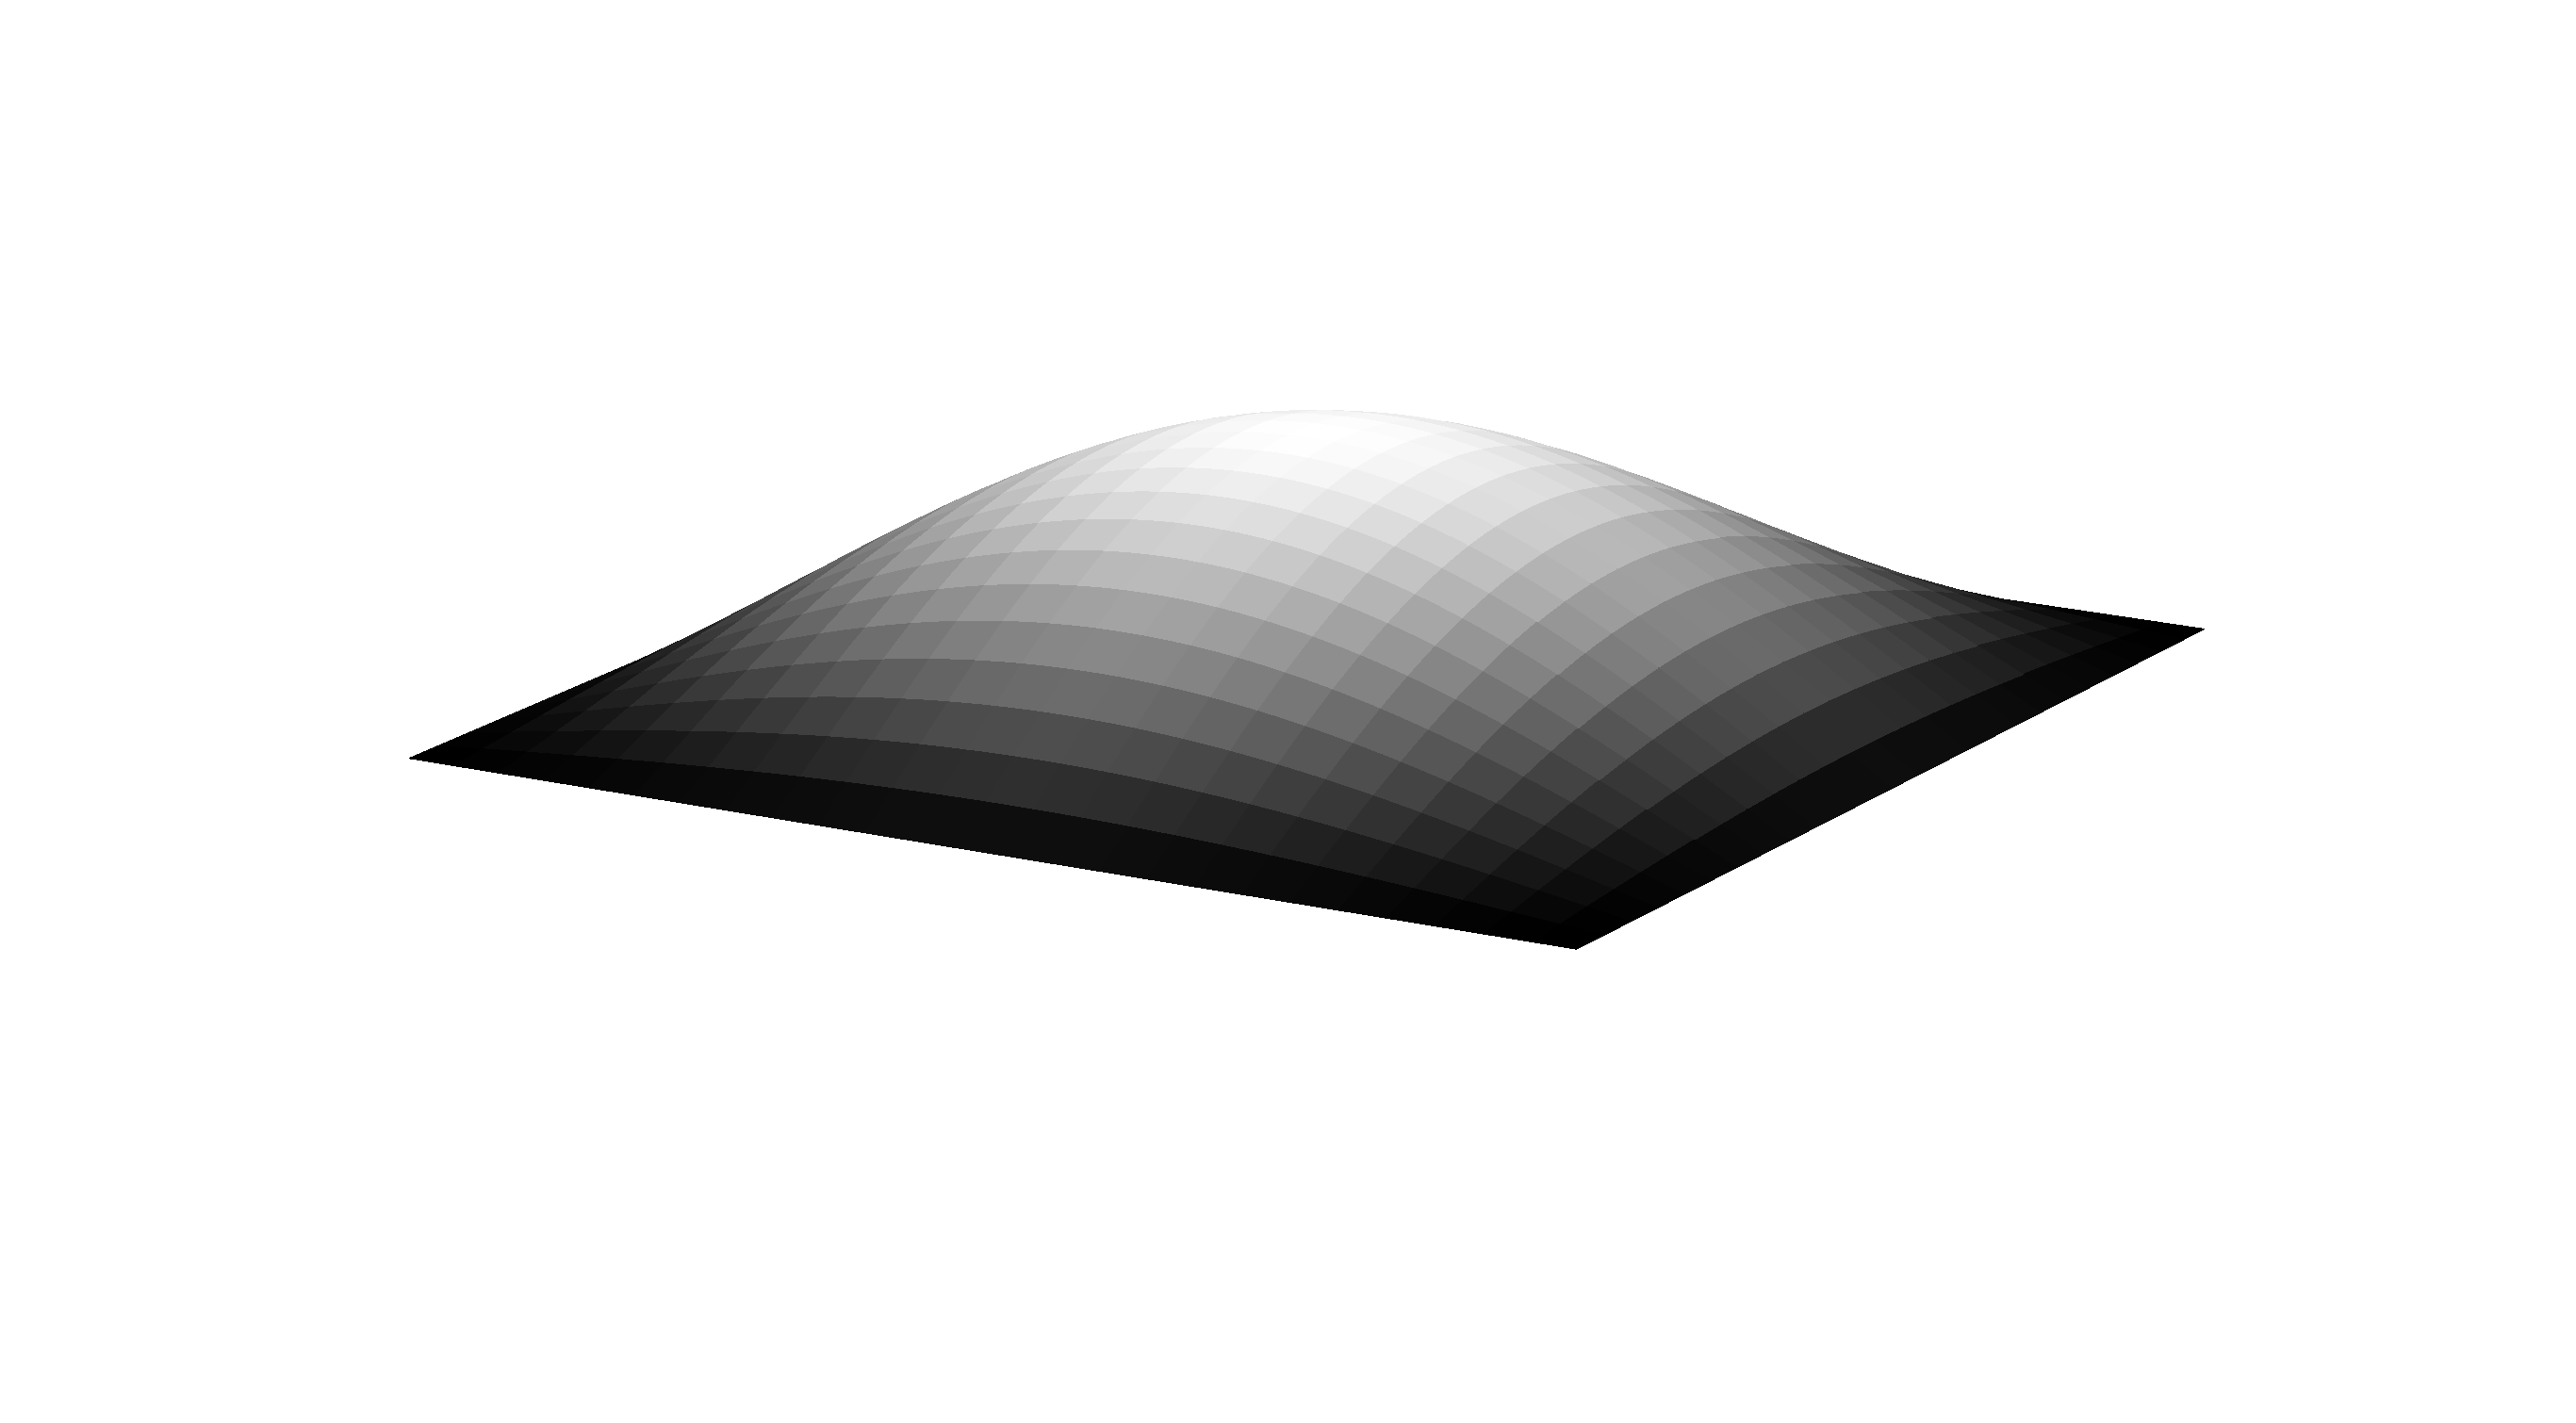
\includegraphics[width=\textwidth]{/modes/mode11.eps}
        \caption*{(1,1)}
    \end{subfigure}
    \hfil
    \begin{subfigure}[b]{0.49\textwidth}
        \centering
        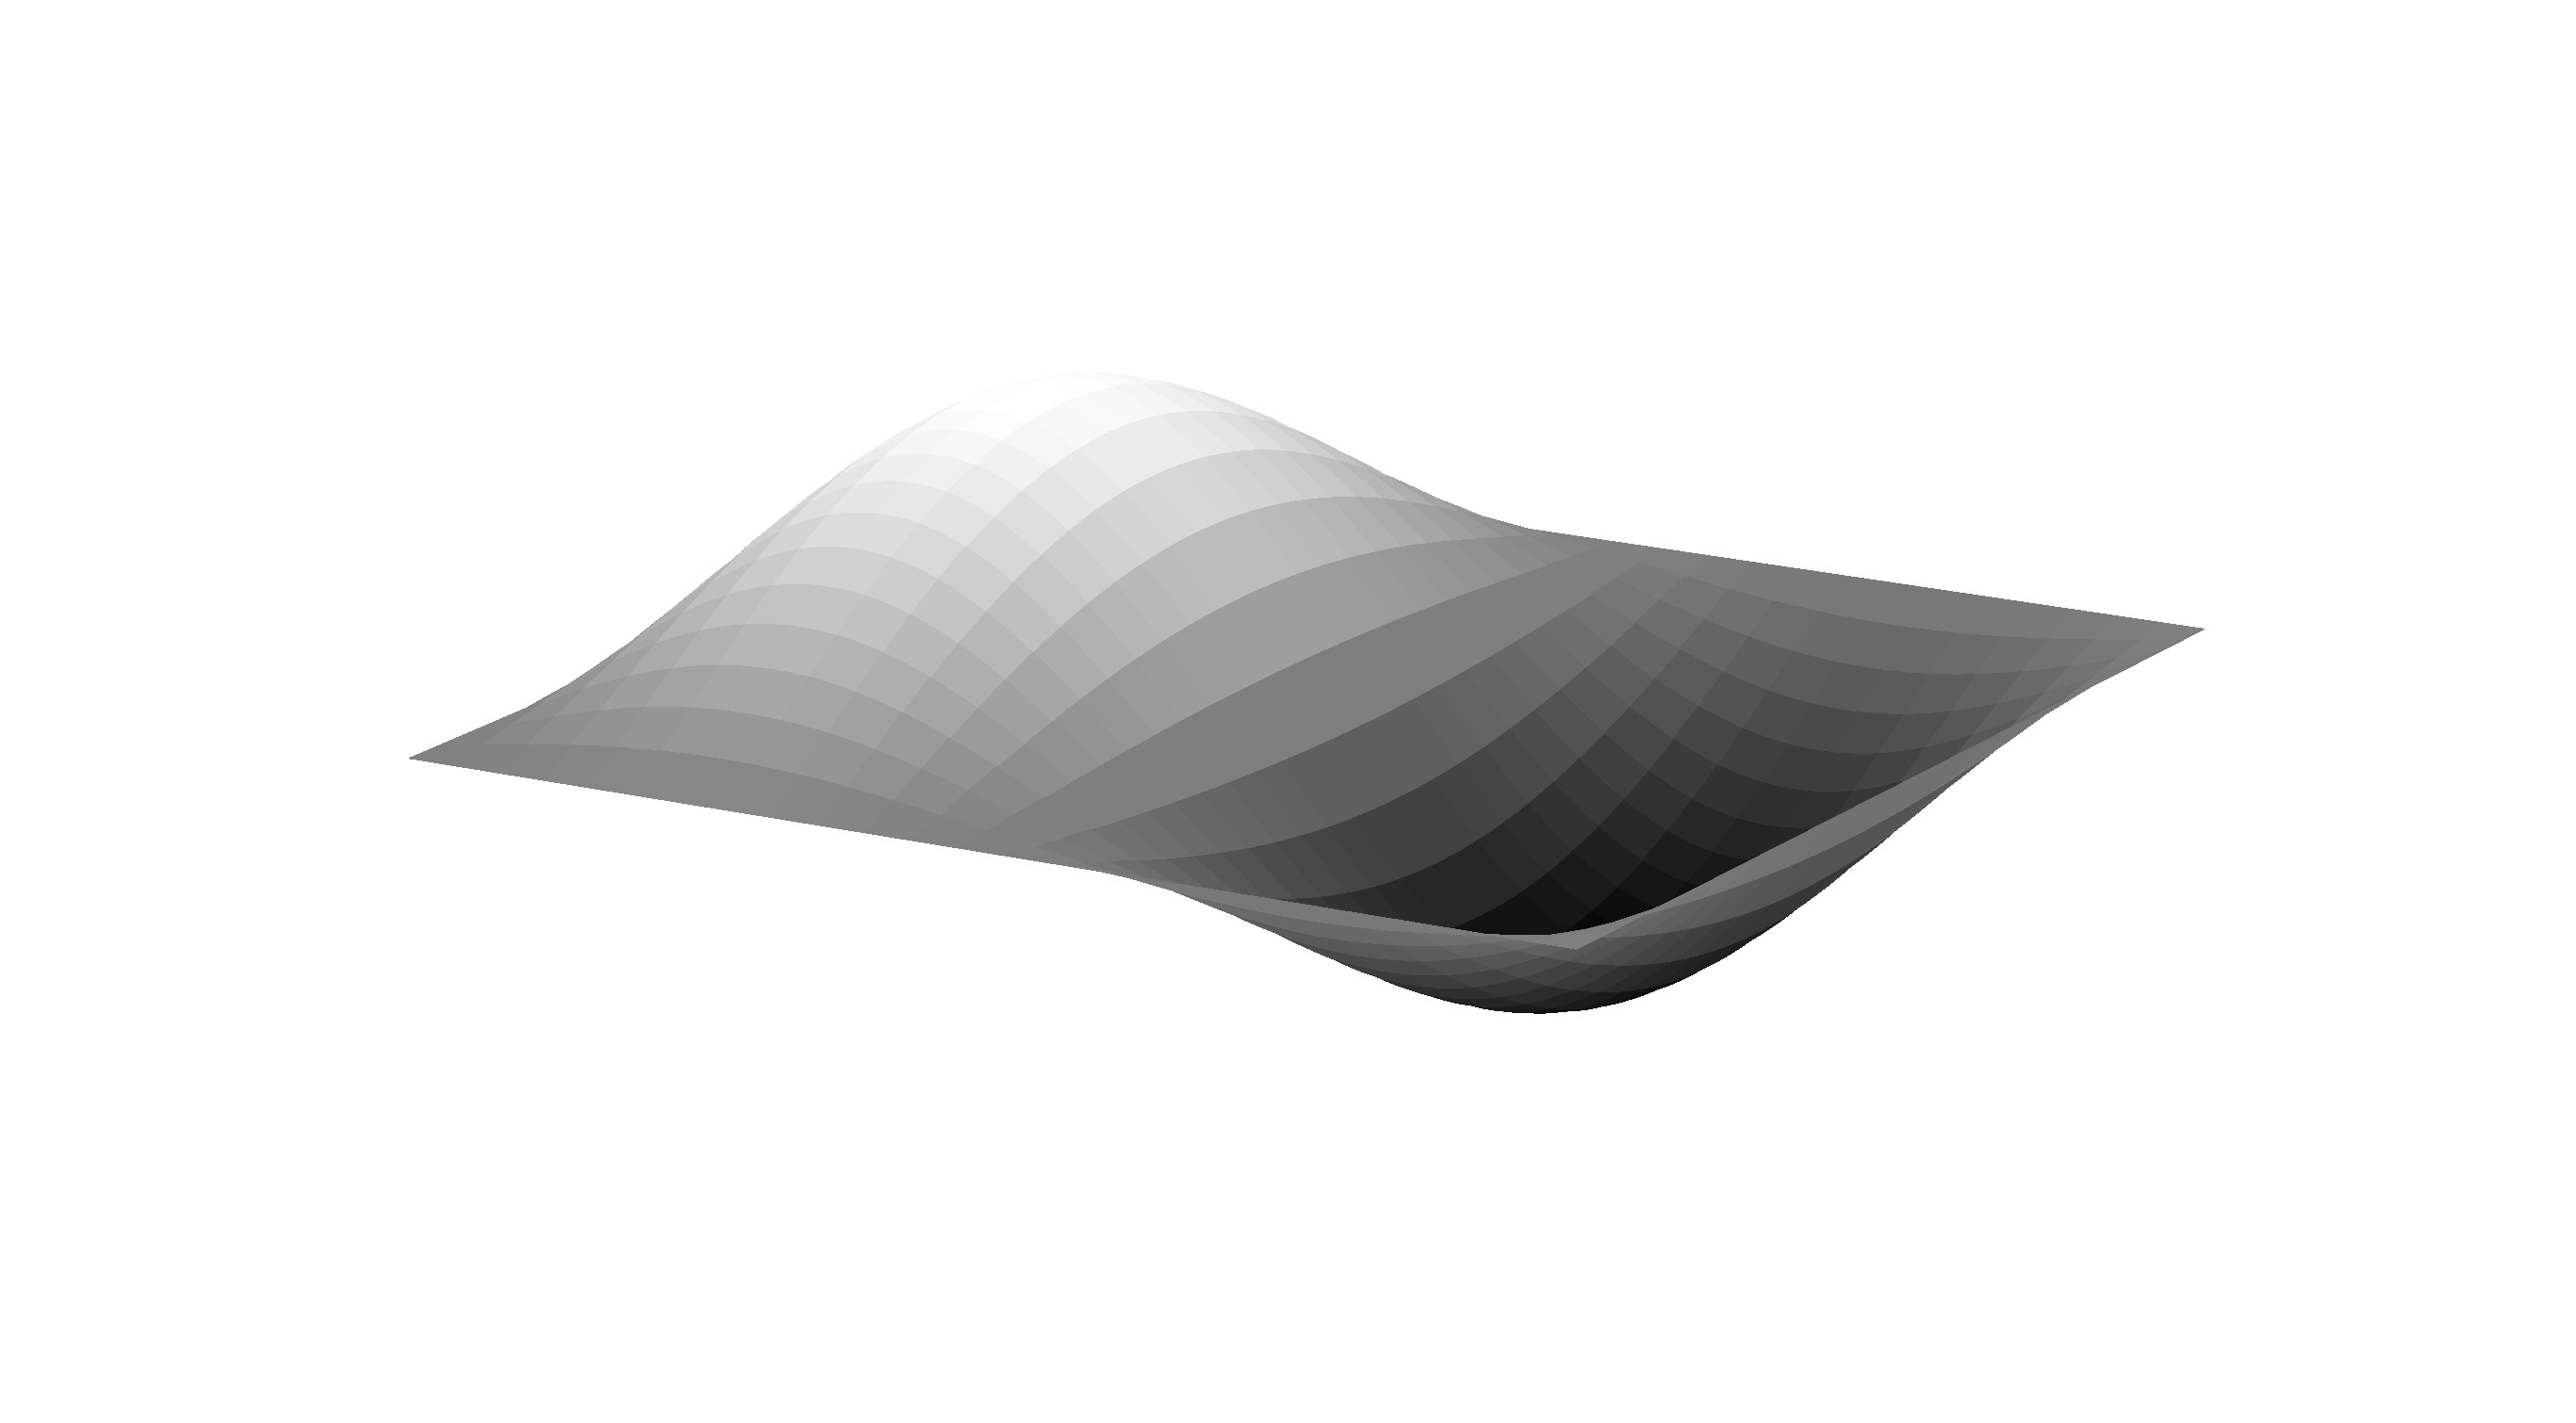
\includegraphics[width=\textwidth]{/modes/mode12.eps}
        \caption*{(1,2)}
    \end{subfigure}\\
    \begin{subfigure}[b]{0.49\textwidth}
        \centering
        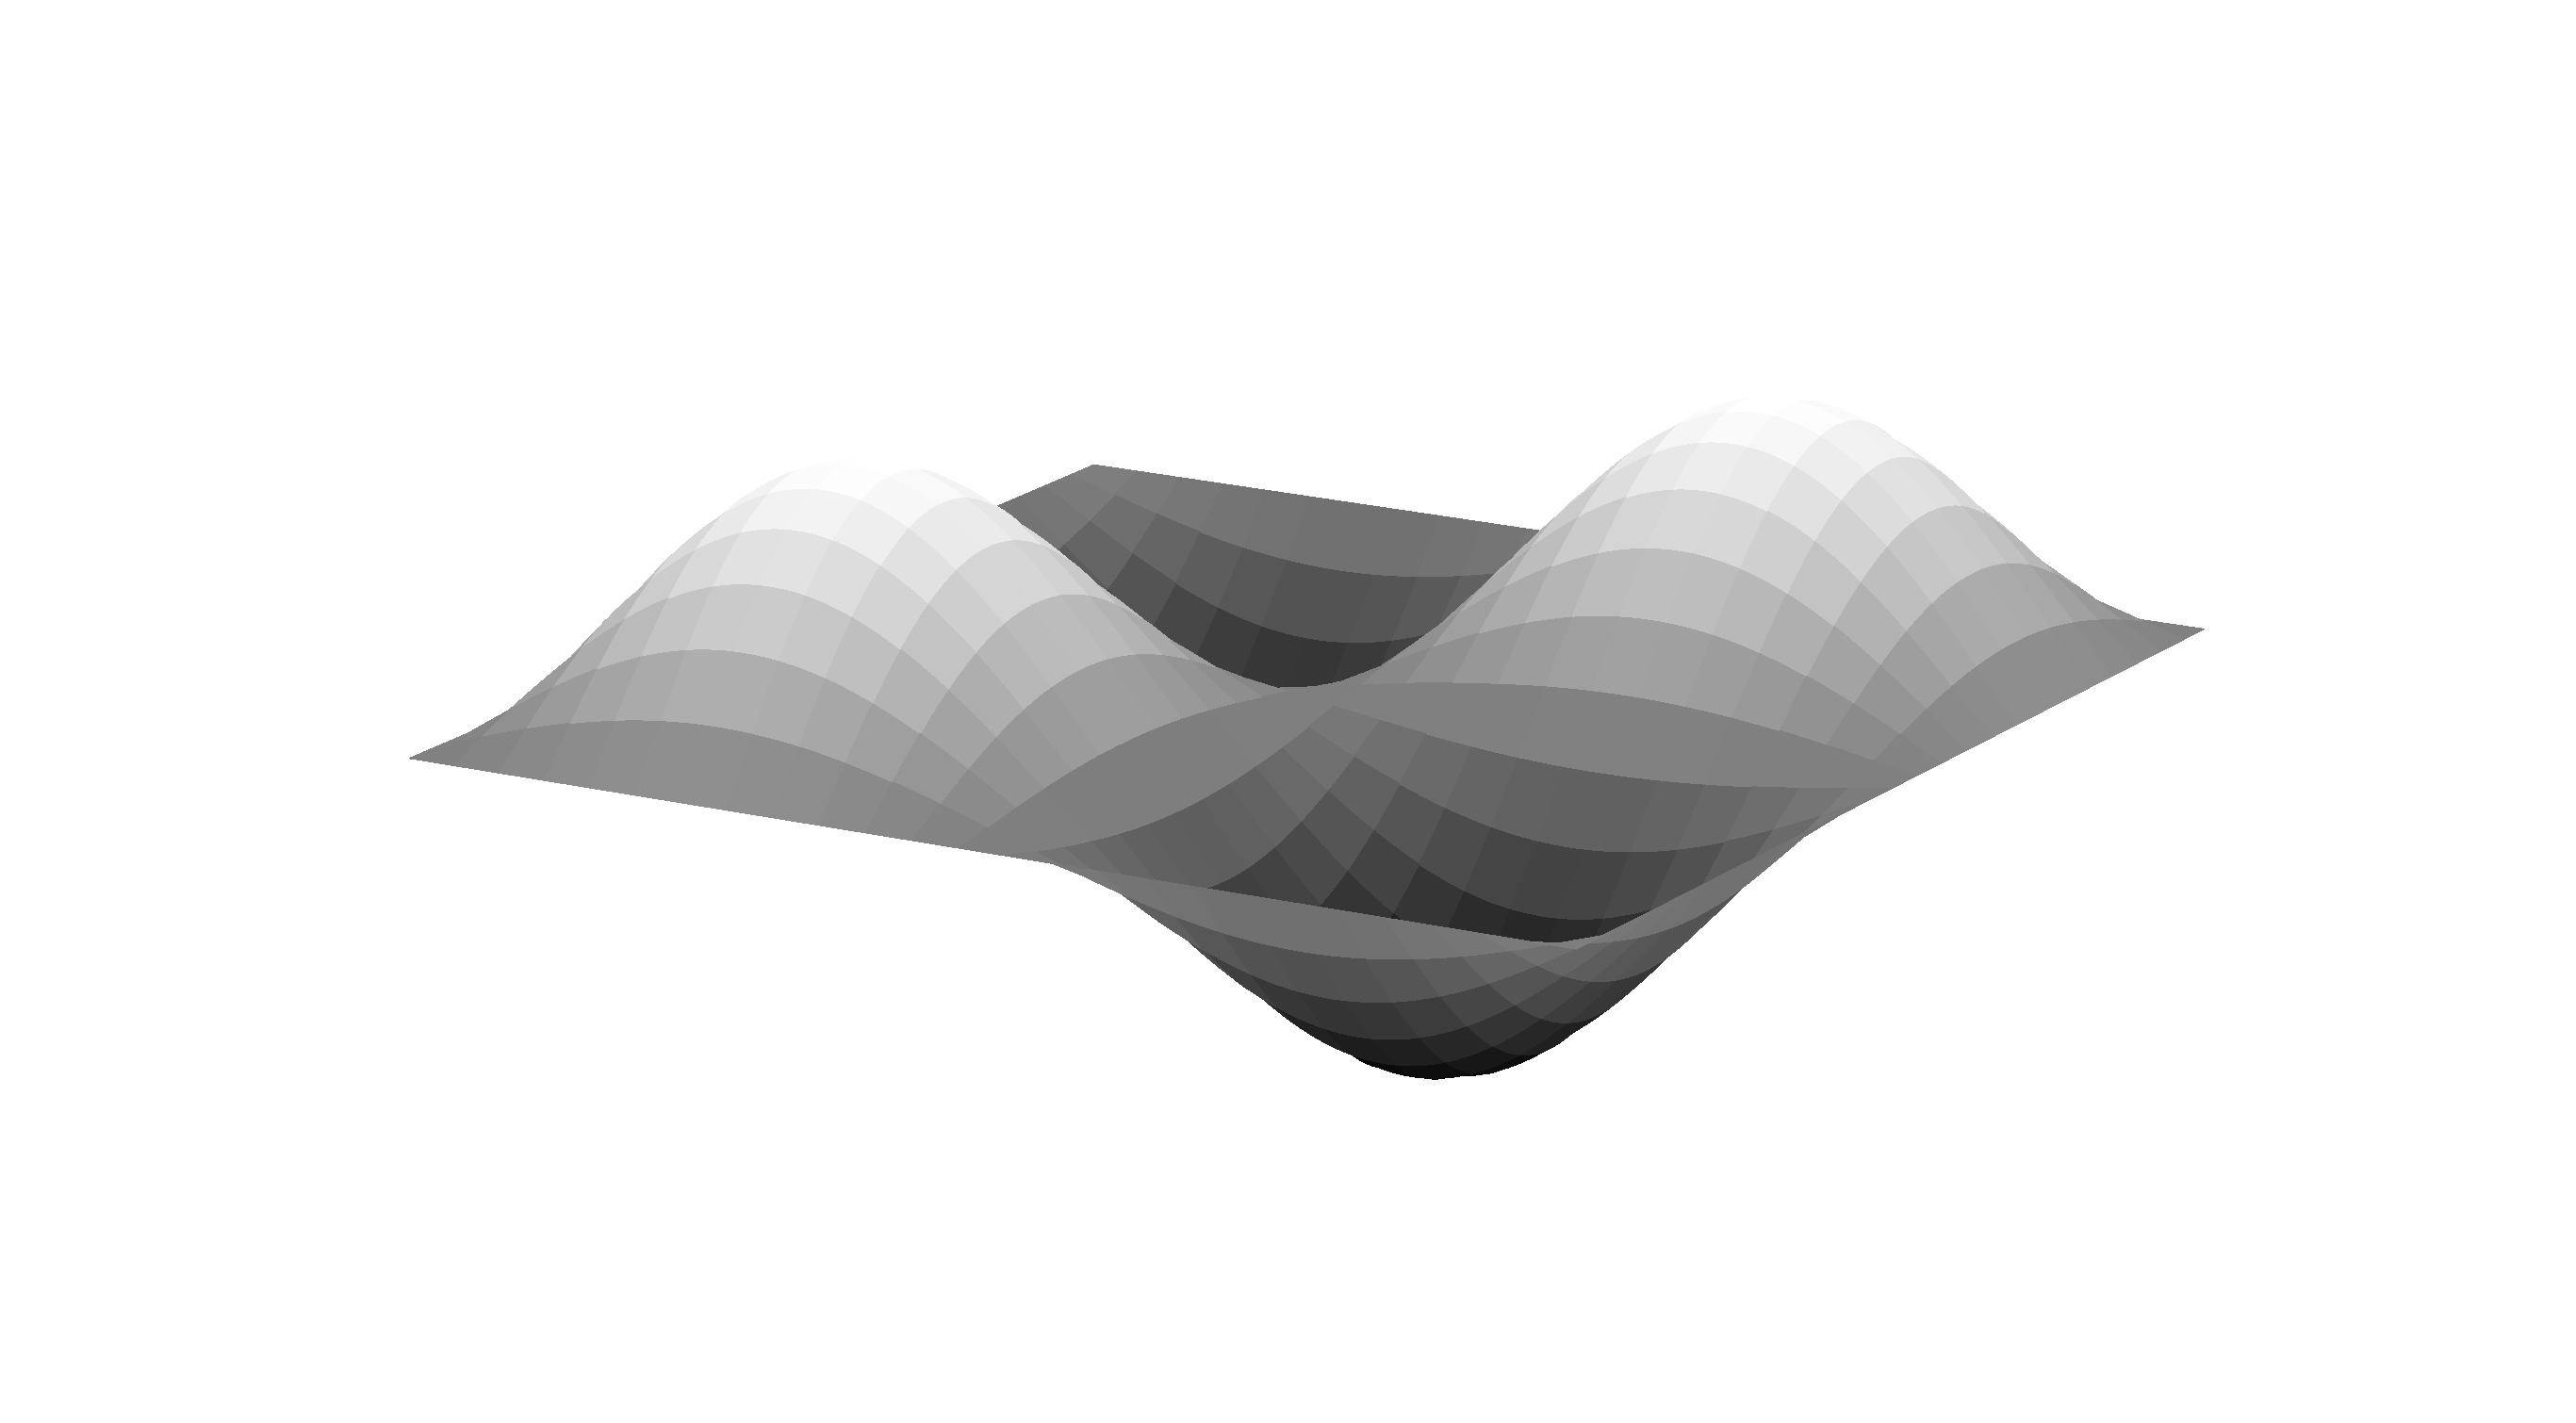
\includegraphics[width=\textwidth]{/modes/mode22.eps}
        \caption*{(2,2)}
    \end{subfigure}
    \hfil
    \begin{subfigure}[b]{0.49\textwidth}
        \centering
        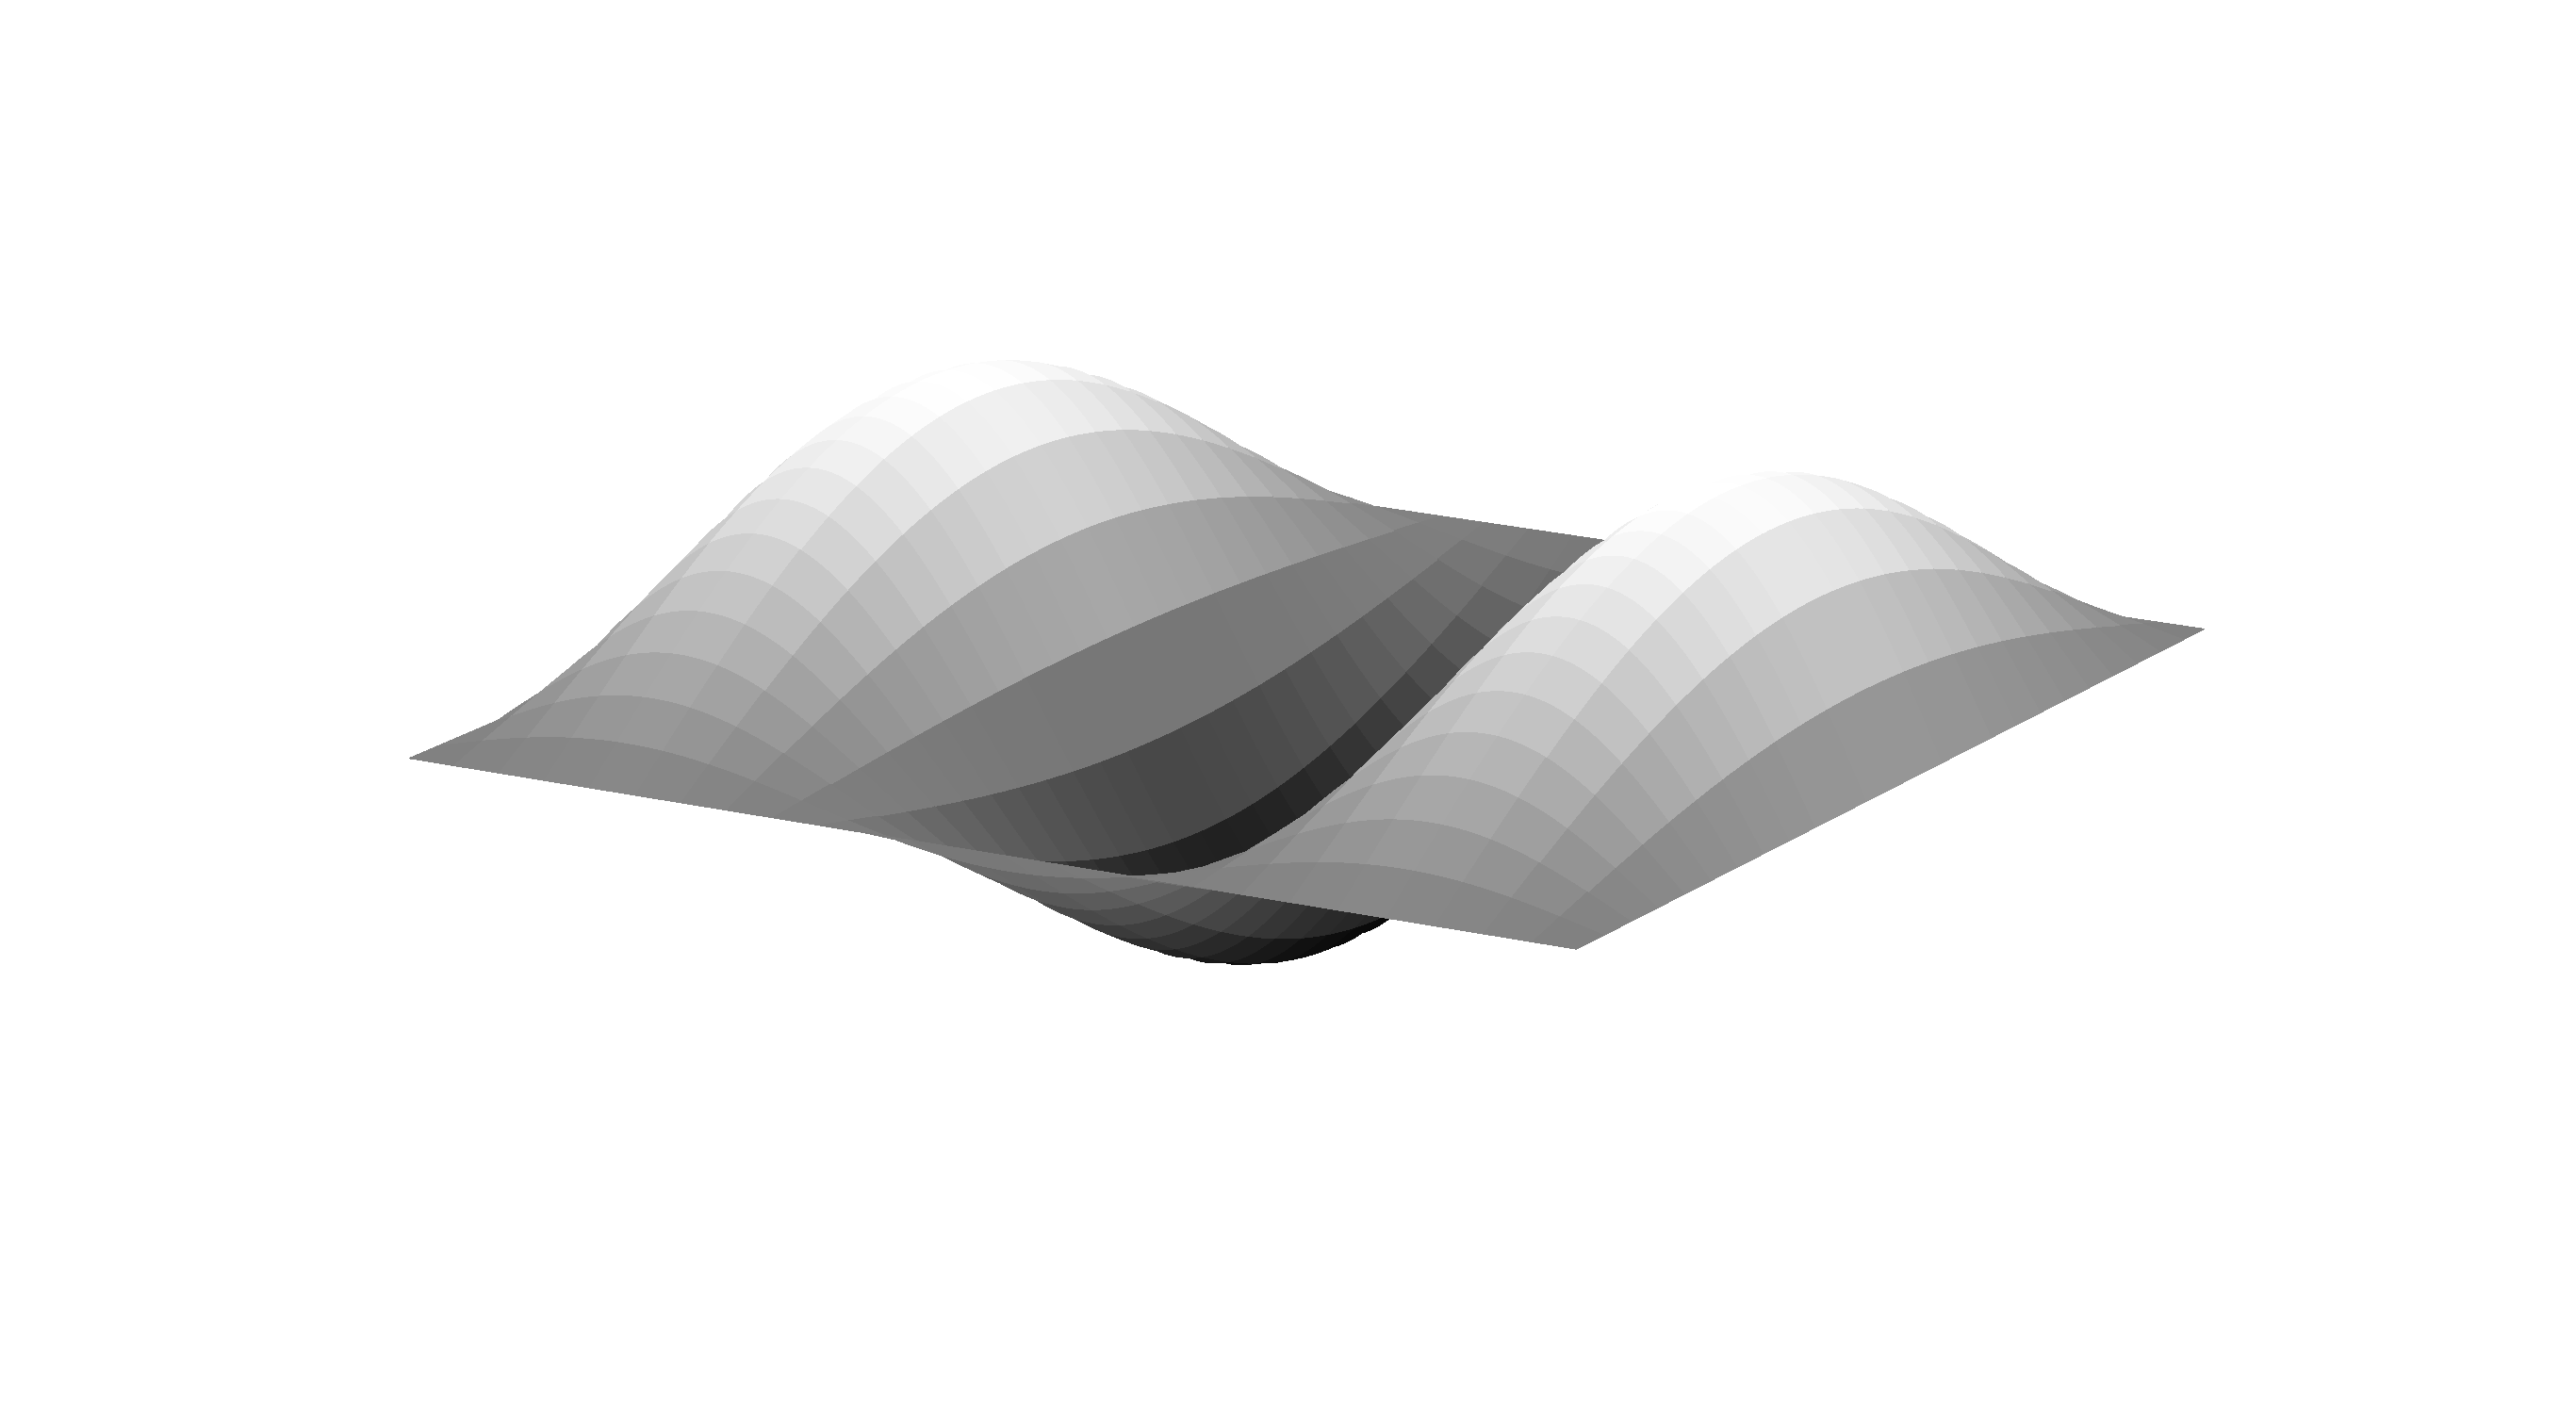
\includegraphics[width=\textwidth]{/modes/mode13.eps}
        \caption*{(1,3)}
    \end{subfigure}\\
        \begin{subfigure}[b]{0.49\textwidth}
        \centering
        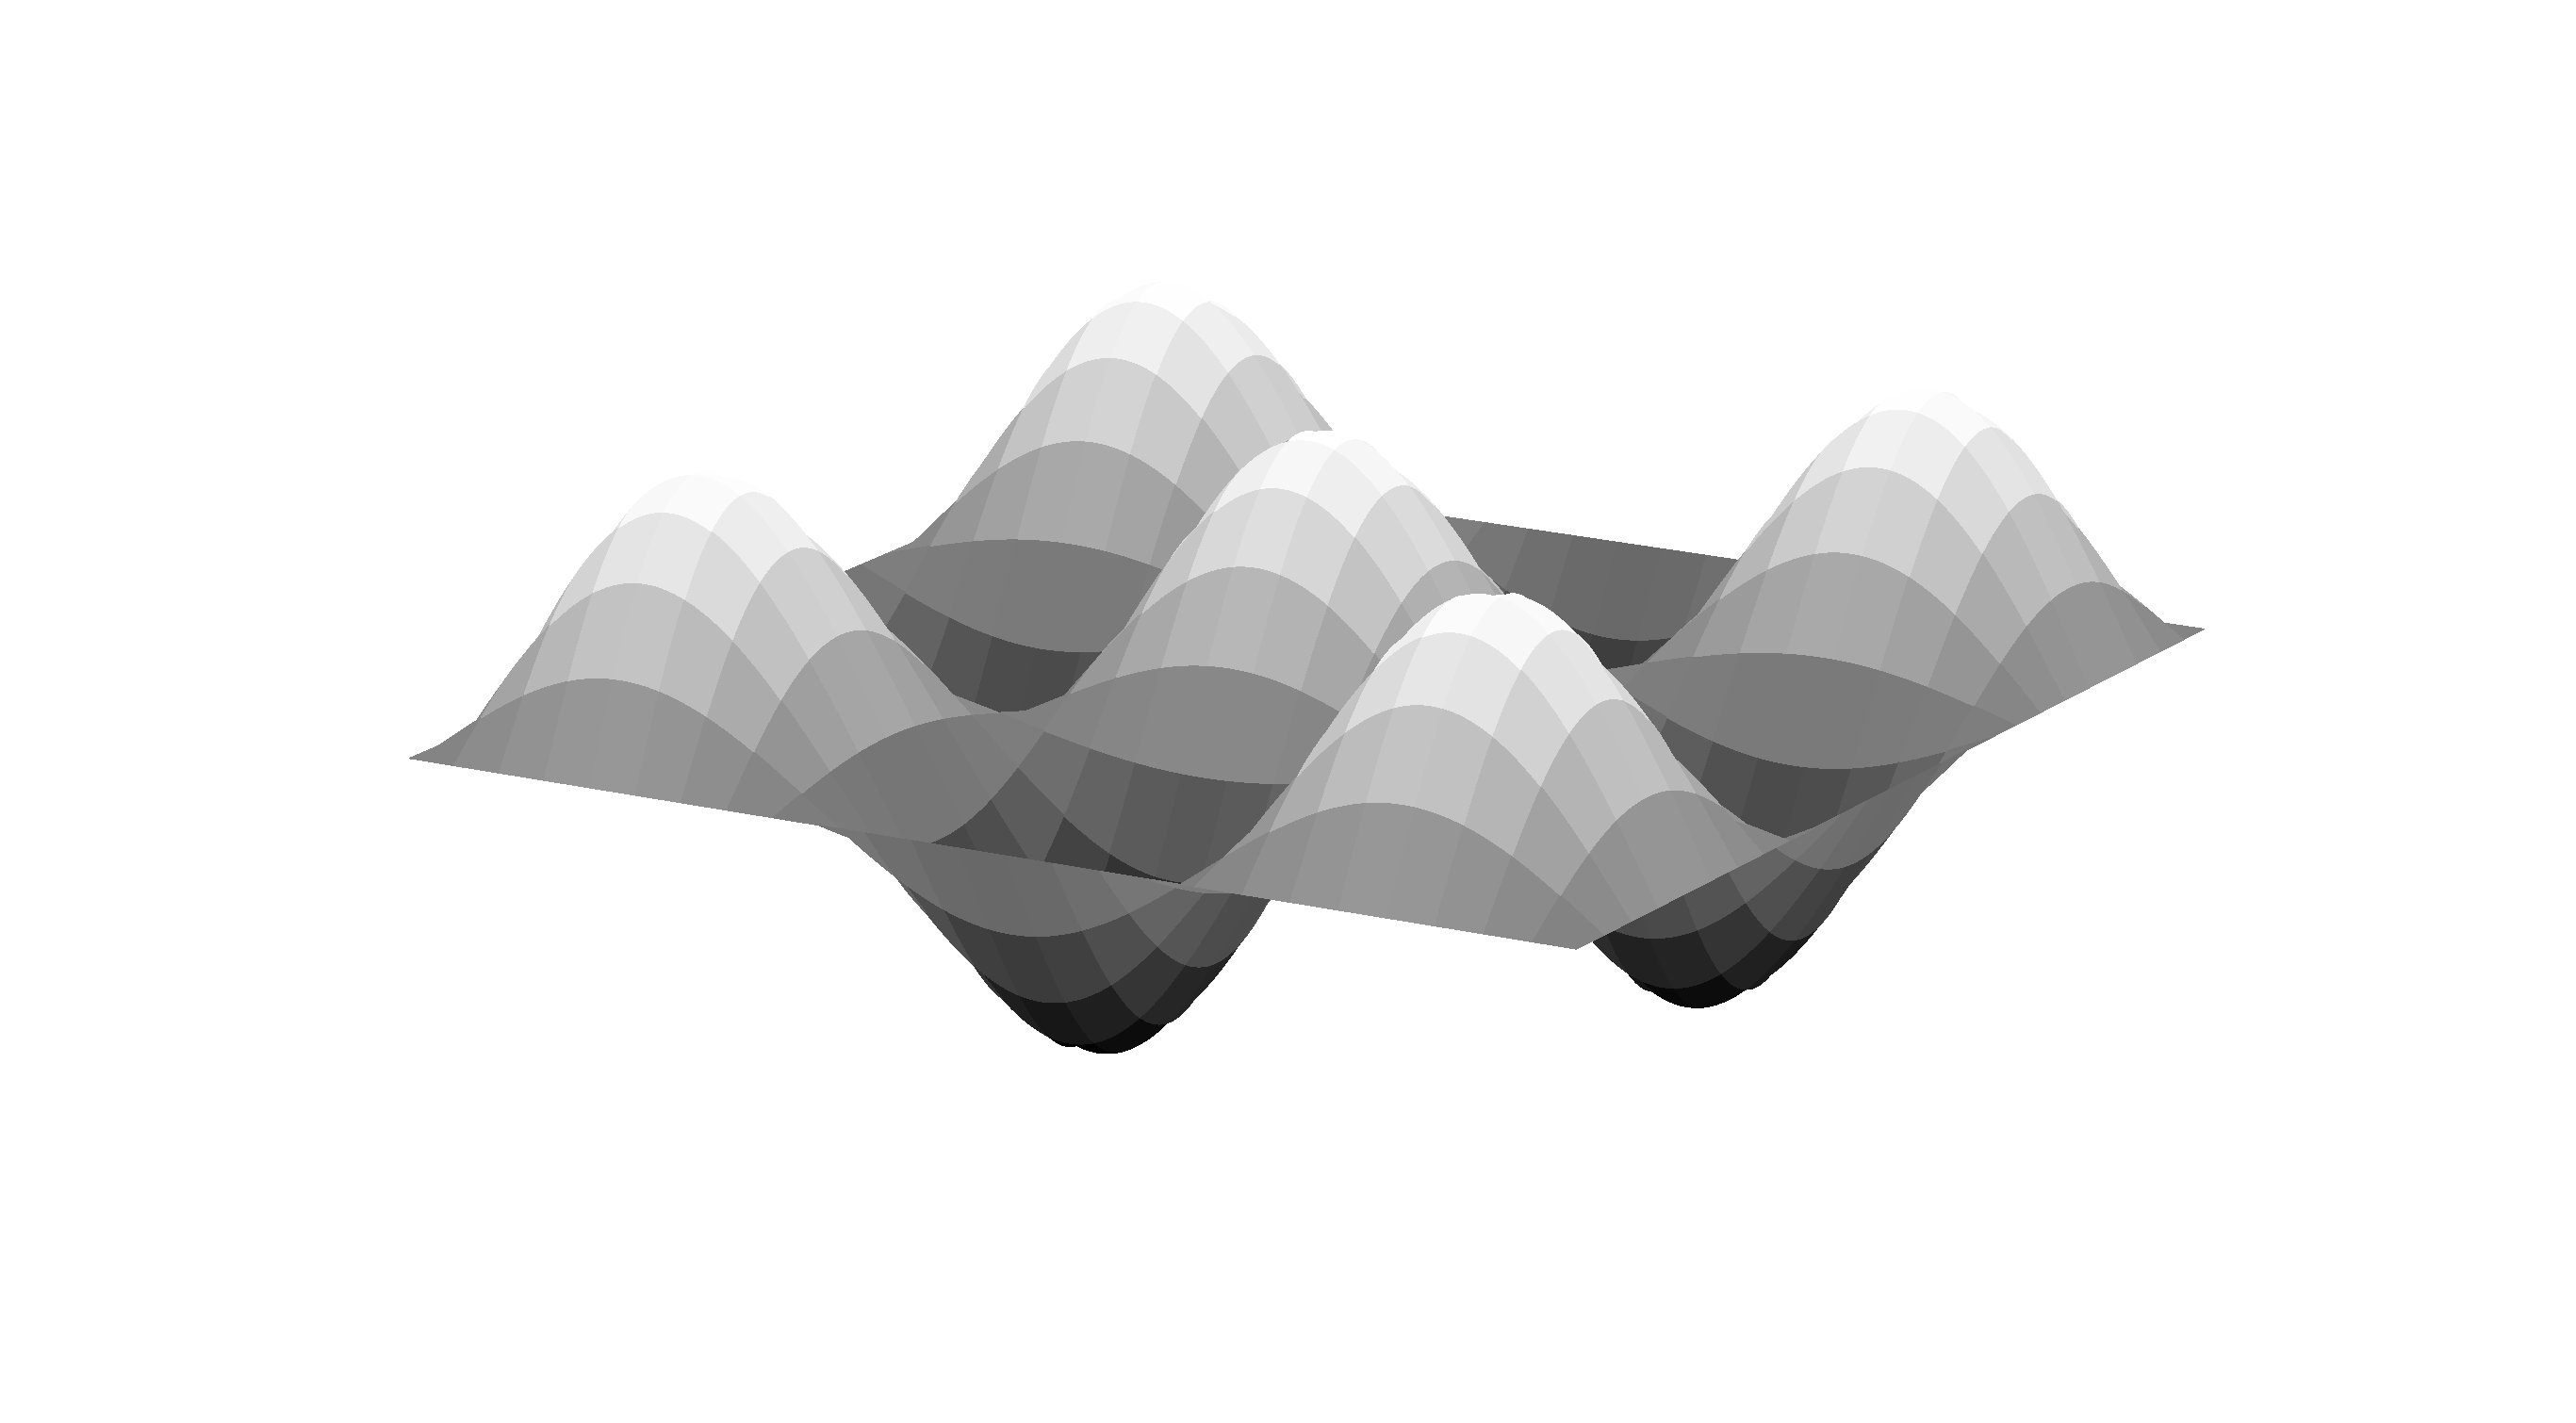
\includegraphics[width=\textwidth]{/modes/mode33.eps}
        \caption*{(3,3)}
    \end{subfigure}
    \hfil
    \begin{subfigure}[b]{0.49\textwidth}
        \centering
        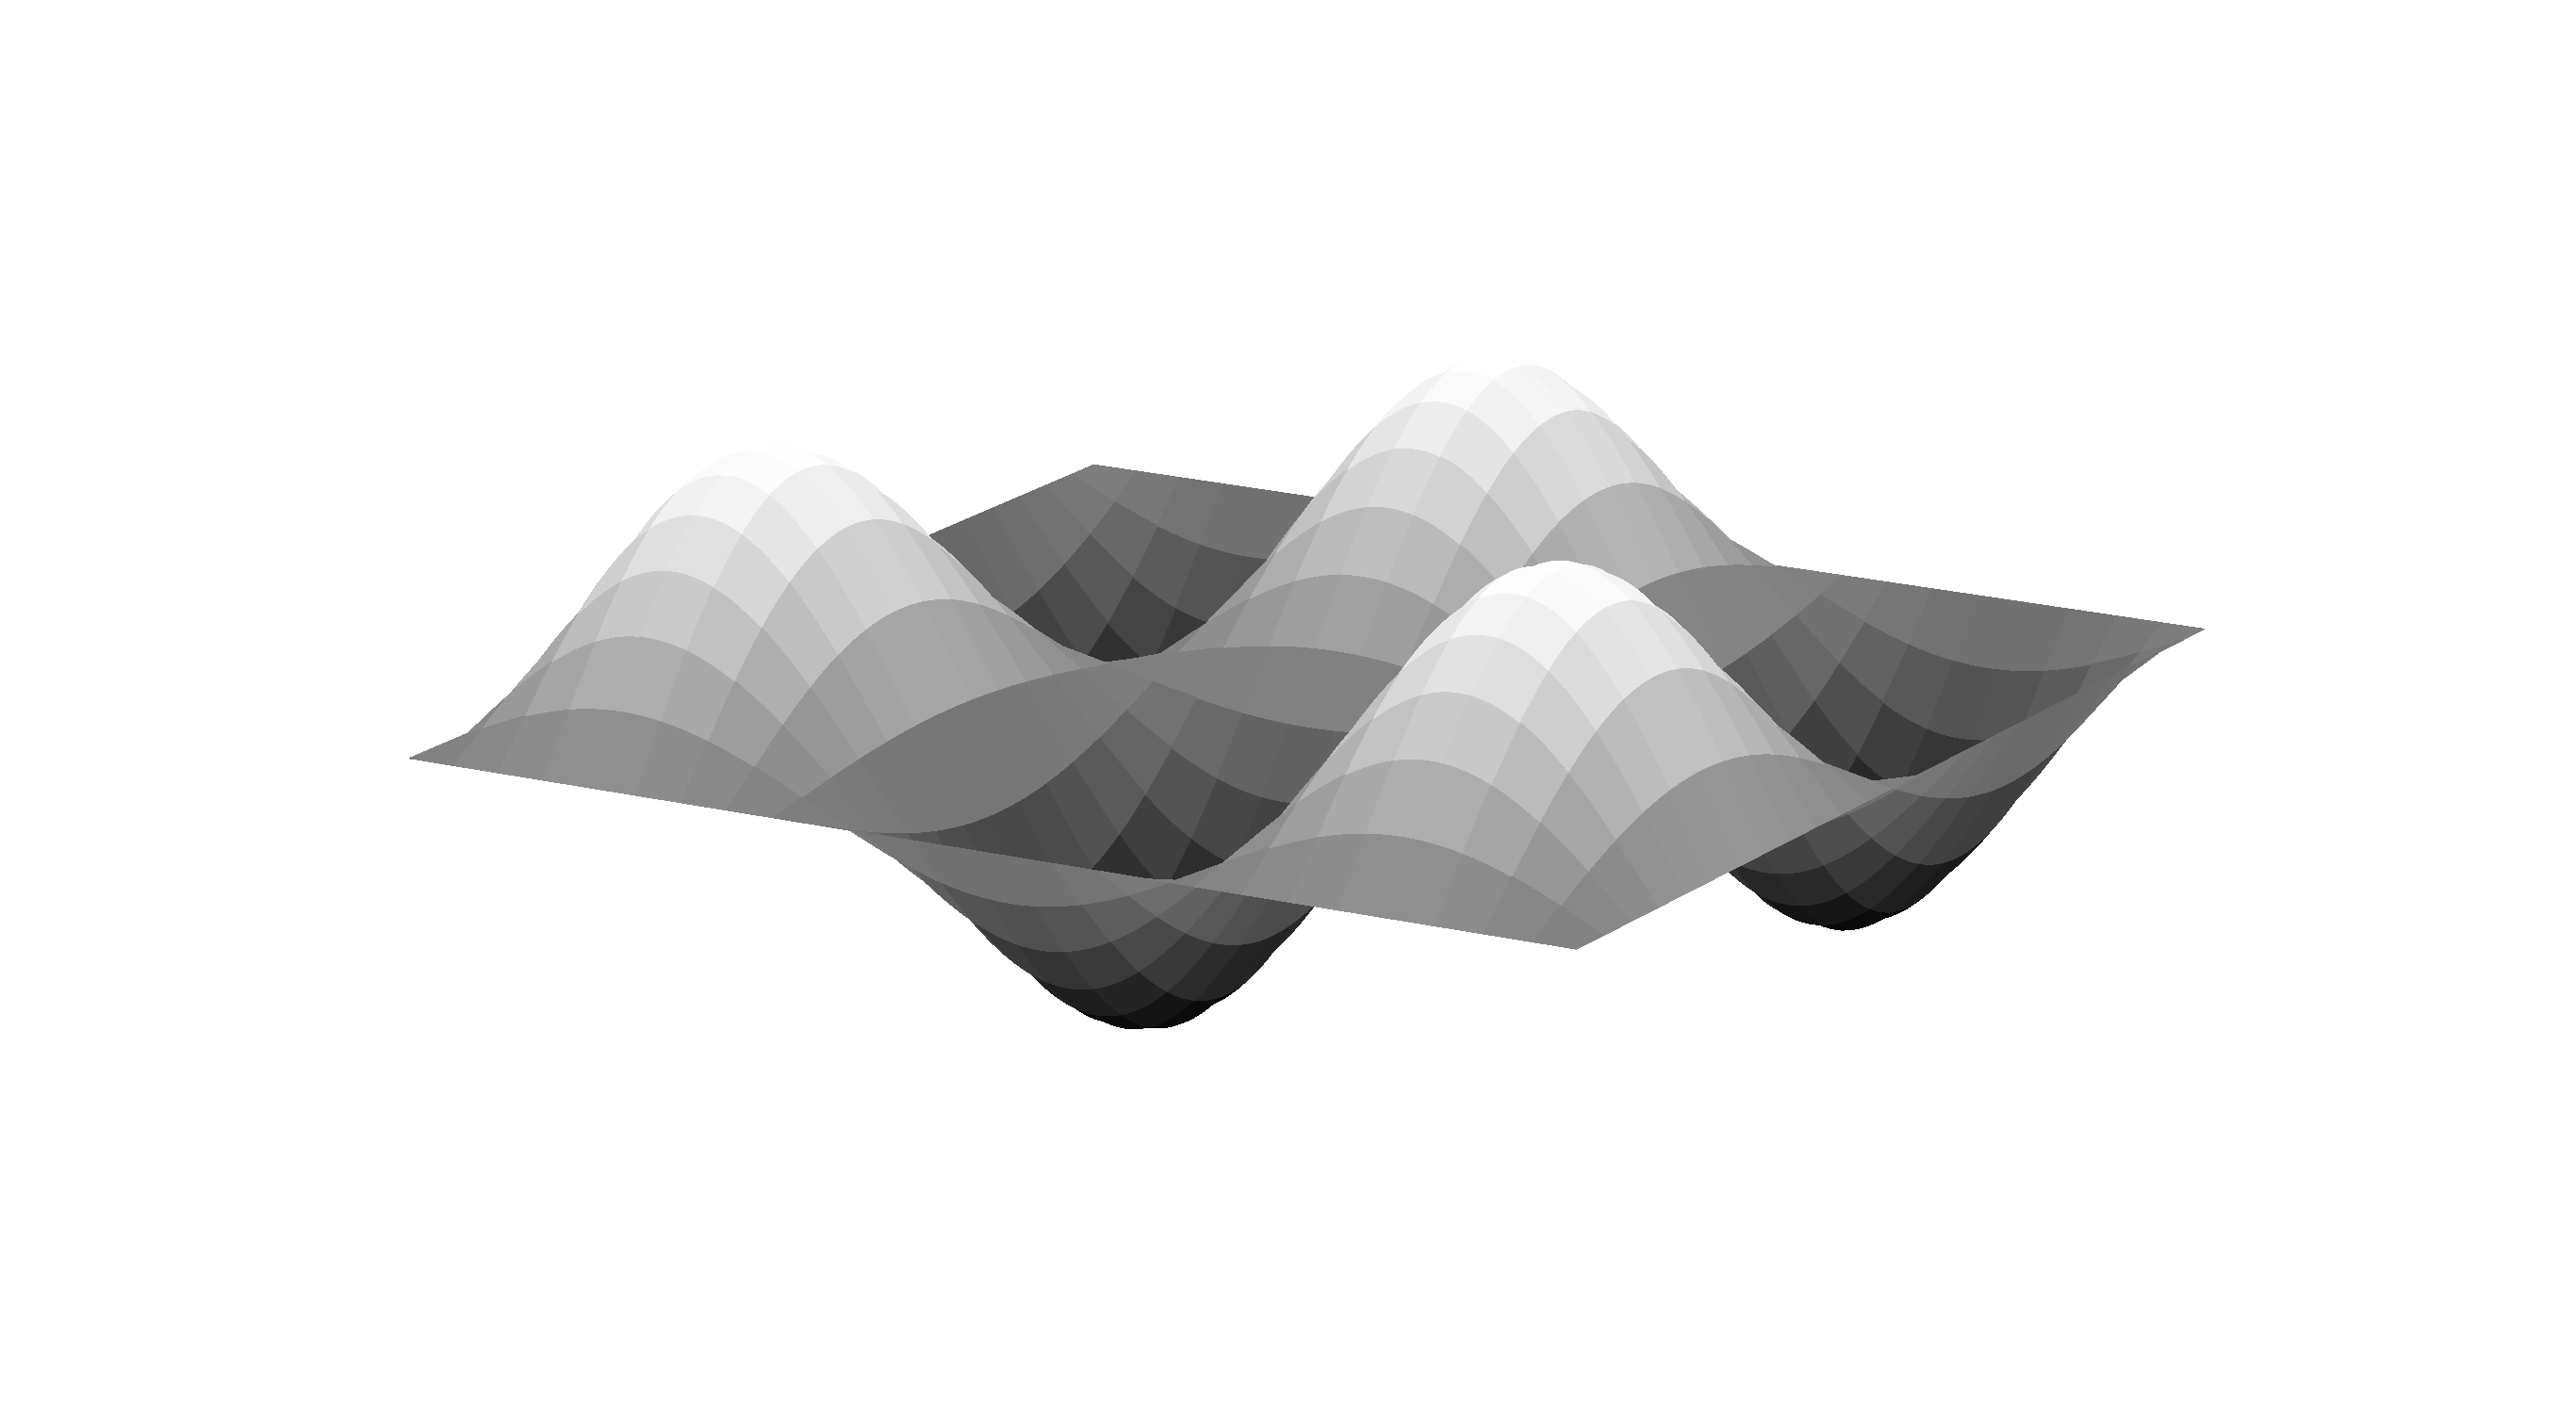
\includegraphics[width=\textwidth]{/modes/mode23.eps}
        \caption*{(2,3)}
    \end{subfigure}
\caption{Examples of vibrational mode shapes $(m, n)$ for the square membrane with all amplitudes normalized to unity.}
\label{fig:modeshape}
\end{figure}

Later we will mostly refer to a specific mechanical angular eigenfrequencies as $\Omega_m$, but the previous definition $\Omega_{m,n}$ is still valid.

\subsection{Effective mass} \label{sec:eff_mass}
In most treatments of optomechanical systems, the mechanical resonator is treated as a one-dimensional harmonic oscillators. However, the square membrane is in reality a three-dimensional object, but assumed two-dimensional as mentioned in the previous section. Introducing an effective mass is a convenient way of mapping the quasi two-dimensional harmonic oscillator onto a one-dimensional. The concept is fairly simple; not all of the membrane is moving in the same way. If we for example compare the displacement of a point on the anti-node with that of a node, they do not travel the same distance over time or at the same velocities. For a membrane this mass reduction can be found by comparing the one-dimensional mean kinetic or potential energy with the same in two-dimensions. The mean potential energy of a one-dimensional harmonic oscillator is $\langle E_{pot} \rangle = m\Omega_{m}^2\langle x(t)^2 \rangle$. For a two-dimensional membrane resonator we calculate the mean potential energy by integrating all the potential energies of all infinitesimal mass elements $\rho h dS$, weighted with $w(u,v,t)$ from equation \eqref{eq:modeshape}, where $dS = dudv$ is the infinitesimal surface element

\begin{equation}
\begin{split}
\langle E_{pot} \rangle & = \rho h \Omega_{m,n}^2 \int_S dS w(u,v,t)^2 \\
 & = \rho h \Omega_{m,n}^2 \langle T(t)^2 \rangle \int_0^l \sin^2(k_m u) du \int_0^l \sin^2(k_n v) dv.
\end{split}
\end{equation}
\noindent
Each integral yields a factor of $l/2$ due to the boundary conditions introduced previously. The potential energy for the membrane harmonic oscillator is

\begin{equation}
\langle E_{pot} \rangle = \frac{\rho h l^2 \Omega_{m,n}^2}{4} \langle T(t)^2 \rangle,
\end{equation}
\noindent
where $\rho hl^2 = m$. We define an effective mass 

\begin{equation}
m_{eff} \equiv \frac{m}{4},
\end{equation}
\noindent
which in comparison translates into a point mass one fourth of the original mass placed on an anti-node. Should the point mass move away from the anti-node it would correspond to an increase in effective mass. It is not a general result that the effective mass is independent of mode number, but a consequence of the spacial geometry of a square membrane. This is for example not true for a circular membrane (see \cite{Wilson2011}). Using the membrane properties from table \ref{tab:memprop} we get an effective mass of $m_{eff} \approx 10.5$ \SI{}{\nano\gram}.
%
%The laser spot is not just a point on the membrane but has a finite area coverage, but if the spot size is much smaller than the membrane wavelength, we do not have to worry about the overlap integral between the spot size and mechanical mode shapes.

\subsection{Fourier series and transform}
Fourier series is a useful tool for representing functions for which Taylor series expansion are not possible, an example being the Dirac delta function. It states that any time-dependent process in a linear system can be expressed as a superposition of sinusodial functions, but the process must fulfil the Dirichlet conditions \parencite{riley2006}. This means that a process $f(t)$ with a periodicity $T$ can be written as:

\begin{align}
f(t) & = \sum_{n = -\infty}^\infty c_r e^{i\omega_r t} \\
c_r & = \frac{1}{T}\int_{-T/2}^{T/2}dtf(t)e^{-i\omega_r t},
\end{align}
\noindent
with $\omega_r = 2\pi r/T$. The above treatment can be generalized to the Fourier integral transform by taking the limit $T \to \infty$ in the Fourier series expansion above. This gives the following definition of the Fourier transform $\mathcal{F}$ and its inverse $\mathcal{F}^{-1}$:

\begin{align}
\mathcal{F}[f(t)] & \equiv f(\omega) = \int_{-\infty}^{\infty}dtf(t)e^{-i\omega t} \\
\mathcal{F}^{-1}[f(\omega)] & \equiv x(t) =\frac{1}{2\pi} \int_{-\infty}^{\infty}d\omega f(\omega)e^{i\omega t},
\end{align}
\noindent
the only requirement being that $\int_{-\infty}^{\infty}dt\left|f(t)\right|$ is finite.

\subsection{Power spectral density}
Let us consider a random fluctuating function $x_n(t) \in \Re$, for example be a Johnson noise voltage generated in a resistor at a finite temperature, which is connected in parallel with a capacitor \cite{davenportroot}. Or consider the movement of our membrane caused by Brownian motion due to its finite temperature. Both of theses cases are stationary processes, meaning that $x_n(t)$ and $x_n(t + \tau)$, separated by a small time-shift $\tau$, have the same statistical properties. An important statistical measure is the autocorrelation:

\begin{equation}
\langle x_n(t)x_n(t + \tau)\rangle = \lim_{T \to \infty}\int_{-T/2}^{T/2}dt~x_n(t)x_n(t + \tau).
\end{equation}
\noindent
The Fourier transform of the autocorrelation of $x_n(t)$ is called the double-sided power spectral density

\begin{equation}
S_{xx}(\omega) = \int_{-\infty}^{\infty}d\tau\langle x_n(t)x_n(t + \tau)\rangle e^{-i\omega \tau} = \left|\mathcal{F}[x(t)]\right|^2,
\label{eq:PSD}
\end{equation}
\noindent
which is a consequence of the Wiener-Khinchin theorem \cite{riley2006}, stating that the autocorrelation of a stationary random process has a spectral decomposition given by the power spectrum of that same process. The variance of x(t) can be shown to be
\begin{equation}
\langle x_n(t)^2 \rangle = \frac{1}{2\pi}\int_{-\infty}^{\infty}d\omega~S_{xx}(\omega).
\label{eq:inverse_ft}
\end{equation}
\noindent
Since $x_n(t)$ is assumed real, it can be shown that $S_{xx}(\omega) = S_{xx}(-\omega)$. This property is used in defining the single-sided power spectral density

\begin{equation}
S_x(\omega) \equiv 2S_{xx}(\omega).
\end{equation}

\subsection{One-dimensional damped harmonic oscillator} \label{sec:1D_ho}
\subsubsection{Time domain analysis}
We showed in section \ref{sec:eff_mass} that we can map the two-dimensional membrane onto a one-dimensional model, by introducing an effective mass. In this chapter we will present some of the general results of the one-dimensional damped harmonic oscillator, which is equivalent to the textbook example of mass a suspended on a spring system. At least for us doing cavity optomechanics. In fact a mirror on a spring is the canonical example of a cavity optomechanical system.

We already considere the solution of the rather dull case of a harmonic oscillator with no damping in chapter \ref{sec:vib_modes}, so we will skip it and jump directly to introducing a viscous damping term $\Gamma_m = b/m$, which is proportional to the velocity $\dot{x}(t)$ (the dot symbolises a time derivative). We can write out the equations of motion of the system

\begin{align}
m\ddot{x}(t) + b\dot{x}(t) + kx(t) &= 0 \\
\ddot{x}(t) + \gamma\dot{x}(t) + \omega_{m,n}^2x(t) &= 0,
\end{align}
\noindent
whit $\Omega_{m} = \sqrt{k/m}$, where $k$ is the spring constant and $m$ the mass. We can easily solve this exactly and show that it is an exponentially decaying cosine, if the damping term is relatively small ($\Omega_{m} \gg \Gamma_m$) \cite{young2003} (see figure \ref{fig:damped_osc})

\begin{equation}
x(t) = x_0e^{-\frac{\gamma}{2}t}\cos(\Omega_0t + \varphi),
\end{equation}
\noindent
where $\Omega_0 = \sqrt{\Omega_{m}^2 - \left(\frac{\Gamma_m}{2}\right)^2}$, $x_0$ is the amplitude and $\varphi$ is the phase. There are three different damping regimes:

\begin{itemize}
\item Underdamped ($\Omega_m > \frac{\Gamma_m}{2}$): The system oscillates with a slightly different frequency, compared to the undamped case, and slowly decays to its resting position (equilibrium).
\item Critically damped ($\Omega_m = \frac{\Gamma_m}{2}$): The system returns to equilibrium as quickly as possible without oscillating.
\item Overdamped ($\Omega_m < \frac{\Gamma_m}{2}$): Returns exponentially to equilibrium without oscillating, but slower for large $\Gamma_m$ and can overshoot the equilibrium position as seen in figure \ref{fig:damped_osc}.
\end{itemize}

\begin{figure}[H]
\centering
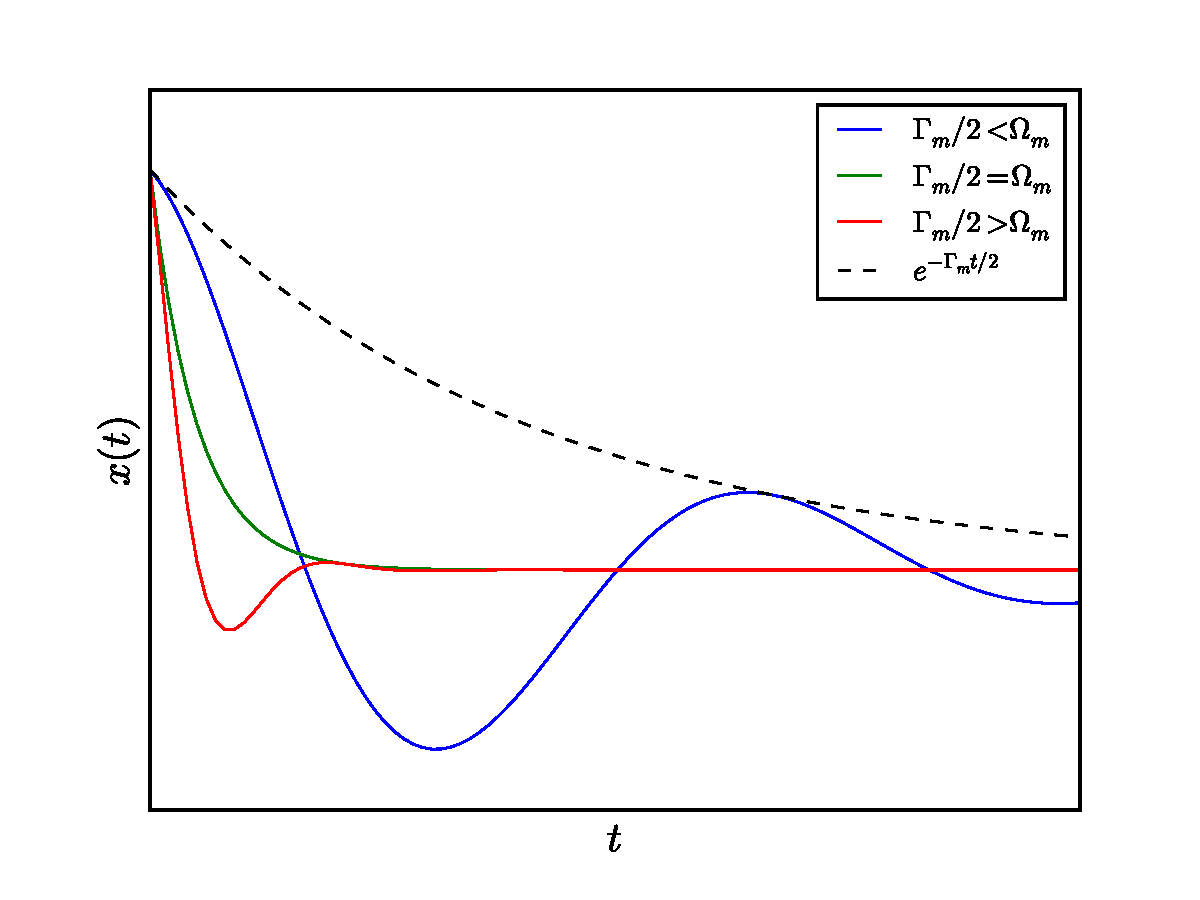
\includegraphics[scale=0.6]{damped_oscillator.pdf}
\caption{Behaviour of a damped harmonic oscillator for three different damping coefficients regimes.}
\label{fig:damped_osc}
\end{figure}

The result is a basic result that all physicists should know, but none the less, it is an important result in optomechanics. The $1/e$-time is what defines the ringdown time $\tau = 1/\Gamma_m$, i.e. how quickly energy dissipates from the system when excited. This is used for both cavities and membranes to characterize their dissipation rates. Another example for why this is important, is that membranes could potentially be used as memory, because of their slow decoherence rate.

\subsubsection{Frequency domain analysis}
Another way of solving the equation of motion of a one-dimensional oscillator is by using the Fourier transform. This time we will add an external force $F_{ext}(t)$ to the model and write out the equations of motion. Performing the Fourier transform is a trivial matter since we are dealing with a differential equation ($\frac{d}{dt} \rightarrow -i\Omega$ and $\frac{d^2}{dt^2} \rightarrow -\Omega^2$)

\begin{align}
\left(\ddot{x}(t) + \Gamma_m\dot{x}(t) + \Omega_{m}^2x(t)\right)m & = F_{ext}(t) \\
m\left[-\Omega^2 + \Omega_{m}^2 -i\Omega\Gamma_m\right]x(\Omega) & = \chi(\Omega)^{-1}x(\Omega) = F_{ext}(\Omega),
\end{align}
\noindent
where $\chi(\Omega)$ is the mechanical susceptibility of the system. We will specify the properties of the newly introduced driving force later on. We can easily write the power spectral density of the system using equation \eqref{eq:PSD}, if we assume operation near resonance $\Omega \approx \Omega_{m}$, which means that $\Omega + \Omega_{m} \approx 2\Omega$ and $\Omega/\Omega_{m} \approx 1$, while the detuning (small differences) $\Delta = \Omega_{m} - \Omega$ will still be of interest and not approximated with zero. The power spectral density takes the following form

\begin{equation}
\begin{split}
S_{xx}(\Omega) & = \left|S_{xx}^{ext}(\Omega)\chi(\omega)\right|^2 = \frac{\left|S_{xx}^{ext}(\Omega)\right|^2}{m}\left[(\Omega_{m}^2 - \Omega^2)^2 + (\Omega\Gamma_m)^2\right]^{-1} \\
& \approx \frac{\left|S_{xx}^{ext}(\Omega)\right|^2}{4m^2\Omega_{m}^2}\left[\Delta^2 + (\Gamma_m/2)^2\right]^{-1}.
\end{split}
\end{equation}
\noindent
The first line is the full mechanical power spectral density, whereas in the second line we have performed the Lorentzian approximation, see the difference in figure \ref{fig:lor_approx}. The mechanical damping coefficient $\Gamma_m$ is the full-width-half-maximum (FWHM) of the line shape.

\begin{figure}[H]
\centering
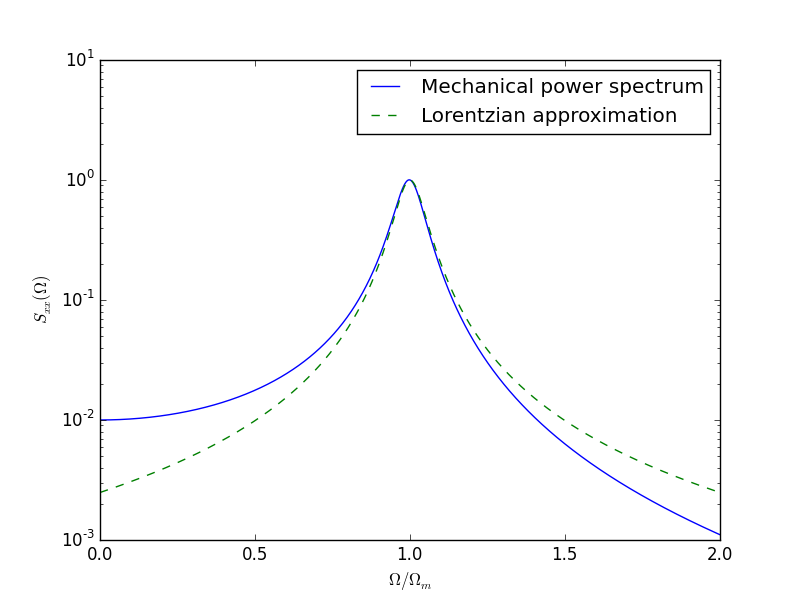
\includegraphics[scale=0.8]{lorentzian_approx.png}
\caption{Normalized power spectral density for arbitrary parameters of a mechanical oscillator (blue). The dashed (green) line is the Lorentzian approximation for the same parameters.}
\label{fig:lor_approx}
\end{figure}

\subsection{Thermal driving force}
The vibrational energy of the system is non-zero, since the membrane is energetically coupled through the mechanical damping rate $\Gamma_m$ to an environment with a finite bath temperature $T_{bath} > 0$. This coupling introduces random fluctuations due to dissipation mechanisms, causing the Brownian motion of the membrane as described by the fluctuation-dissipation theorem \cite{saulson1990}. In statistical physics the Langevin equation is used to describe the Brownian motion of a point particle, so let us introduce a Langevin force $F_{th}(t)$, which is a delta correlated stationary Gaussian process with zero-mean $\langle F_{th}(t) \rangle = 0$, meaning that forces at different times are uncorrelated. The Langevin force is described by the autocorrelation function

\begin{equation}
\langle F_{th}(t) F_{th}(t + t') \rangle = 4k_BT_{bath}m_{eff}\Gamma_m\delta(t'),
\label{eq:thermal_drive}
\end{equation}
\noindent
where $\delta(t')$ is the Dirac delta function. From this it is trivial to obtain the power spectral density using equation \eqref{eq:PSD}

\begin{equation}
S_{FF}^{th}(\Omega) = \mathcal{F}[\langle F_{th}(t) F_{th}(t + t') \rangle] = 4k_BT_{bath}m_{eff}\Gamma_m.
\end{equation}
\noindent
We can now replace the previously vaguely described term $\left|F_{ext}(\omega)\right|^2$ with $S_{FF}^{th}$ and obtain the following expression for the mechanical power spetral density:

\begin{equation}
S_{xx}(\Omega) = \left|\chi(\Omega)\right|^2S_{FF}^{th} = \frac{k_BT_{bath}\Gamma_m}{m_{eff}\Omega_{m}^2}\left[ \Delta^2 + (\Gamma_m/2)^2 \right]^{-1}.
\label{eq:full_psd}
\end{equation}

\subsection{Root mean square displacement} \label{sec:xrms}
An important question arises after introducing a thermal driving force; namely how large (or rather {\it{small}}) is the actual displacement of the vibrating membrane at room and cryogenic temperatures? The membrane fluctuates around zero displacement (equlibrium position) with variance $\langle x^2 \rangle$ due to the random nature of Langevin force $F_{th}$. We will calculate the root mean square displacement $x_{RMS} = \sqrt{\langle x^2 \rangle}$ and from the mechanical power spectral density using Parseval's theorem

\begin{equation}
\begin{split}
\langle x^2 \rangle & = \frac{1}{2\pi}\int_{-\infty}^{\infty}d\Omega S_{xx}(\Omega) \\
 & = \frac{1}{\pi}\frac{k_BT\Gamma_m}{\Omega_{m}^2m_{eff}}\int_{0}^{\infty}d\Omega\left[ \Delta^2 + (\Gamma_m/2)^2 \right]^{-1} \\
 & = \frac{k_BT}{\Omega_{m}^2m_{eff}} \label{eq:t_eff}.
\end{split}
\end{equation}
\noindent
Where we have inserted equation \eqref{eq:full_psd} in the integral and changed the interval of the integration from $-\infty \to 0$ and applied a factor of 2 to compensate. The integral can be solved using \cite{spiegel1999}

\begin{equation}
\int_{0}^{\infty}dx\left[x^2 + a^2 \right]^{-1} = \frac{\pi}{2a}.
\end{equation}
\noindent
Fortunately we end up confirming that this kind of thermal noise gives the equipartition theorem $m_{eff}\Omega_{m}^2\langle x^2 \rangle = k_BT$, which states that the average potential energy is equal to $k_BT/2$ at thermal equilibrium . This is a nice sanity check to see if we made any mistakes so far. Finally, we can write the expression for the root mean square displacement by taking the square root

\begin{equation}
x_{RMS} = \sqrt{\frac{k_BT}{\Omega_{m}^2m_{eff}}}.
\label{eq:rms}
\end{equation}
\noindent
We can find the effective temperature of the membrane from its spectrum, by taking the area underneath the mechanical resonance peak as shown in figure \ref{fig:mem_temp}.

\begin{figure}[H]
\centering
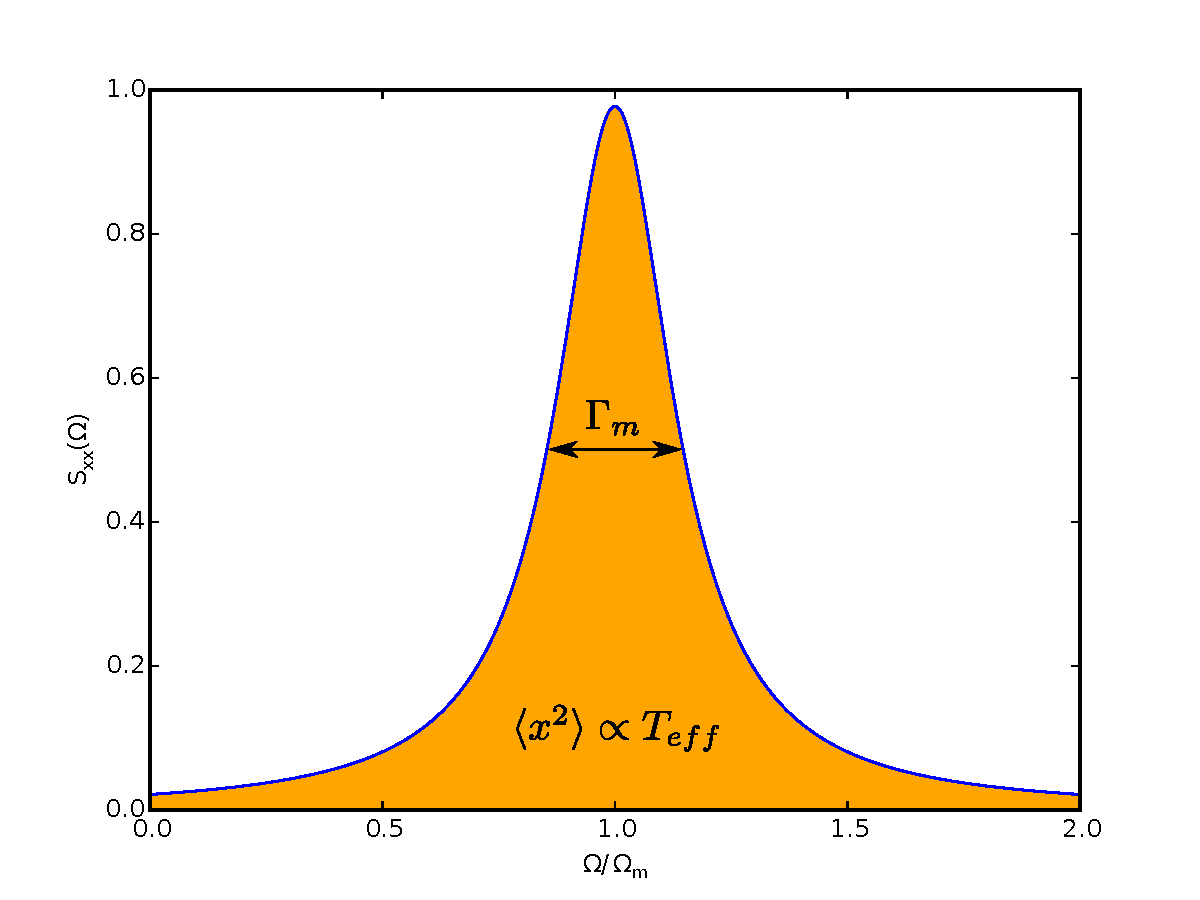
\includegraphics[scale=0.6]{rms.pdf}
\caption{Normalized Lorentzian line shape, representing the mechanical resonance, where $\Gamma_m$ is the width and the area is proportional to the membrane effective temperature $T_{eff}$.}
\label{fig:mem_temp}
\end{figure}

Let us end this chapter by calculating the root mean square displacement for the fundamental mechanical mode at typical working temperatures, i.e. room temperature (\SI{300}{\kelvin}) and cryogenic (liquid helium) typical temperature \SI{4.2}{\kelvin}.

\begin{table}[H]
\centering
\begin{tabular}{ccc}
\toprule
$k_B$ & Boltzmann constant & \SI{1.4e-23}{\square\meter\kilogram\per\square\second\per\kelvin} \\
$T_{room}$ & Temperature & \SI{300.0}{\kelvin} \\
$T_{cryo}$ & Temperature & \SI{4.2}{\kelvin} \\
$\Omega_{1,1}$ & Angular frequency & \SI[product-units=single]{2\pi x 732.0e3}{\radian\per\second} \\
$m_{eff}$ & Effective mass & \SI{10.5}{\nano\gram} \\
\midrule
$x_{RMS_{room}}$ & RMS displacement & \SI{4.3}{\pico\meter} \\
$x_{RMS_{cryo}}$ & RMS displacement & \SI{0.5}{\pico\meter} \\
\bottomrule
\end{tabular}
\caption{Typical membrane properties, normal working temperatures and estimated root mean square displacement.}
\label{tab:RMS_displacement}
\end{table}

From equation \eqref{eq:rms} it follows that as the temperature tends to zero so does the RMS-displacement of the membrane. However, we know from quantum mechanics that this is not completely true, because of quantum fluctuations.

\subsection{Zero-point fluctuation}
From the quantum mechanical treatment of the one-dimensional harmonic oscillator from chapter \ref{sec:1D_ho}, we have the following Hamiltonian \cite{aspelmeyer2014, griffiths2005}

\begin{equation}
\hat{H}_{mech} = \hbar\Omega_{m}\left(\hat{b}^{\dagger}\hat{b} + \frac{1}{2}\right),
\label{eq:ham_mech}
\end{equation}
\noindent
here $\hat{b}^{\dagger}$ is the phononic creation operator and $\hat{b}$ the annihilation operator. These operators have been introduced with the position operator $\hat{x}$ and momentum operator $\hat{p}$

\begin{equation}
\hat{x} = \sqrt{\frac{\hbar}{2m_{eff}\Omega_{m}}}(\hat{b}^{\dagger} + \hat{b})
\label{eq:qm_pos}
\end{equation}

\begin{equation}
\hat{p} = i\sqrt{\frac{\hbar m_{eff}\Omega_{m}}{2}}(\hat{b}^{\dagger} - \hat{b}).
\label{eq:qm_mom}
\end{equation}


We are interested in the root mean square value $\sqrt{\langle \hat{x}^2 \rangle}$. We note that the expectation value of $\hat{x}$ is zero, but then square should give a nonzero value since it contains product of $\hat{b}^{\dagger}$ and $\hat{b}$. The commutator relation between the annihilation operator and the creation operator is $\left[ \hat{b}, \hat{b}^{\dagger} \right] = 1$ and $\hat{b}^{\dagger}\hat{b} = \hat{n}$, where $\hat{n}$ is phonon occupation number. The root mean square then equals

\begin{equation}
\langle \hat{x}^2 \rangle = \frac{\hbar}{2m_{eff}\Omega_{m}}(2\langle\hat{n}\rangle + 1).
\label{eq:pos_fluc}
\end{equation}
\noindent
If the mean phonon occupation number is zero, we obtain the following expression for the zero-point fluctuation

\begin{equation}
x_{zpf} \equiv \sqrt{\frac{\hbar}{2m_{eff}\Omega_{m}}}.
\label{eq:xzpf}
\end{equation}

This means that even in the ground state, i.e. ($\langle \hat{n} \rangle = 0$) the membrane will still have a non-zero displacement due to quantum fluctuations (see table \ref{tab:zpf_fluctuation} for an estimate of the magnitude of the fluctuations).

\begin{table}[H]
\centering
\begin{tabular}{ccc}
\toprule
$\hbar$ & Reduced Planck constant & \SI{1.1e-34}{\square\meter\kilogram\per\second} \\
$\Omega_{1,1}$ & Angular frequency & \SI[product-units=single]{2\pi x 732.0e3}{\radian\per\second} \\
$m_{eff}$ & Effective mass & \SI{10.5}{\nano\gram} \\
\midrule
$x_{zpf}$ & Zero-point fluctuation & \SI{1.1}{\femto\meter} \\
\bottomrule
\end{tabular}
\caption{Membrane properties and estimated zero-point fluctuation for the fundamental mechanical mode.}
\label{tab:zpf_fluctuation}
\end{table}

\subsection{Quality factor}
The quality factor, which is often refered to as $Q$, is a measure of how well energy is stored in the oscillator before being lost due to dissipation mechanisms. Our membranes is a good example of an oscillator with high quality factors (the same holds for our high finesse cavity). We often see $Q > 10^6$ at cryogenic temperatures even if the frame is clamped. Mathematically we define the quality factor as

\begin{equation}
Q \equiv \frac{\Omega_m}{\Gamma_m},
\end{equation}
\noindent
where $\Gamma_m$ in Fourier domain is the full-width-half-maximum of $S_{xx}$ as shown in figure \ref{fig:mem_temp}. In the time-domain we already showed that the mechanical damping is inversely proportional to the ringdown-time $\tau$, which is the exponential decay of the oscillation amplitude. For very high $Q$'s it is customary to use ringdowns as a primary tool to obtain $\Gamma_m$, since $Q$'s on the order of one million at mechanical resonances of \SI{}{\mega\hertz}, yields \SI{1}{\hertz} FWHM. In this regime you are likely to be limited by the resolution bandwidth of your spectrum analyzer.

Since mechanical quality factors are of great importance in this field of study, many study the different dissipation mechanisms in membranes. It is not the scope of this work and we will refer to \cite{barg2014} for a more detailed discussion of membrane dissipation mechanisms.

\subsection{Phononic bandgap} \label{sec:bandgap}
Eventhough dielectric membranes present a promising platform for doing quantum optomechanics, there is a well known problem in such resonators, namely the fact that they strongly depend of how the silicon frame is clamped \cite{wilson2009}. Clamping the frame is sure to descent the exceptional mechanical properties, because of an increased coupling to the enviroment. Cryogenics is an important tool in realizing a quantum regime enabled system. To establish a heat flow thermal contact and pressure is indeed needed and thereby clamping, as the heat flow is proportional to the cross sectional area between the surfaces \cite{schroeder2000}. One method for suppressing dissipation from the membrane to the frame, is a phononic bandgap shield integrated on the membrane chip \cite{yu2014, tsaturyan2014}.

\begin{figure}[H]
\centering
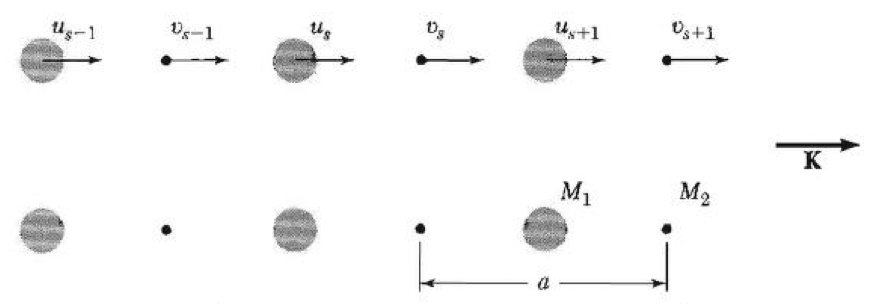
\includegraphics[scale=0.9]{atomic_chain.png}
\caption{Diatomic crystal structure showed in equilibrium positions with masses $M_1$ and $M_2$. The masses are connected to nearest neighbour by a spring constant C in the plane orthogonal to $K$. The atoms displacement of $M_1$ is denoted by $u_{s-1}$, $u_{s}$ and $u_{s+1}$ and $M_2$ by $\nu_{s-1}$, $\nu_{s}$ and $\nu_{s+1}$. The repeated distance is $a$ in the direction of wavevector $K$. Picture is lent from \cite{kittel2005}.}
\label{atomic_chain}
\end{figure}

A phononic bandgap can easily be modelled by an infinite 1D chain of diatomic crystal structure as illustrated in figure \ref{atomic_chain} with two atoms per unit cell \cite{kittel2005}. To see how we construct a basic bandgap we start by writing the equations of motion of such a system

\begin{align}
M_1\frac{d^2u_s}{dt^2} &= C\left( v_s + v_{s-1} - 2u_s \right) \\
M_2\frac{d^2v_s}{dt^2} &= C\left( u_s + u_{s+1} - 2v_s \right).
\end{align}
\noindent
Assuming plane wave solutions

\begin{align}
u_s &= ue^{isKa - i\omega t} \\
v_s &= ve^{isKa - i\omega t}.
\end{align}

we can solve these equation exactly for $\omega^2$. The corresponding dispersion relation can be seen in figure \ref{fig:bandgap}. We examine the limiting case at the upper boundary of the Brillouin zone, where $Ka = \pm \pi$ and find simple relations for the two branches in figure \ref{fig:bandgap}

\begin{align}
\omega_{acu}^2 & = \frac{2C}{M1} \\
\omega_{opt}^2 & = \frac{2C}{M2}.
\end{align}
\noindent
We can from these relations see that the size of the bandgap depends on ratio of the two masses.

\begin{figure}[H]
\centering
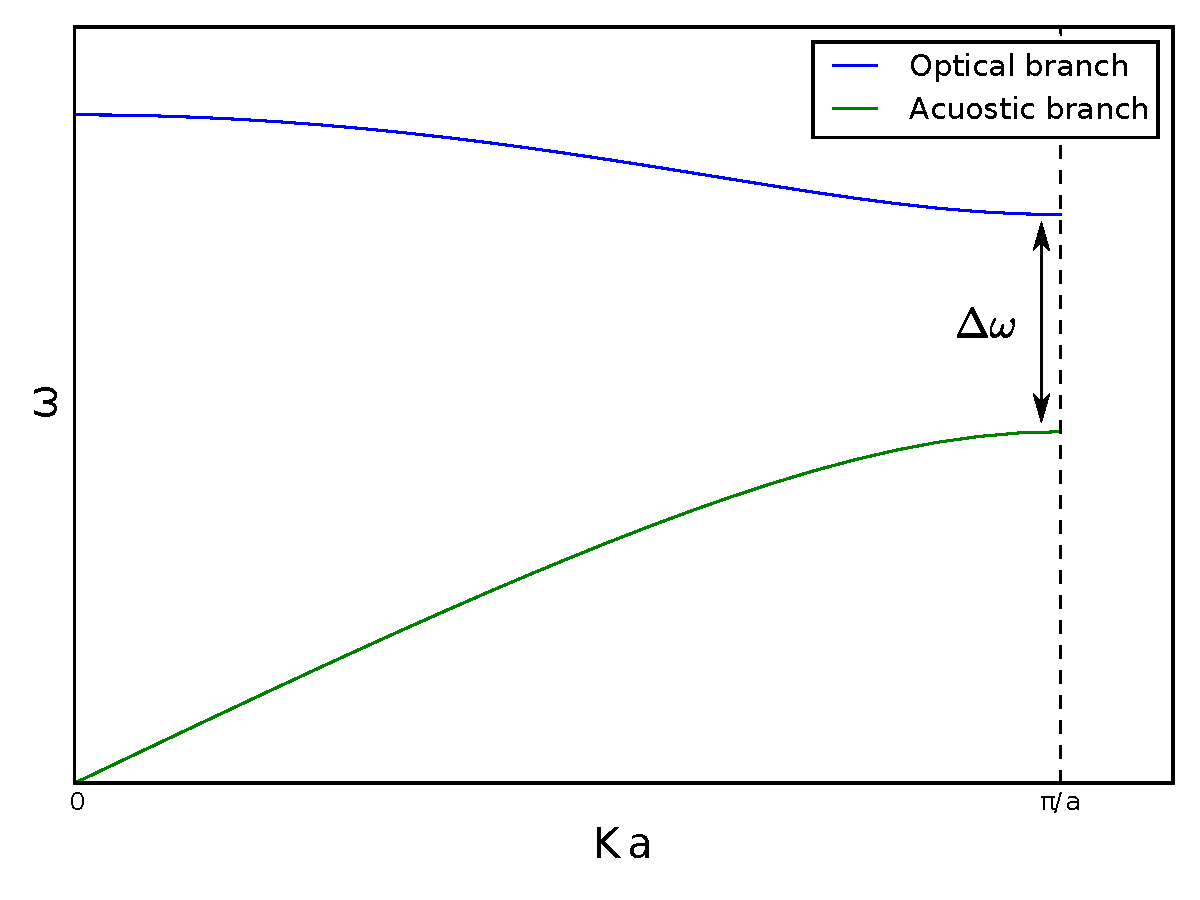
\includegraphics[scale=0.5]{bandgap.pdf}
\caption{Bands plotted for longitudinal modes. We see that we get a bandgap $\Delta\omega$ where no propagating modes can exist.}
\label{fig:bandgap}
\end{figure}

Calculating the dispersion relation of a real structure is however done numerically\footnote{Simulations are done using COMSOL Multiphysics by Yeghishe Tsaturyan. COMSOL is a commercial finite element analysis software.} and the resulting dispersion is, see figure \ref{fig:simulated_bandgap}.

\begin{figure}[H]
\centering
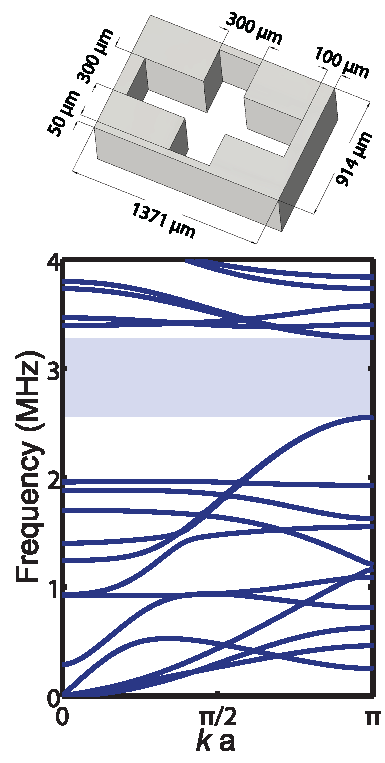
\includegraphics[scale=0.6]{bandgapery.pdf}
\caption{COMSOL simulated phononic structure \cite{tsaturyan2014}.}
\label{fig:simulated_bandgap}
\end{figure}
\noindent
To relate figure \ref{atomic_chain} to the actual structure in figure \ref{fig:simulated_bandgap}, see figure \ref{fig:spring_mass}.

\begin{figure}[H]
\centering
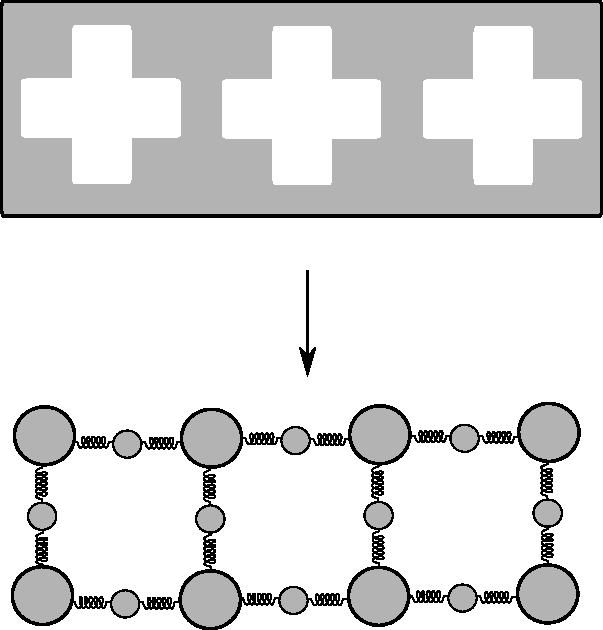
\includegraphics[scale=0.5]{spring_mass.pdf}
\caption{Our phononic structure ``translated" into the diatomic crystal model.}
\label{fig:spring_mass}
\end{figure}

\section{Cavity optomechanics}

\subsection{Optical cavity} \label{sec:opt_cav}
Cavities plays an important role in cavity optomechanics and we therefore need to expand our knowledge about them. The intention of this chapter is to introduce the building blocks for basic cavity theory. We shall only consider the Fabry-Perot geometry of a cavity, which consist of two opposing mirrors, normally introduced in textbooks as the Fabry-Perot etalon \cite{milonni2010}.

A cavity has several longitudinal resonances for which the angular frequency $\omega_n$ given by

\begin{equation}
\omega_n = 2\pi\cdot n\frac{c}{2L}, 
\end{equation}
\noindent
where $n$ is an integer mode number, $L$ is the cavity length and $c$ is the speed of light. The frequency spacing between two longitudinal modes is an important measure and is denoted as the free spectral range ($\mathrm{FSR}$) of the cavity, sometimes also written as $\omega_{\mathrm{FSR}}$ when given in angular frequency. It holds that

\begin{equation}
\omega_{\mathrm{FSR}} = 2\pi FSR  = \omega_{n+1} - \omega_n = 2\pi\frac{c}{2L}.
\end{equation}

Due to the finite properties of the mirrors such as reflectivities, transmittivities, internal absorption or scattering, cavities have a characteristic decay rate denoted $\kappa$. This leads us to the a second  useful quantity: the optical finesse $\mathcal{F}$, which is the average number of round-trips completed by a photon before departing from the cavity

\begin{equation}
\mathcal{F} = \frac{\omega_{FSR}}{\kappa}.
\end{equation}
\noindent
Finesse greater than one leads to an enhancement of the circulating intra-cavity power from the drive power. We have plotted the transmission through a Fabry-Perot cavity for multiple finesses in figure \ref{fig:trans_curve_finesse}. Achieving high finesse can be done by using mirrors with low losses and high reflectivities at the wanted wavelength. Cavity losses can generally be categorised by useful/good and bad losses. Input and output coupling typically being useful losses and the bad losses being internal loss, e.g. absorption or scattering. We therefore write

\begin{equation}
\kappa = \kappa_{ex} + \kappa_{0},
\end{equation}
\noindent
$\kappa_{ex}$ is the loss rate associated with input coupling and $\kappa_0$ is the sum of all remaining losses. Note that one could easily distinguish between more channels of decays, but for now this will do. We define a cavity coupling parameter $\eta_c$ like so

\begin{equation}
\eta_c = \frac{\kappa_{ex}}{\kappa}.
\end{equation}

There are in general three different cavity coupling regimes for cavities\footnote{The two others being: (1) undercoupled ($\kappa_0 > \kappa_{ex} \rightarrow \eta_c < \frac{1}{2}$) and (2) overcoupled ($\kappa_0 < \kappa_{ex} \rightarrow \eta_c > \frac{1}{2}$ )} \cite{schliesser2009}, but we will mainly use critical coupling ($\kappa_0 = \kappa_{ex} \rightarrow \eta_c = \frac{1}{2}$), since it is optimal for our application.
%A plot of cavity transmission of the different coupling regimes is shown in figure \ref{fig:trans_curve_reflections}.
%If only detecting in reflection the output coupling would be moved to $\kappa_0$.

\subsection{Cavity equations of motion} \label{sec:cav_eom}
In this subsection we will consider a one-dimensional field analysis of an optical cavity consisting of two mirrors separated by a fixed length $L$, and derive a cavity equation of motion. The Fabry-Perot cavity is driven by an incident electric field with amplitude $E_{in}$ and frequency $\omega_l$, through a single mirror port, from the left onto the first mirror. The mirrors are assumed to be thin lossless dielectric plates, with field reflection coefficients $r_{1,2}$ and transmission coefficients $t_{1,2}$. Note that the convention of reference plane is chosen such that the transmission becomes $it_{1,2}$. Both coefficients are considered to be real and fulfill $r_{1,2}^2 + t_{1,2}^2 = 1$. The intra-cavity will have a circulating field amplitude $E_{circ}$, the field moving in positive $z$ direction will be denoted $E_{circ}^+$, while the field propagating in opposite direction will be $E_{circ}^-$. It is the dynamics of the intra-cavity field that is of special interest. From the cavity we will have a reflected field $E_{ref}$ and transmitted field $E_{trans}$, see figure \ref{fig:E-field_model} for schematic layout.

\begin{figure}[H]
\centering
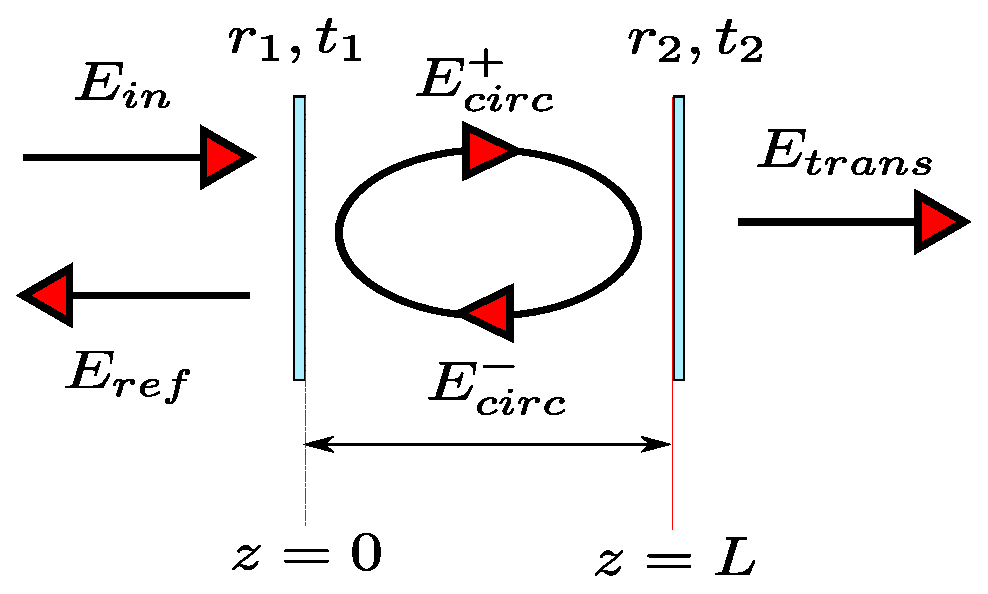
\includegraphics[scale=0.8]{E-field_model_edit.eps}
\caption{Fabry-Perot amplitude field analysis scheme, with input field $E_{in}$ onto the left mirror, cavity reflected field $E_{ref}$, intra-cavity fields $E_{circ}^{\pm}$ and cavity transmission $E_{trans}$. The cavity length is $L$ and $z = 0$ is placed at the inner surface of the incoupling mirror.}
\label{fig:E-field_model}
\end{figure}

We assume planar waves for the electric fields, where the index arrows shows propagation direction according to figure \ref{fig:E-field_model}

\begin{align}
E_{\rightarrow}(t, z) & = E_{\rightarrow}e^{i(\omega_l t + kz)} \\
E_{\leftarrow}(t, z) & = E_{\leftarrow}e^{i(\omega_l t - kz)}.
\end{align}
\noindent
It should be noted that the actual electric field is given by real part $\Re[E(z, t)]$, and that we omit the term $e^{i\omega_l t}$ in the calculations, since it drops out. We can then relate the input and output by a transfer matrix, keeping in mind that for a lossless mirror the matrix must be unitary

\begin{subequations}
\begin{align}
\begin{pmatrix}
E_{circ}^{+}(z = 0) \\
E_{ref}(z = 0)
\end{pmatrix}
 & =
\begin{pmatrix}
it_1 & r_1 \\
r_1 & it_1
\end{pmatrix} 
\begin{pmatrix}
E_{in}(z = 0) \\
E_{circ}^{-}(z = 0)
\end{pmatrix} \\
\begin{pmatrix}
E_{trans}(z = L) \\
E_{circ}^{-}(z = L)
\end{pmatrix}
 & =
\begin{pmatrix}
it_2 & r_2 \\
r_2 & it_2
\end{pmatrix}
\begin{pmatrix}
E_{circ}^{+}(z = L) \\
0
\end{pmatrix}.
\end{align}
\label{eq:E-field_transfer}
\end{subequations}
\noindent
This expression yields four coupled equations. Using that $E_{circ}^-$ in terms of $E_{circ}^+$ is $E_{circ}^- = r_2E_{circ}^+e^{2ikL}$ and taking the high-finesse limit $r_{1,2} \rightarrow -1$, we get the steady state solution for the circulating intra-cavity fields

\begin{equation}
E_{circ}^- = E_{circ}^+ = \frac{it_1 E_{in}}{1 - r_1r_2e^{2ikL}}.
\label{eq:high_finesse_approx}
\end{equation}
\noindent
The intra-cavity fields become equal in this limit and we can easily plot how the transmission through the cavity looks for different reflectivity coefficients of the mirrors, whilst keeping $r_1 = r_2$, see figure \ref{fig:trans_curve_finesse}.

\begin{figure}[H]
\centering
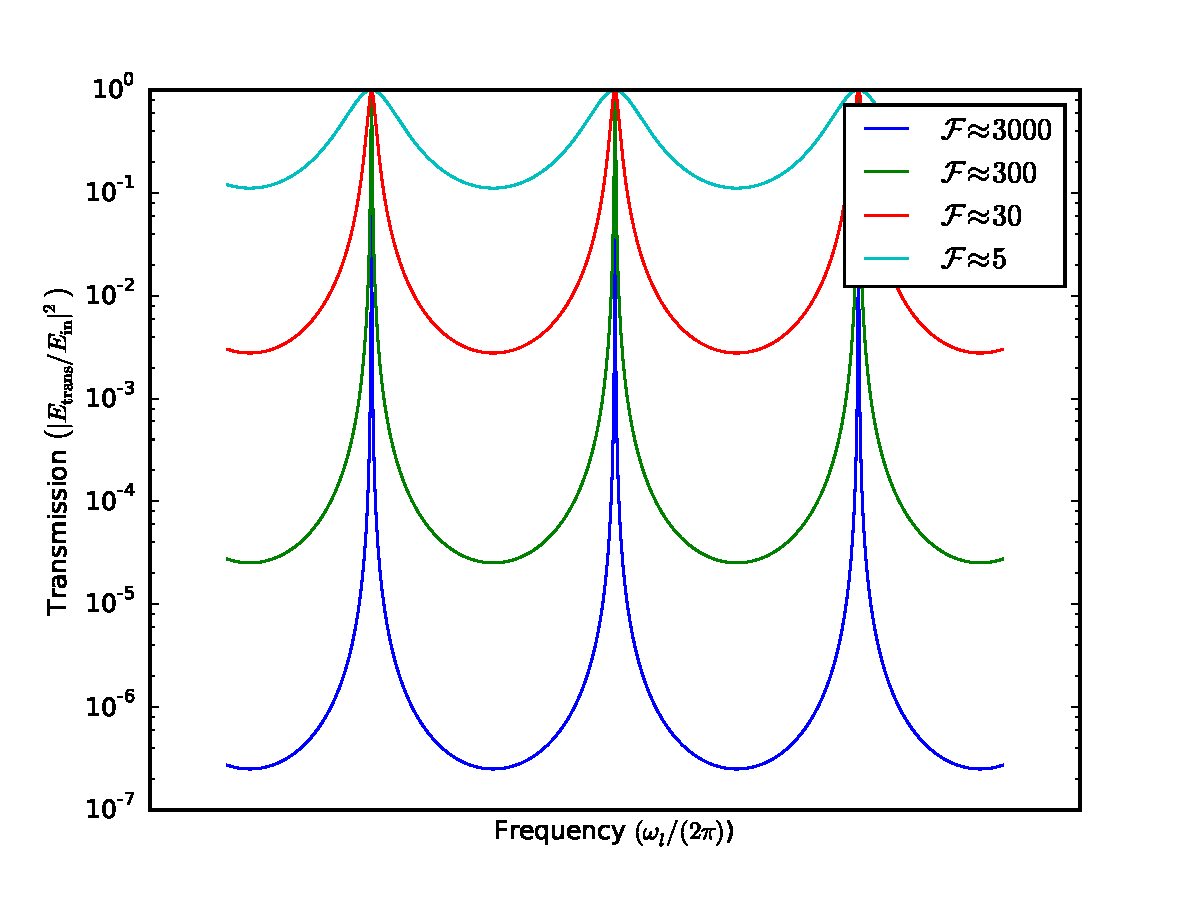
\includegraphics[scale=0.8]{cavity_model_fsr.pdf}
\caption{Transmissions through the cavity $\left| \frac{E_{trans}}{E_{in}} \right|^2$ whilst the laser frequency is changed for different finesses, i.e. reflection coefficients of the mirrors. Notice that the resonance peaks get broadened at lower finesse, this is due to an increase in $\kappa$, since it is the full-width-half-maximum of the lineshape. Another thing to notice is, that the spacing between each resonance corresponds to the $FSR$ of the cavity.}
\label{fig:trans_curve_finesse}
\end{figure}

%\begin{figure}[H]
%\centering
%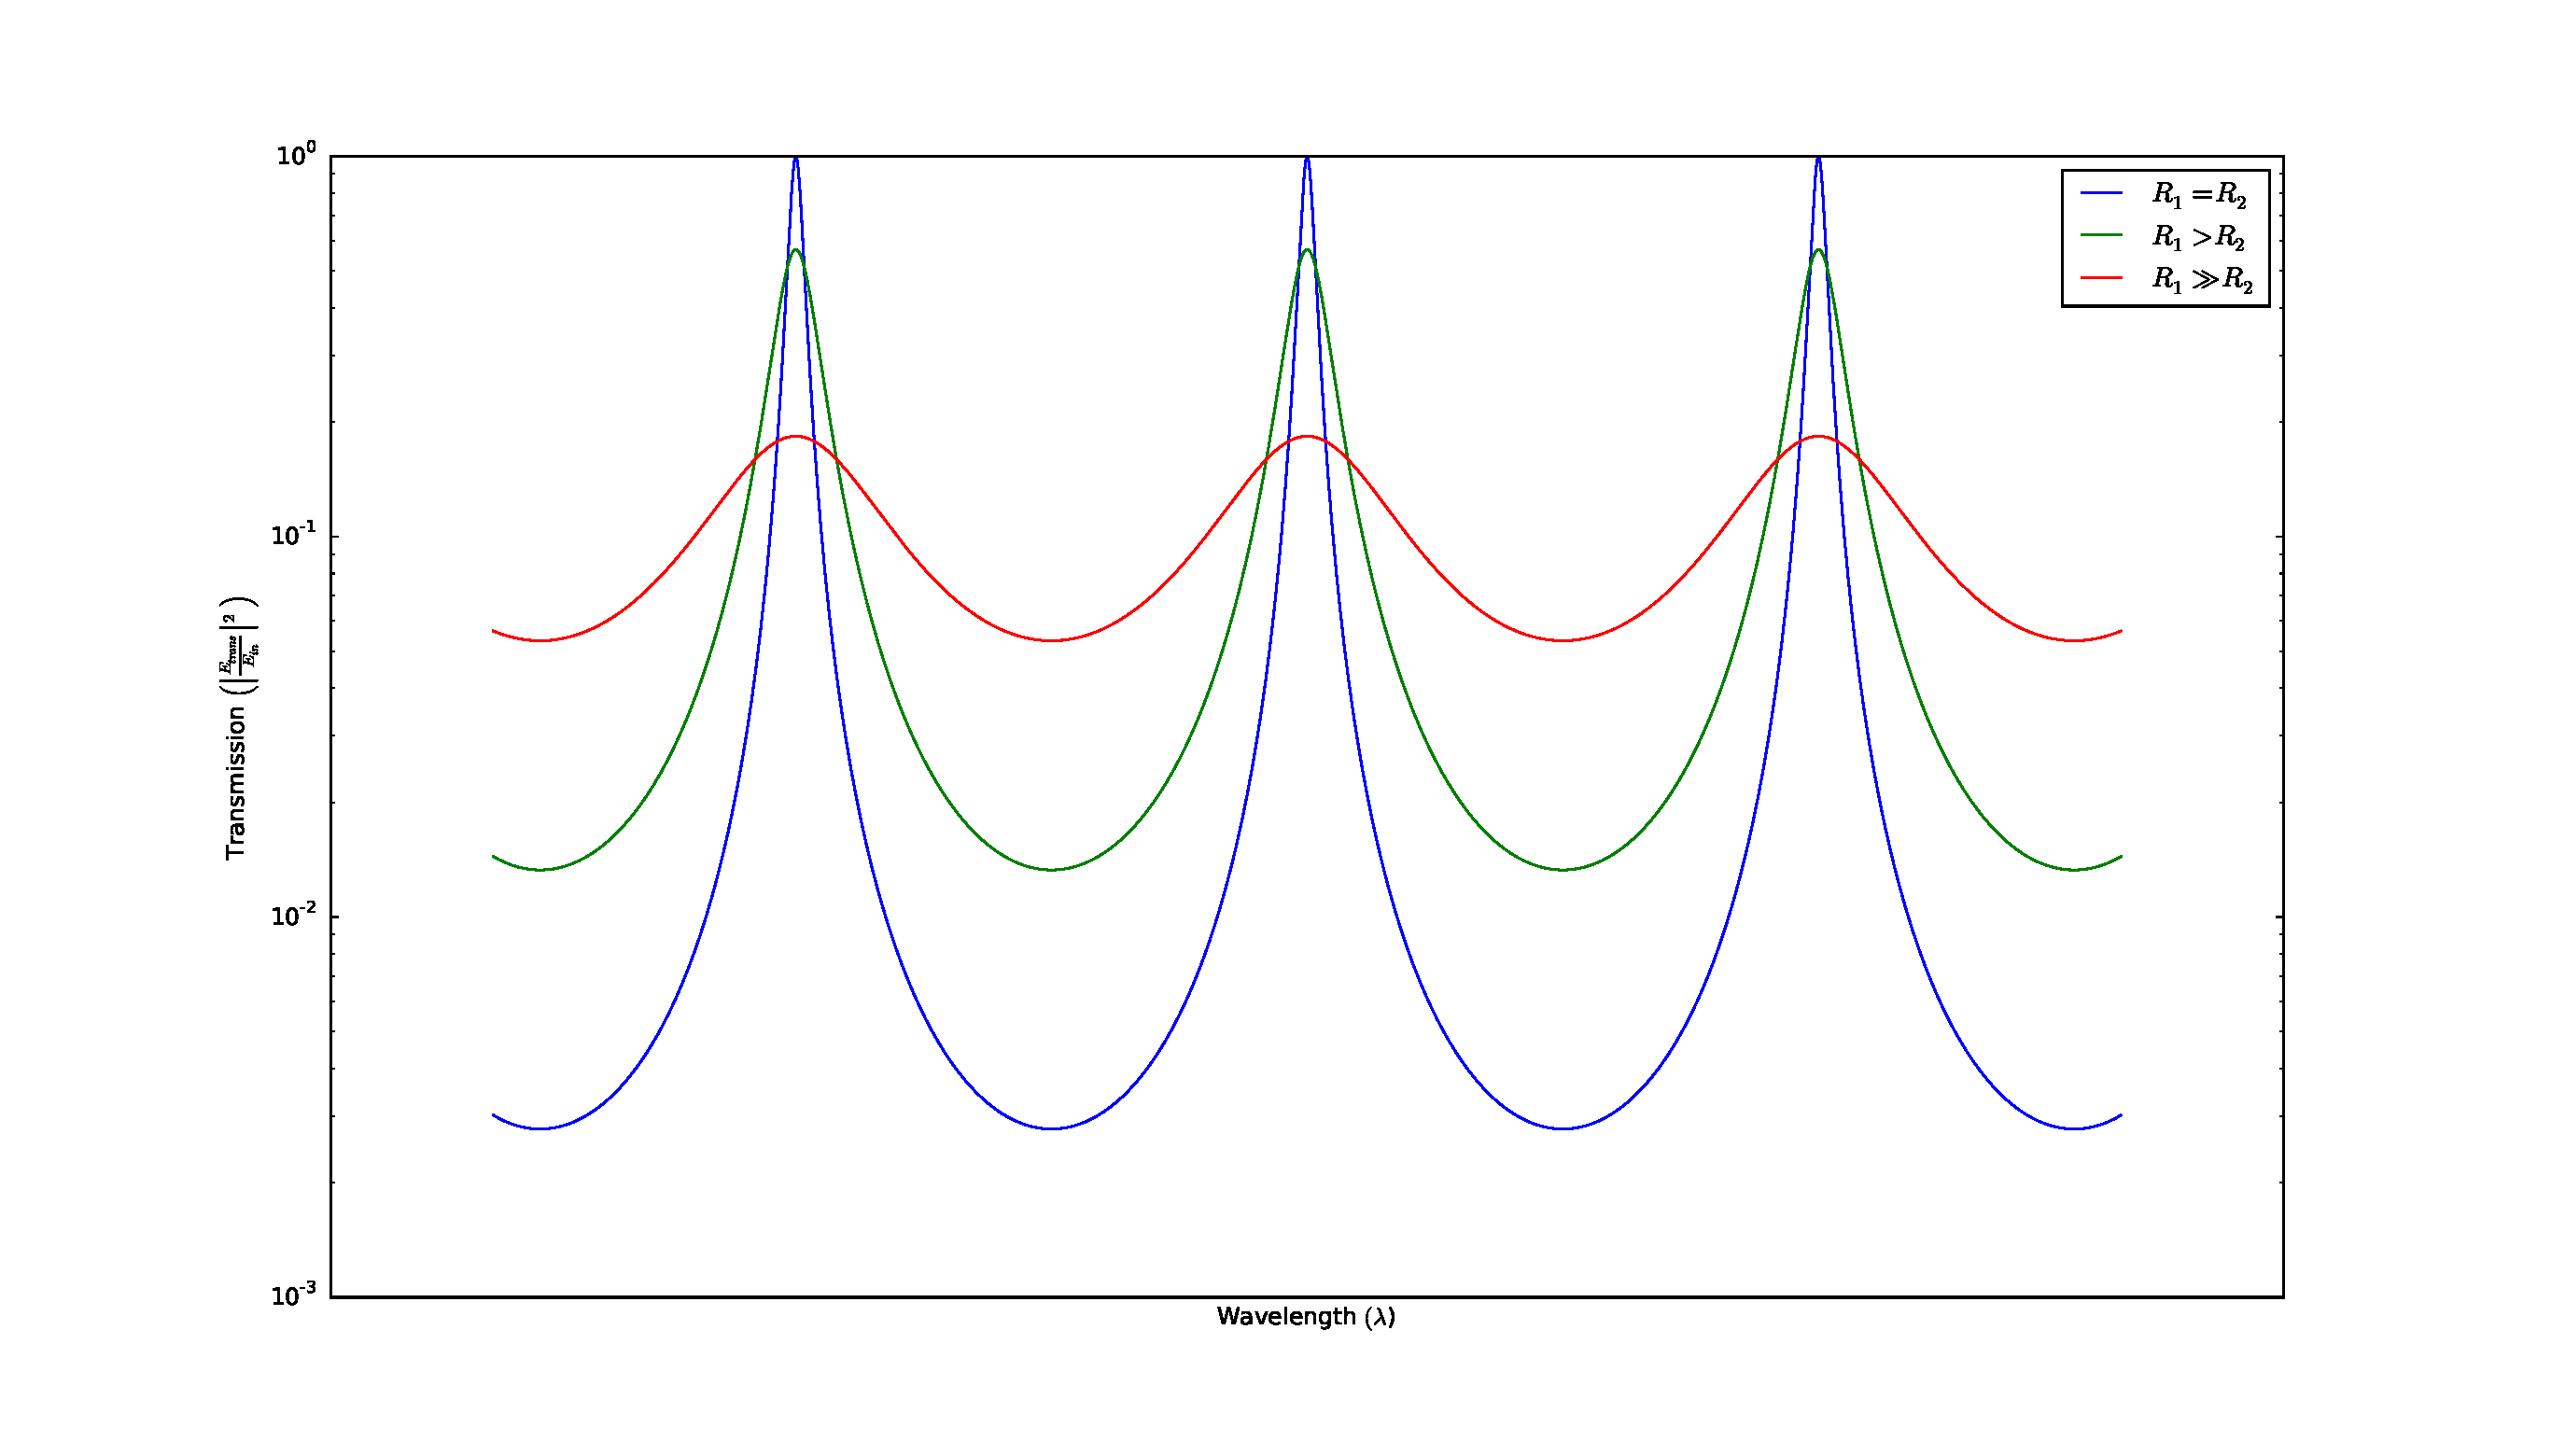
\includegraphics[scale=0.33]{trans_curve_reflections.eps}
%\caption{Bla bla}
%\label{fig:trans_curve_reflections}
%\end{figure}


We now depart from the steady state treatment and look at the slow build up and decay of the intra-cavity field. We allow for the amplitude of the fields to vary on a timescale much slower than the cavity round trip time $T_{rt} = \frac{2L}{c}$ the inverse of the free spectral range, and write

\begin{equation}
E_{circ}^+(t + T_{rt}) = it_1E_{in}(t) + r_1r_2e^{2ikL}E_{circ}^+(t),
\end{equation}
\noindent
where we have used the relation that the complex amplitude of a propagating field becomes multiplied by $r_1r_2e^{2ikL}$ after completing one round trip, thereby obtaining a relation for the time evolution of the circulating field: we obtain the differential equation

\begin{equation}
\frac{\mathrm{d}E_{circ}^+}{\mathrm{d}t} \approx \frac{E_{circ}^+(t + T_{rt}) - E_{circ}^+(t)}{T_{rt}} = \frac{it_1E_{in(t)}}{T_{rt}} + \left( r_1r_2e^{2ikL} - 1 \right)\frac{E_{circ}^+(t)}{T_{rt}}.
\label{eq:diff_field}
\end{equation}
\noindent
Previously we assumed high finesse limit to first order, but now we will include second order terms $r_1r_2 \approx 1 - (\frac{t_1^2}{2} + \frac{t_1^2}{2})$ and include low internal loss into the system. We model internal loss as a small imaginary component added to the regular wave number $k = \frac{\omega_L}{c}$:

\begin{equation}
e^{2ik'L} \approx \left(1 - \frac{\delta_{loss}}{2}\right)e^{2ikL}.
\end{equation}
\noindent
We now need to consider, what happens to the round trip phase $e^{2ikL}=e^{i\frac{\omega_L}{FSR}}$ close to cavity resonance $\omega_c$

\begin{equation}
e^{i\frac{\omega_L}{FSR}} \approx 1 - i\left( \frac{\omega_L - \omega_c}{FSR}\right).
\end{equation}
\noindent
We look back at equation \eqref{eq:high_finesse_approx} and remember that the magnitude of the intra-cavity fields traveling in both directions become equal in the high finesse limit. This means that the total circulating field $E_{circ}(t, z) = E_{circ}^{+}(t, z) + E_{circ}^{-}(t, z)$ becomes

\begin{equation}
E_{circ}(t, z) = 2E_{circ}(t)e^{i\omega_Lt}\sin(kz),
\end{equation}
\noindent
where $E_{circ}(t) \equiv iE_{circ}^+(t)$. We can now rewrite equation \eqref{eq:diff_field} in terms of $E_{circ}$ omitting second order terms

\begin{equation}
\frac{\mathrm{d}E_{circ}(t)}{\mathrm{d}t} \approx \frac{t_1E_{in}(t)}{T_{rt}} - E_{circ}(t)\left( \frac{t_1^2/2 + t_2^2/2 +\delta_{loss}/2}{T_{rt}} + i(\omega_L - \omega_c) \right).
\end{equation}
\noindent
This is basically the cavity equation of motion, but commonly we rescale the intra-cavity field with a factor of $E_{circ}(t)\sqrt{T_{rt}} = a(t)$. The newly defined variable is now normalized to the square root of the circulating intra-cavity energy; $a(t) = \sqrt{U_{circ}(t)}$, where the energy is related to the power by $U_{circ}(t) = T_{rt}P_{circ}(t)$. The rescaling is mainly done because the conversion to number of photons is easy, we just need to divide the energy with the energy of our photon $\hbar\omega_l$. Conversion to power, which we measure in the lab, is also easy. The equation of motion then reads

\begin{equation}
\dot{a}(t) = -\left(\frac{\kappa}{2} + i\Delta\right)a(t) + \sqrt{\kappa_1}E_{in}(t),
\label{eq:cavity_eom}
\end{equation}
\noindent
where the detuning is $\Delta = \omega_L - \omega_c$ and the sum of the decay rates is $\kappa = \kappa_1 + \kappa_2 + \kappa_{l}$, the transmission decay rates is $\kappa_{1,2} = \frac{t_{1,2}^2}{T_{rt}}$ and the internal loss rate is $\kappa_{l} = \frac{\delta_{loss}}{T_{rt}}$. We indentify the external losses $\kappa_{ex}$ with $\kappa_1$ and the rest with $\kappa_0$.

\subsection{Intra-cavity power}
Obtaining the cavity equation of motion is in it self valuable, but let us try to solve it and thereby get an expression relating the circulating intra-cavity power to the measured output power. To this end we will concentrate our effort on the transmission through the cavity.

We solve the cavity equation of motion \eqref{eq:cavity_eom} by taking its Fourier transform

\begin{equation}
a(\Omega) = \frac{\sqrt{\kappa_1}E_{in}(\Omega)}{\frac{\kappa}{2} + i(\Delta - \Omega)},
\end{equation}
\noindent
where $\Omega$ is an offset from the ``reference" frequency $\omega_L$. The solution is clearly dependent of its angular Fourier frequency component $\Omega$. If we consider the special case where our input field is just a constant, or in other words a monochromatic input field with frequency $\omega_L$, we can now write the input field as a constant and a delta function $E_{in} = E_0\delta(\Omega)$, where $\delta(\Omega)$ is the delta function. This means that the mean value of the rest of fields become just constants

\begin{equation}
\langle E_{in} \rangle = \frac{1}{2\pi}\int_{-\infty}^{\infty}d\Omega~E_0\delta(\Omega) = E_0.
\end{equation}
\noindent
It is of special interest to know the mean circulating intra-cavity power as a function of measured input or output power. This can now more or less easily obtained the circulating power by using the relation $\left| a \right|^2/T_{rt} = P_{circ}$

\begin{equation}
\langle P_{circ} \rangle = \frac{c}{2L} \left| a \right|^2 = \frac{\mathcal{F}\kappa}{2\pi\kappa_2}\langle P_{trans} \rangle,
\label{eq:cav_circ_pwr}
\end{equation}
\noindent
where is $\langle P_{trans} \rangle = \frac{4\kappa_1\kappa_2}{\kappa^2}\frac{1}{1 + \left(\frac{2\Delta}{\kappa}\right)^2}\langle P_{in} \rangle$. The mean circulating intra-cavity power is directly proportianal to the cavity finesse $\mathcal{F}$. To achieve high intra-cavity powers we must aim for as high finesse as possible, since optomechanical effect depend strongly on power.

\subsection{Cavity with moving boundary condition}
We now introduce a mechanical degree of freedom into our optical system and thereby realizing  an optomechanical system. In our case we will allow for the end mirror to move, for example like a harmonic oscillator, see figure \ref{fig:E-field_model_moving}. These kinds of systems come in many various constellations, e.g. microtoriods \cite{weis2010} and the photonic crystal nano beam \cite{chan2011}. Both of these systems have produced great results, such as ground state cooling and and optomechanical induced transparency. For an extended overview of different systems see \cite{aspelmeyer2014}.

\begin{figure}[H]
\centering
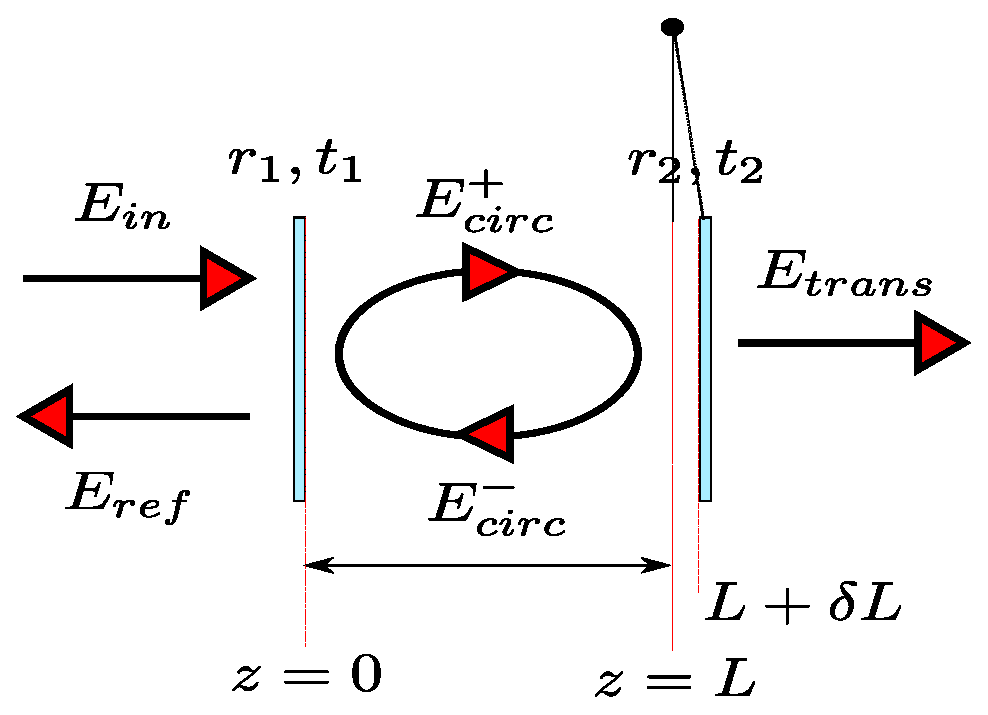
\includegraphics[scale=0.8]{E-field_model.eps}
\caption{We allow for a small pertubation to the cavity length $\delta L$. Here the mechanical degree of freedom is the not canonical pendulum, for visual purposes. The cannonical}
\label{fig:E-field_model_moving}
\end{figure}

We want to investigate the effect of a movable end mirror in a cavity. We introduce a displacement of the end mirror as a small perturbation $\delta L$ to the otherwise fixed cavity length $\tilde{L} = L + \delta L$ and assume that $\delta L \ll L$. The perturbation changes our cavity resonance frequency $\omega_c \rightarrow \omega_c^\prime$.

\begin{equation}
\omega_c^\prime = 2\pi\frac{c}{2\left( L + \delta L \right)}n
\end{equation}
\noindent
a linearization of the equation above yields

\begin{equation}
\omega_c^\prime \approx \omega_c - \frac{\omega_c}{L}\delta L
\label{eq:opt_coup}
\end{equation}
\noindent
This result is for the special case of a Fabry-Perot cavity. A more general way of writing the mechanical induced modulation of the cavity resonance would be, again only keeping the linear term

\begin{equation}
\omega_c^\prime(z) \approx \omega_c + \delta z\frac{\partial\omega_c}{\partial z}\bigg|_{z = z_0}
\end{equation}
\noindent
We normally define the optical frequency shift per displacement as $G \equiv \left|\frac{\partial\omega_c}{\partial z}\right|$. We easily recognize that for a Fabry-Perot cavity it is just the cavity resonance divided by the cavity length $G_{FP} = \frac{\omega_c}{L}$ as seen in equation \eqref{eq:opt_coup}. Note that $G_{FP}$ is inversely proportional to the cavity length $L$, so smaller cavity length are preferred.

We deliberately avoided using the term ``optomechanical coupling" in this section, since it is the cause of confusion in this field of study\footnote{Do not say I did not warn you!}.

\subsection{Classical cavity optomechanics} \label{sec:clas_opt_mech}
\subsubsection{Radiation pressure force}
We now wish to couple the movable mirror motion to the amplitude of the intra-cavity field. The coupling is mediated by a radiation pressure force $F_{rad}$ experienced by the movable mirror. A single reflected photon transfers the momentum onto a mirror

\begin{equation}
\Delta p = \frac{2h}{\lambda},
\end{equation}
\noindent
where $h$ Planck's unreduced constant and $\lambda$ the photon wavelength. Our radiation pressure force of $n$ number photons inside a cavity $F_{rad}$ can then be written as

\begin{equation}
F_{rad} = \frac{\Delta p}{T_{rt}}n = \frac{2\hbar k}{T_{rt}}n = \frac{U_{circ}}{L} = \frac{2P_{circ}}{c},
\label{eq:rad_force}
\end{equation}
\noindent
where $T_{rt}$ again is the round trip time. We assume to be in vacuum such that the phase velocity is equal to $c$.% and the energy $U_{circ} = \frac{\hbar k n}{c}$.

The dynamics of a system that couples an optical field with a mechanical degree of freedom depends critically on the optical frequency shift per displacement, namely $G$. Initially it might not be apparent from equation \eqref{eq:rad_force}, but rewriting the radiation pressure force in terms of work done on the cavity by a small displacement $x$

\begin{equation}
F_{rad} = -\frac{d U_{mech}}{dx} = \frac{d U_{circ}}{dx},
\label{eq:rad_force_work}
\end{equation}
\noindent
where $U_{mech}$ is the mechanical energy. Note that the cavity length now at any particular time is $L + x$. Applying the chain rule to equation \eqref{eq:rad_force_work},

\begin{equation}
\frac{d U_{circ}}{dx} = \frac{d U_{circ}}{dL}\frac{d L}{d\omega_c}\frac{d\omega_c}{dx}.
\end{equation}
\noindent
One can argue that $\frac{d U_{circ}}{dL} = \frac{U_{circ}}{L}$, $\frac{dL}{d\omega_c} = \frac{-\pi c}{\omega_c^2}$ and we previously defined $G = \frac{d\omega_c}{dx}$. We can now see the direct relation between radition pressure force and $G$

\begin{equation}
F_{rad} = -G\frac{U_{circ}}{\omega_c}.
\end{equation}
\noindent
Our modified equations of motion for the cavity field and mechanics become

\begin{equation}
\dot{a}(t) = -\left( + \frac{\kappa}{2} + i(\Delta - Gx(t)) \right)a(t) + \sqrt{\kappa_1}E_{in},
\end{equation}
\noindent
and
\begin{equation}
\frac{1}{m}\left( F_{th}(t) + F_{rad} \right) =\ddot{x}(t) + \Gamma_m\dot{x}(t) + \Omega_m^2x(t).
\end{equation}
\noindent
The equations of motion for the cavity field and mirror motion are coupled through $F_{rad}$ with $U_{circ} = \left| a(t) \right|^2$ see section \ref{sec:cav_eom}.

\subsubsection{Dynamical backaction: Optical spring and damping}
We can approximate a solution by adding a small perturbation to each variable around their steady-state, e.g. $x(t) =  \langle x \rangle + \delta x(t)$. This is done for each of the variables except for the input field, since it is a monochromatic laser field that has no time dependent small variation i.e. $\delta E_{in}(t) = 0$. That means that we neglect quantum noise. We assume that the cavity resonance is only changed by a small fraction of the cavity linewidth, like so $\frac{G\delta x}{\kappa} \ll 1$, which means that the small perturbation assumption also holds for the intra-cavity field. Our linearized coupled equations of motion to first order ($\delta a/\langle a \rangle$ and $\delta x/\langle x \rangle$) become

\begin{align}
\delta \dot{a}(t) = -\left(\frac{\kappa}{2} + i\bar{\Delta}\right)\delta a(t) - iG\delta x(t)\langle a \rangle \label{eq:a_fluc} \\
\frac{1}{m}\left( \delta F_{th}(t) + \delta F_{rad}(t) \right) = \delta \ddot{x}(t) + \Gamma_m\delta\dot{x}(t) + \Omega_m^2x(t) \label{eq:x_fluc},
\end{align}
\noindent
where $\bar{\Delta} = \omega_L - \omega_c -G\langle x \rangle$ is a new modified detuning.

Let us take a closer look at the fluctuating part of the radiation pressure force. To first order in $\delta a(t)$, i.e. omitting $\langle F_{rad}\rangle$ and remembering that the intra-cavity field amplitude $a(t)$ is a complex number

\begin{equation}
\delta F_{rad} = F_{rad} - \langle F_{rad}\rangle = - \frac{G}{\omega_c}\left( \langle a \rangle \delta a^*(t) + \delta a(t) \langle a \rangle^* \right),
\end{equation}
\noindent
where $\delta a^*(t)$ and $\langle a \rangle^*$ are just the complex conjugates. To clarify the dynamics of the effects of the radiation pressure force on the mirror displacement, we need to represent the equations of motion in the Fourier domain, $\mathcal{F}[\delta a(t)]$ and $\mathcal{F}[\delta x(t)]$, which is basically the same as solving the differential equations \eqref{eq:a_fluc} and \eqref{eq:x_fluc}

\begin{align}
\delta a(\Omega)\left(\frac{\kappa}{2} + i(\Delta - \Omega)\right) = -iG\delta x(\Omega) \langle a \rangle \\
\frac{1}{m}\left( \delta F_{th}(\Omega) + \delta F_{rad}(\Omega) \right) = -\Omega^2\delta x(\Omega) - i\gamma\Omega\delta x(\Omega) + \Omega_m^2\delta x(\Omega).
\end{align}
\noindent
Taking a second look at the fluctuating part of the radiation pressure force in the Fourier domain,

\begin{equation}
\begin{split}
\delta F_{rad}(\Omega) & = -\frac{G}{\omega_c}(\langle a \rangle\delta a^*(\Omega) + \langle a \rangle^*\delta a(\Omega)) \\
 & = \frac{G^2 \langle U_{circ} \rangle}{\omega_c}(A_+(\Omega) + A_-(\Omega))\delta x(\Omega),
 \label{eq:rad_force_fluc}
\end{split}
\end{equation}
\noindent
where $A_{\pm}(\Omega) \equiv \frac{\pm i}{\frac{\kappa}{2} \mp i(\Delta - \Omega)}$ is denoted as the strength of the generated sidebands of the intra-cavity field at $\pm\Omega$ by the moving mirror.

We see that the radiation pressure force fluctuations in equation \eqref{eq:rad_force_fluc} depends on the static radiation pressure force $\langle \delta F_{rad} \rangle = -\frac{G}{\omega_c}\langle U_{circ} \rangle$, the cavity frequency fluctuations $G\delta x(\Omega)$ driven by the moving mirror and $(A_+(\Omega) + A_-(\Omega))$ being the dynamic response of the intra-cavity energy to resonance fluctuations. An important note is that the response term contains an imaginary component related to the finite build-up time of the cavity field, as a consequence  $\delta F_{rad}(\Omega)$ will have components both oscillating in phase with the mirror position $\propto \delta x(\Omega)$ {\it and} mirror velocity $\propto [\delta \dot{x}](\Omega)$. We call these effects the optical spring $k_{opt}$ and optical damping $\Gamma_{opt}$, because of the analogy to their classical counter parts.

We then express the newly introduced effect of the radiation pressure force fluctuations on the dynamics of the mirror motion by defining an effective mechanical susceptibility $\chi_{eff}(\Omega) \equiv \frac{\delta x(\Omega)}{\delta F_{th}(\Omega)}$;

\begin{equation}
\begin{split}
\chi_{eff}^{-1}(\Omega) & = m(-\Omega^2 -i\Gamma_m\Omega + \Omega_m^2) - \frac{\delta F_{rad}}{\delta x(\Omega)} \\
 & = m(-\Omega^2 + (\Delta\Omega_{opt}(\Omega) + \Omega_m)^2 -i\Omega(\Gamma_m + \Gamma_{opt}(\Omega))),
\end{split}
\end{equation}
\noindent
where $\Delta\Omega_{opt}(\Omega) = k_{opt}(\Omega)/(2m\Omega_m)$ is the effect of the optical spring shift on the mechanical frequency, i.e. hardening or softening of the spring. Our optically induced effects become

\begin{equation}
k_{opt}(\Omega) \equiv -\operatorname{Re}\left[{\frac{\delta F_{rad}(\Omega)}{\delta x (\Omega)}}\right],
\end{equation}
\noindent
and
\begin{equation}
\Gamma_{opt}(\Omega) \equiv -\operatorname{Im}\left[{\frac{\delta F_{rad}(\Omega)}{\delta x (\Omega)}}\right]\frac{1}{m\Omega}.
\end{equation}
\noindent
If we assume sufficiently weak laser drive and  radiation pressure force, i.e. $\kappa \gg G,\Gamma_{eff}$, where $\Gamma_{eff} = \Gamma_m + \Gamma_{opt}$ is  the effective damping rate, we can approximate the optically induced effects in the unperturbed oscillation frequency as $\chi_{eff}^{-1}(\Omega = \Omega_m)$, because it is the only Fourier component which gives a contribution in this limit.

\begin{equation}
\Delta\Omega_{opt}(\Omega_m) = \frac{1}{2m\Omega_m}\frac{G^2\langle U_{circ} \rangle}{\omega_c}\left( \frac{\Delta - \Omega_m}{\left(\frac{\kappa}{2}\right)^2 + (\Delta - \Omega_m)^2} + \frac{\Delta + \Omega_m}{\left(\frac{\kappa}{2}\right)^2 + (\Delta + \Omega_m)^2} \right)
\end{equation}

\begin{equation}
\Gamma_{opt}(\Omega_m) = \frac{\kappa}{2m\Omega_m}\frac{G^2\langle U_{circ} \rangle}{\omega_c}\left( \frac{1}{\left(\frac{\kappa}{2}\right)^2 + (\Delta + \Omega_m)^2} - \frac{1}{\left(\frac{\kappa}{2}\right)^2 + (\Delta - \Omega_m)^2} \right).
\label{eq:gamma_opt}
\end{equation}
\noindent
An easy way to inspect the equations above is by choosing a detuning from our cavity resonance $\Delta \approx \pm \Omega_m$, since the equations simplify greatly in this limit. For positive detuning $\Delta \approx \Omega_m$, i.e. blue detuning, we get a positive optically induced frequency shift and a negative damping contribution to the effective damping coefficient. If the effective damping becomes negative, it leads to an instability in the system. But if we red detune by $\Delta \approx -\Omega_m$, things get more interesting, in partiular that we get an positive optically induced damping contribution and a negative frequency shift. This is known as cooling by dynamical backaction\footnote{Previously called the Braginsky effect.} of the mechanical mode. In other words $\Gamma_{opt}(\Omega)$ is the rate of transfer of mechanical energy into electromagnetic energy. One question quickly jumps to ones mind: by how much can we cool the mechanical mode? To answer this we shall write out the modified power spectral density for the thermal fluctuations and integrate over it to obtain an effective temperature $T_{eff}$;

\begin{equation}
S_{xx}(\Omega) = \left| \chi_{eff}(\Omega) \right|^2S_{FF}(\Omega).
\end{equation}
\noindent
We can from this expression derive the effective temperature of the reduced mechanical vibrational energy
%If we dissipate mechanical energy into the eletromagnectic energy faster than thermal excitation from the coupled thermal bath $\Gamma_{m} < \Gamma_{opt}$ it leads to optical cooling, by reducing the mechanical vibrational energy

\begin{equation}
T_{eff} = \frac{m_{eff}}{k_B}\Omega_m^2\int_0^\infty \frac{d\Omega}{2\pi}S_{xx}(\Omega) \approx \frac{\Gamma_m}{\Gamma_m + \Gamma_{opt}}T_{bath}.
\end{equation}
\noindent
Since $\Gamma_{opt}$ can get arbitrary large, due to $\langle U_{circ} \rangle$ we can seemingly cool all the way to $T_{eff} \approx 0$ or a zero phonon occupancy. End of story, right? Well, not exactly! As we will show later, in the quantum picture, there are limits to how well we can cool. In this model we did not for example take into account fluctuations in the input field. What we just derived is know as dynamical backaction, i.e. fluctuations in the intra-cavity field caused by fluctuation of the mechanical oscillator.

\subsection{Sideband regimes}
In the previous section we mentioned the red detuning away from the cavity resonance leads to optical cooling effects. We normally differ between the optimal cooling regime, i.e. resolved sidebands, and the less optimal cooling regime, i.e. unresolved sidebands. As shown in the section above vibrating mirror causes scattering of the cavity fields into sidebands $A_{\pm}$. We can use the cavity to either amplify or suppress/filter out the generated sidebands at frequency $\Omega_m$. The resolved sideband regime is reached when your cavity linewidth becomes much smaller than the mechanical resonance, i.e. $\kappa \ll \Omega_m$, as shown in figure \ref{fig:resolved_sb}. If this criteria is fulfilled the cavity can only support one generated sideband and therefore suppresses the other sideband.

\begin{figure}[H]
\centering
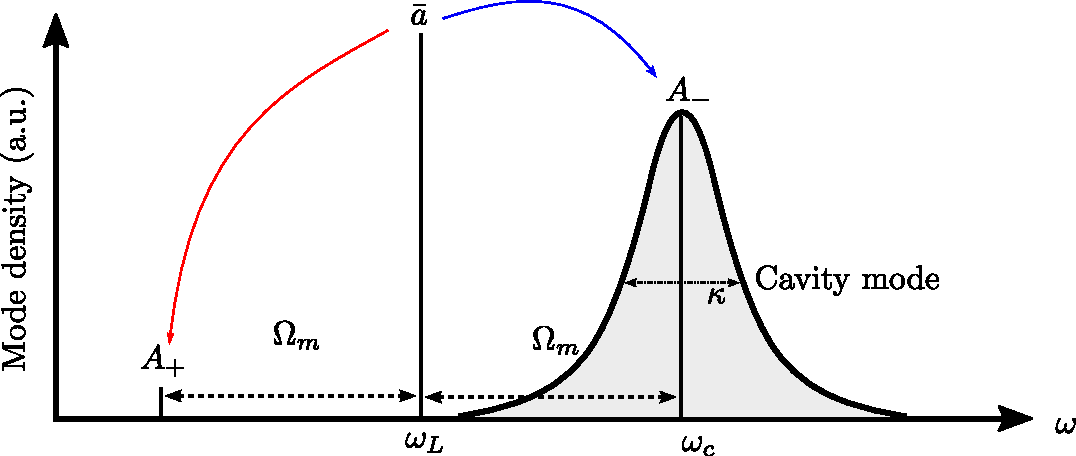
\includegraphics[scale=0.8]{resolved_sb.pdf}
\caption{Scatter picture of optimal cooling in the resolved sidebands regime. The cavity mode only supports the $A_-$ mode at frequency $\Omega_m$ detuned from the carrier and filters out the rest.}
\label{fig:resolved_sb}
\end{figure}

Moving on to describing the unresolve sidebands regime, i.e. $\Omega_m \ll \kappa$. This regime is as mentioned less optimal for cooling, since the cavity linewidth is now much larger than the mechanical resonance as shown in figure \ref{fig:unresolved_sb}. The cavity can now support both sidebands at the same time, so heating and cooling is present at the same time.

\begin{figure}[H]
\centering
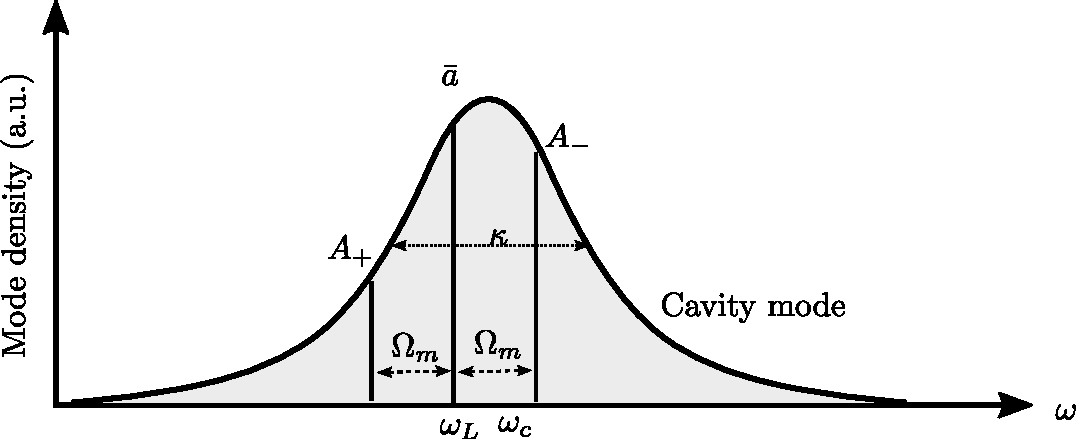
\includegraphics[scale=0.8]{unresolved_sb.pdf}
\caption{Scattering picture in the unresolve sidebands regime. The cavity resonance is now much broader than the mechanical resonance.}
\label{fig:unresolved_sb}
\end{figure}

\subsection{Optical properties of the membrane}
The dielectric SiN membranes have extraordinary optical properties such as low absorption \cite{Wilson2011}, but it lacks a bit in reflectivity. The dielectric membrane with thickness $d$ has the electric field reflectivity coefficient $r_m$ and transmission coefficient $t_m$ \cite{jayich2008, Wilson2011}

\begin{align}
  \label{eq:mem_opt_prop}
  r_m & = \frac{(n^2 -1)\sin(knd_m)}{2in\cos(knd) + (n^2 +1)\sin(knd)} \\
  t_m & = \frac{2n}{2in\cos(knd) + (n^2 +1)\sin(knd)},
\end{align}
\noindent
where $n$ is the index of refraction of the dielectrics and $k$ is the wavenumber of the light incident on the membrane. In figure \ref{fig:mem_prop} we show the reflectivity coefficient $r_m$ as a function of refractive index $n$, which is also equivalent to increasing the thickness $d$. We also plot $r_m$ for a realistic index of refraction $n = 2$ \cite{Wilson2011} and vary the wavelength in figure \ref{fig:mem_prop}.

\begin{figure}[H]
\centering
    \begin{subfigure}[b]{0.49\textwidth}
    \centering
    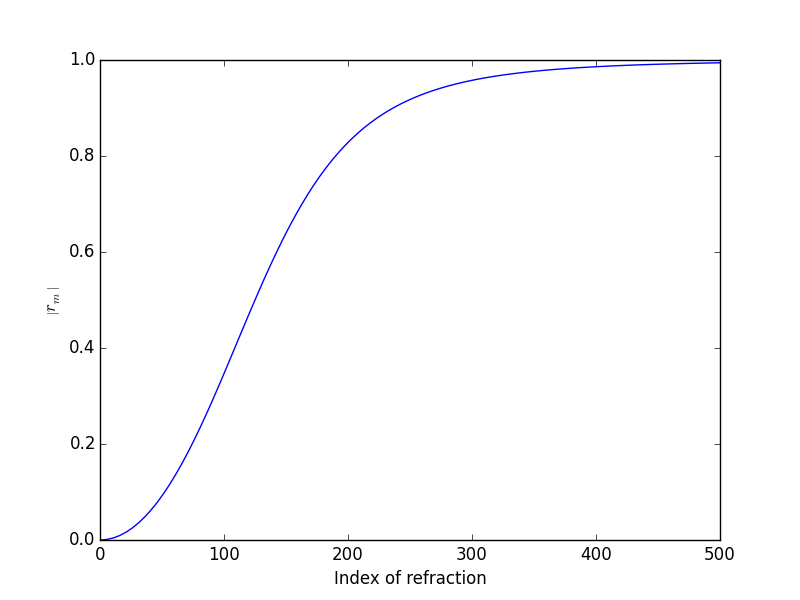
\includegraphics[width=\textwidth]{mem_ref_vs_index_of_refrac.png}
    \caption{}
    \label{fig:mem_ref_refrac}
    \end{subfigure}
    \hfil
    \begin{subfigure}[b]{0.49\textwidth}
    \centering
    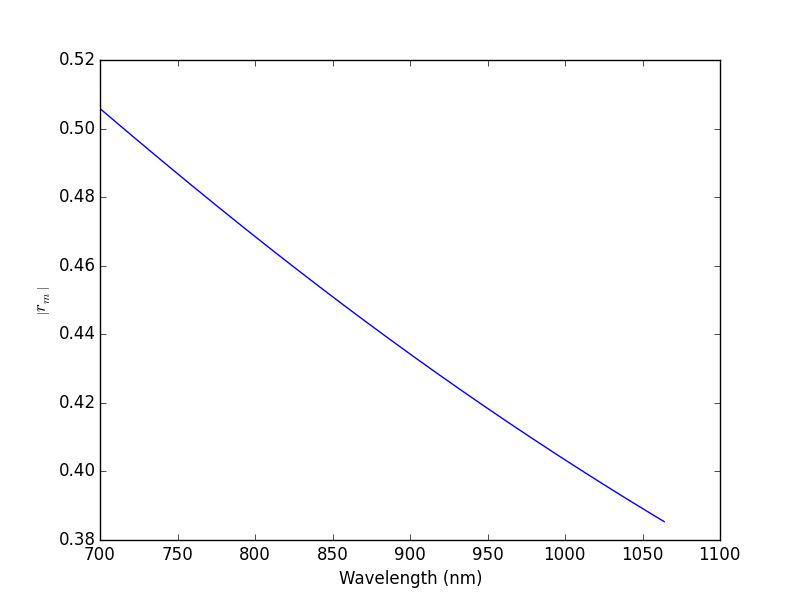
\includegraphics[width=\textwidth]{mem_ref_vs_wavelength.png}
    \caption{}
    \label{fig:mem_ref_wavelength}
    \end{subfigure}
\caption{(a) Membrane reflectivity coefficient $r_m$ as a function of index of refraction $n$. (b) Reflectivity coefficient $r_m$ as we change the wavelength of the light for fixed index of refraction $n = 2$.}
\label{fig:mem_prop}
\end{figure}

\subsection{Membrane-in-the-middle system}
Most optomechanical systems try to minimize losses, both mechanical and optical. Another parameter that is of particular interest is mass or rather effective mass of the mechanical oscillator, because smaller masses enhances the interaction between optical and mechanical degree of freedom. It can be thought of as a single photon having a higher impact, because of the smaller effective mass. But small mass and great optical properties, such as high reflectivity, do not always commute. ``Nano/micro" membranes do not possess a high enough reflectivity, such that one can reach the high finesse limit with only a high reflective mirror and a membrane. Normally membranes do not have reflectivities $\left| r_m \right|^2$ exceeding 0.5, even though attempts are being made by stacking them in layers. This kind of ruin the plan of creating an optomechanical system with low optical loss. But enclosing an ultra-thin dielectric film between two mirrors of an already high finesse optical cavity solves the problem. We call it the membrane-in-the-middle (or MIM) system \cite{thompson2008,jayich2008} and is depicted in figure \ref{fig:transfer_model}.
The membrane-in-the-middle system is one way to achieve a trade-off between great mechanical performance and low optical loss. Mirrors which enable high finesse are commercially available at finesses $\mathcal{F} > 10^6$ and mechanical resonators are also commercially available \cite{jayich2008} or can be fabricated ``in-house" with very high quality factors $Q > 10^6$ \cite{tsaturyan2014}.

\subsection{Transfer matrix model} \label{sec:trans_matrix}
In section \ref{sec:cav_eom} we presented an amplitude field analysis of the canonical optomechanical system. The scope of this chapter is to apply the model to, in our case, a more appropriate system, i.e. the    membrane-in-the-middle, and see how the medium inside the cavity changes the cavity resonance as a function of membrane position $x$. We follow the approach presented in \cite{jayich2008, Wilson2011}. Our amplitude fields of the system are presented to the right in figure \ref{fig:transfer_model}.

\begin{figure}[H]
\centering
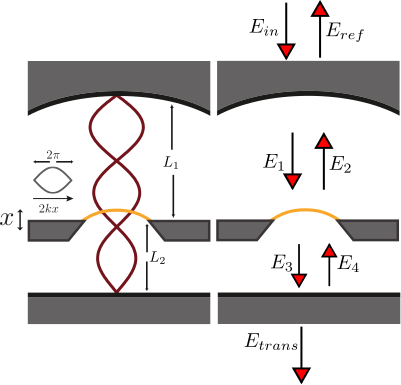
\includegraphics[scale=0.8]{transfer_matrix.png}
\caption{Two identical cavities: The left cavity shows how the membrane position $x$ is placed in the standing wave ``bubble" $2kx$ and the right cavity shows the schematic of the subcavity amplitude field analysis.}
\label{fig:transfer_model}
\end{figure}

The Fabry-Perot cavity is now divided into two sub-cavities of lengths $L_1$ and $L_2$, respectively (left and right sides) separated by a membrane with amplitude reflection coefficient $r_m$ and transmission $t_m$. We apply the same method as in section \ref{sec:cav_eom} and get a set of coupled equations

\begin{subequations}
\begin{align}
E_1 & = it_1E_{in} + r_1E_2e^{ikL_1} \\
E_2 & = r_mE_1e^{ikL_1} + it_mE_4e^{ikL_2} \\
E_3 & = it_mE_1e^{ikL_1} + r_mE_4e^{ikL_2} \\
E_4 & = r_2E_3e^{ikL_2} \\
E_{refl} & = it_1E_2e^{ikL_1} + r_1E_{in} \\
E_{trans} & = it_2E_3e^{ikL_2}
\end{align}
\end{subequations}
\noindent
We can obtain a solution for the variation in cavity resonance modulated by membrane position by writing up the closed system, i.e. excluding reflection and transmission, and find its eigenfrequencies

\begin{equation}
\begin{pmatrix}
E_{in} \\
E_{1} \\
E_{2} \\
E_{3} \\
E_{4}
\end{pmatrix}
  =
\begin{pmatrix}
1 & 0 & 0 & 0 & 0\\
it_1 & 0 & r_1e^{ikL_1} & 0 & 0 \\
0 & r_me^{ikL_1} & 0 & 0 & it_me^{ikL_2} \\
0 & it_me^{ikL_1} & 0 & 0 & r_me^{ikL_2} \\
0 & 0 & 0 & r_2e^{ikL_2} & 0 \\
r_1 & 0 & it_1e^{ikL_1} & 0 & 0 \\
0 & 0 & 0 & it_2e^{ikL_2} & 0
\end{pmatrix} 
\begin{pmatrix}
E_{in} \\
E_{1} \\
E_{2} \\
E_{3} \\
E_{4}
\end{pmatrix} \\
\label{eq:transfer_matrix}
\end{equation}
\noindent
As an approximation the mirrors will be assumed to yield high finesse $r_{1,2} \approx 1$, also we will neglect absorption of the membrane, i.e. the imaginary part of the index of refraction is set to zero; $\Im[n] = 0$. We will also assume that the membrane is placed in the middle such that the subcavity lenghts become equal, we rewrite the cavity length $L_1 \rightarrow L + x$ and $L_2 \rightarrow L - x$, where $x$ is the membrane position with respect to the end mirror. The approximated solution \cite{jayich2008} then becomes

\begin{equation}
\frac{\omega_c(x)}{FSR} = 2(\phi_m + \cos^{-1}(\left|r_m\right|\cos(2k\Delta x))),
\label{eq:resonance_var}
\end{equation}

where $\phi_m$ is the complex phase of the membrane refrection $r_m$. We plot equation \eqref{eq:resonance_var} by setting the membrane thickness unrealistically low $d = 0.01$ \SI{}{\nano\meter}, varying the reflection by changing the index of refraction $n$ and scanning the membrane through one wavelength for various reflectivties of the membrane. A half wavelength is defined as a standing wave ``bubble" in figure \ref{fig:transfer_model}.

\begin{figure}[H]
\centering
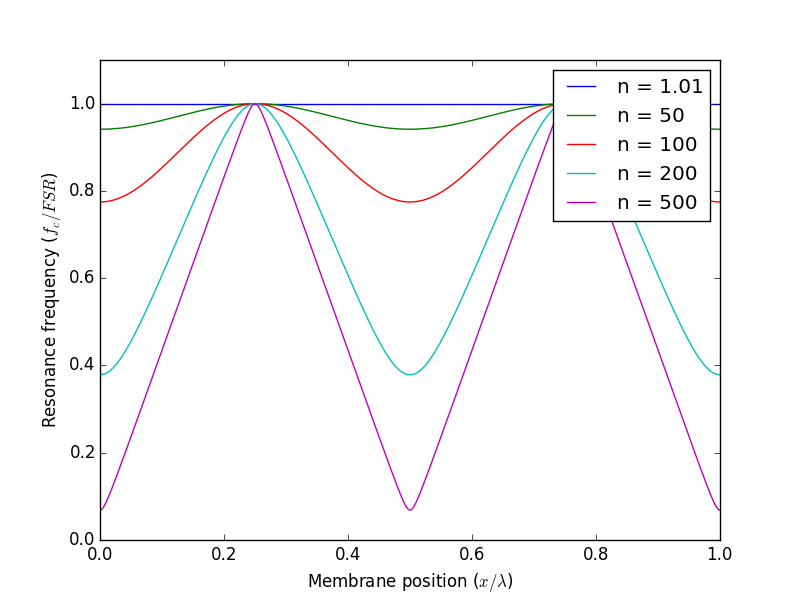
\includegraphics[scale=0.8]{transfer_matrix_python.png}
\caption{The membrane position is moved through one wavelength $\lambda$ with various reflection coefficients (index of refraction). The thickness is $d = 0.01$ \SI{}{\nano\meter} for the numerical simulation.}
\label{fig:transfer_model_plot}
\end{figure}

We previously introduced the optical frequency shift per displacement as $G = \frac{\partial\omega_c}{\partial x}$, i.e. the slope of the figure \ref{fig:transfer_model_plot}. It is an important parameter in our model, since our optically induced effects are quadratic in $G$. Clearly it must be advantageous to have the membrane placed at the steepest point on the slope. We also see that a membrane with fairly high reflectivity, gives a steeper slope and therefore also a higher coupling $G$. Another important message to take from this section is that the $FSR$ is no longer well defined.

\subsection{Hamiltonian formulation}
So far we have only described the optomechanical system classically and seen that it is absolutely possible to  among other things show cooling effects. It is now time to write out a full blown quantum mechanical model for our optomechanical system. We will start by writing out the Hamiltonian of a generic optomechanical system \cite{law1995}

\begin{equation}
\hat{H} = \hat{H}_{mech} + \hat{H}_{opt} + \hat{H}_{int} + \hat{H}_{drive}.
\end{equation}
\noindent
The full Hamiltonian consist of an optical drive $\hat{H}_{drive}$, an optical harmonic oscillator part for the cavity field $\hat{H}_{opt}$, a purely mechanical harmonic oscillator part $\hat{H}_{mech}$ (as equation \eqref{eq:ham_mech}) and most importantly the interaction part between mechanics and light $\hat{H}_{int}$. We write out the individual Hamiltonians

\begin{align}
\hat{H}_{mech} & = \frac{\hat{p}^2}{2m_{eff}} + \frac{1}{2}m_{eff}\Omega_m^2\hat{x}^2 \\
\hat{H}_{opt} & = \hbar\omega_c\left( \hat{a}^\dagger\hat{a} + \frac{1}{2}\right) \\
\hat{H}_{int} & = \hbar G\hat{x}\hat{a}^\dagger\hat{a} \\
\hat{H}_{drive} & = i\hbar\sqrt{\eta_c\kappa}(s_{in}(t)\hat{a}^\dagger - s_{in}^*(t)\hat{a}),
\end{align}
\noindent
where $\hat{x}$ and $\hat{p}$ are the position and momentum operators of the mechanical oscillator as in equation \eqref{eq:qm_pos} and \eqref{eq:qm_mom}, $m_{eff}$ is the effective mass and $\Omega_m$ is the angular mechanical resonance frequency. The operators $\hat{a}$ and $\hat{a}^\dagger$ are the annihilation and creation operators of the cavity mode and $\omega_c$ is the cavity resonance in angular frequency. $G$ is the optical frequency shift per displacement and $\eta_c = \frac{\kappa_{ex}}{\kappa_0 + \kappa_{ex}}$ is the coupling parameter for the cavity, where $\kappa_0$ is the intrinsic loss rate and $\kappa_{ex}$ is the external loss rate associated with the incoupling mirror, and $s_{in}(t)$ is the classical input drive field amplitude normalized to photon flux, previously we used $E_{in}(t)$ for this, but for easy comparison with the currently used notation in this group $s_{in}$ is used. The radiation pressure force is then 

\begin{equation}
\hat{F}_{rad} = -\frac{d\hat{H}_{int}}{d\hat{x}} = -\hbar G\hat{a}^\dagger\hat{a}.
\end{equation}

\subsection{Heisenberg-Langevin approach}
We want to obtain the quantum Heisenberg-Langevin equations \cite{gardiner2004} of the system. These equations are probably the most useful set of equations in this field of study. From them you can derive most physics optomechanical systems possess, at least for stuff like we do. We realize that the classical approach pressented in chapter \ref{sec:clas_opt_mech} is not far from the quantum picture, and is basically only missing an introduction of quantum vacuum fluctuations $\delta\hat{s}_{vac}(t)$. In the frame rotating at the laser frequency $\omega_l$ and with a detuning $\Delta = \omega_l - \omega_c$ we obtain the time evolution of the operators of interest \cite{schliesser2009, weis2010}

\begin{align}
\dot{\hat{a}}(t) & = \left( i\Delta - \frac{\kappa}{2} -iG\hat{x}(t) \right)\hat{a}(t) + \sqrt{\eta_c\kappa}\hat{s}_{in}(t) + \sqrt{(1 - \eta_c)\kappa}\delta\hat{s}_{vac}(t) \label{eq:h_lan1} \\
\dot{\hat{x}}(t) & = \frac{\hat{p}(t)}{m_{eff}} \label{eq:h_lan2} \\
\dot{\hat{p}}(t) & = -m_{eff}\Omega_m^2\hat{x}(t) - \hbar G\hat{a}^\dagger(t)\hat{a}(t) - \Gamma_m\hat{p}(t) + \delta\hat{F_{th}} \label{eq:h_lan3}
\end{align}
\noindent
where $\hat{s}_{in}(t) = \bar{s}_{in} + \delta\hat{s}_{in}(t)$ and $\bar{s}_{in}$ is a mean offset with a fluctuating noise perturbation $\delta\hat{s}_{in}(t)$. The noise terms in the system are $\delta\hat{s}_{in}$, $\delta\hat{s}_{vac}$ and $\delta\hat{F_{th}}$. The commutation relations and auto-correlations fulfill \cite{giovannetti2001}

\begin{align}
[\delta\hat{s}_{in}(t), \delta\hat{s}_{in}^\dagger(t')] & = [\delta\hat{s}_{vac}(t), \delta\hat{s}_{vac}^\dagger(t')] = \delta(t - t') \\
\langle \delta\hat{s}_{in}(t)\delta\hat{s}_{in}^\dagger(t') \rangle & = \langle \delta\hat{s}_{vac}(t)\delta\hat{s}_{vac}^\dagger(t') \rangle = \delta(t - t')
\end{align}
\noindent
We have here assumed zero thermal excitation of the optical mode, because optical frequencies are so high. Describing the correlation of the mechanical degree of freedom, which if undergoing Brownian motion has the autocorrelation \cite{gardiner2004}

\begin{equation}
\langle \delta\hat{F_{th}}(t)\delta\hat{F_{th}}(t') \rangle = \hbar m_{eff}\Gamma_m\int\frac{d\Omega}{2\pi} e^{-i\Omega(t - t')}\Omega\left( \coth\left( \frac{\hbar\Omega}{2k_bT} \right) + 1\right)
\end{equation}
\noindent
If we take the classical limit $\Omega\hbar \ll k_bT$ the equation above reduces to $\int\frac{d\Omega}{2\pi}m_{eff}\Gamma_mk_bTe^{-i\Omega(t - t')}$, which is similar to derived in equation \eqref{eq:thermal_drive}.

As shown in the classical picture we can simplify the equations of motion or in this case the quantum Heisenberg-Langevin equations of our system by considering the static and dynamical effects separately. We perform the unitary transformations $\hat{a}(t) = \bar{a} + \delta\hat{a}(t)$ and $\hat{x}(t) = \bar{x} + \delta\hat{x}(t)$, where the average of the fluctuating parts is zero $\langle \delta\hat{a}(t) \rangle = 0$ and $\langle \delta\hat{x}(t) \rangle = 0$. The static/steady state solution, i.e. $d/dt \rightarrow 0$, must fulfill

\begin{align}
\bar{a} & = \frac{\sqrt{\eta_c\kappa}\bar{s}_{in}}{-i(\Delta - G\bar{x}) + \frac{\kappa}{2}} \label{eq:ss_a} \\
\bar{x} & = \frac{-\hbar G \bar{a}^2}{m_{eff}\Omega_m^2}
\label{eq:ss_x}
\end{align}
\noindent
where $a$ is assumed to be real and positive. This system can give rise to a bistability for sufficiently strong drive fields \cite{weis2010, schliesser2009}. The bistability is a static classical effect. Letting $\hat{s}_{in}(t) = \bar{s}_{in} + \delta\hat{s}_{in}(t)$ and choosing the phase of the input field $\bar{s}_{in}$ such that $\bar{a}$ is real and positive, and assuming strong coherent drive ($1 \ll \bar{a}$), we get the linearized quantum Heisenberg-Langevin equations for the fluctuations. We again drop higher order terms like in the classical derivation. The linearized equations not surprisingly take the following form

\begin{align}
\delta\dot{\hat{a}}(t) & = \left( i\bar{\Delta} - \frac{\kappa}{2} \right)\delta\hat{a}(t) - iG\bar{a}\delta\hat{x}(t) + \sqrt{\eta_c\kappa}\delta\hat{s}_{in}(t) + \sqrt{(1 - \eta)\kappa}\delta\hat{s}_{vac}(t) \\
\delta\dot{\hat{a}}^\dagger(t) & = \left( -i\bar{\Delta} - \frac{\kappa}{2} \right)\delta\hat{a}^\dagger(t) + iG\bar{a}\delta\hat{x}(t) + \sqrt{\eta_c\kappa}\delta\hat{s}^\dagger_{in}(t) + \sqrt{(1 - \eta)\kappa}\delta\hat{s}^\dagger_{vac}(t),
\end{align}
\noindent
remember that $\bar{\Delta}$ is a new modified detuning, $\bar{\Delta} = \Delta -G\bar{x}$, see equation \eqref{eq:a_fluc}.

\begin{equation}
\delta\ddot{\hat{x}}(t) + \Gamma_m\delta\dot{\hat{x}}(t) + \Omega_m^2\delta\hat{x}(t) = \frac{1}{m_{eff}}\left( -\hbar G\bar{a}(\delta\hat{a}(t) + \delta\hat{a}^\dagger(t)) + \delta\hat{F}_{th}(t) \right)
\end{equation}
\noindent
We have used the property that $\delta\hat{x}(t) = \delta\hat{x}^\dagger(t)$. We solve these equations in the Fourier domain

\begin{align}
\delta\hat{a}(\Omega) & = \frac{-iG\bar{a}\delta\hat{x}(\Omega) + \sqrt{\eta_c\kappa}\delta\hat{s}_{in} + \sqrt{(1 - \eta_c)\kappa}\delta\hat{s}_{vac}(\Omega)}{-i(\bar{\Delta} + \Omega) + \frac{\kappa}{2}} \label{eq:da}\\
\delta\hat{a}^\dagger(\Omega) & = \frac{-iG\bar{a}\delta\hat{x}(\Omega) + \sqrt{\eta_c\kappa}\delta\hat{s}_{in}^\dagger + \sqrt{(1 - \eta_c)\kappa}\delta\hat{s}_{vac}^\dagger(\Omega)}{i(\bar{\Delta} - \Omega) + \frac{\kappa}{2}} \label{eq:dad} \\
\delta\hat{x}(\Omega) & = \frac{\left( -\hbar G\bar{a}(\delta\hat{a}(\Omega) + \delta\hat{a}^\dagger(\Omega)) + \delta\hat{F}_{th}(\Omega) \right)}{m_{eff}(\Omega_m^2 - \Omega^2 - i\Gamma_m\Omega)} \label{eq:dx}.
\end{align}
\noindent
The autocorrelation functions in frequency domain are

\begin{equation}
\langle \delta\hat{s}_{in}(\Omega)\delta\hat{s}_{in}^\dagger(\Omega') \rangle = \langle \delta\hat{s}_{vac}(\Omega)\delta\hat{s}_{vac}^\dagger(\Omega') \rangle = 2\pi\delta(\Omega - \Omega')
\end{equation}
\noindent
and

\begin{equation}
\langle \delta\hat{F_{th}}(\Omega)\delta\hat{F_{th}}(\Omega') \rangle = 2\pi\delta(\Omega - \Omega')\hbar m_{eff}\Gamma_m\Omega\left( \coth\left( \frac{\hbar\Omega}{2k_bT} \right) + 1\right),
\end{equation}
\noindent
these are the only non-zero correlators of the input noises.

\subsection{Limitation of dynamical backaction cooling}
As mentioned earlier in the classical picture section \ref{sec:clas_opt_mech}, we can supposedly cool the mechanical mode to  an arbitrary low phonon occupancy, if we neglect fluctuations of the input field and vacuum fluctuations. Introducing these fluctuations sets a theoretical lower bound to the phonon occupancy $n_{min}$ and thereby the amount of cooling one can achieve. We again write out the radiation pressure fluctuation in a similar manner as in the classical picture

\begin{equation}
\begin{split}
\delta\hat{F}_{rad}(\Omega) & = i\hbar G^2\bar{a}^2\left( \frac{1}{-i(\Delta + \Omega) + \frac{\kappa}{2}} - \frac{1}{i(\Delta - \Omega) + \frac{\kappa}{2}} \right)\delta\hat{x}(\Omega) \\ 
 & - \hbar G\bar{a}\frac{ \sqrt{\eta_c\kappa}\delta\hat{s}_{in} + \sqrt{(1 - \eta_c)\kappa}\delta\hat{s}_{vac}(\Omega)}{-i(\Delta + \Omega) + \frac{\kappa}{2}} \\
 & - \hbar G\bar{a}\frac{\sqrt{\eta_c\kappa}\delta\hat{s}_{in}^\dagger + \sqrt{(1 - \eta_c)\kappa}\delta\hat{s}_{vac}^\dagger(\Omega)}{i(\Delta - \Omega) + \frac{\kappa}{2}}.
\end{split}
\end{equation}
\noindent
The first line is the previously derived dynamical backaction driven by mechanical displacement, while the rest is known as quantum backacktion due to fluctuations of the intra-cavity photon number driven by fluctuation in the input drive and quantum vacuum fluctuations. We obtain the spectrum for the radiation pressure force caused by quantum backaction

\begin{equation}
S_{FF}^{qb}(\Omega) = \frac{\hbar^2}{2x_{zpf}}\left( A_- + A_+ \right),
\end{equation}
\noindent
where $A_{\pm}$ corresponds to the rates of anti-Stokes and Stokes scattering events in which phonons are annihilated or created

\begin{align}
A_- & = \frac{G^2\bar{a}^2x_{zpf}^2\kappa}{(\Delta + \Omega)^2 + \left(\frac{\kappa}{2}\right)^2} \\
A_+ & = \frac{G^2\bar{a}^2x_{zpf}^2\kappa}{(\Delta - \Omega)^2 + \left(\frac{\kappa}{2}\right)^2}.
\end{align}

We already know the classical contribution, so we actually only have to perform the integral, where dynamical backaction has been absorbed into $\chi_{eff}$

\begin{equation}
\langle\delta\hat{x}^2\rangle \propto \int\frac{d\Omega}{2\pi} \left| \chi_{eff}(\Omega)\right|^2S_{FF}^{qb}(\Omega) = \frac{A_- + A_+}{2\Gamma_{eff}}\hbar\Omega_m,
\end{equation}
\noindent
where $\langle\delta\hat{x}^2\rangle$ is equal to equation \eqref{eq:pos_fluc}, i.e. it contains a zero-point fluctuation term and $\Gamma_{eff} \propto \Gamma_{opt} \propto (A_- - A_+)$. Slightly different notation for $A_{\pm}$ was used in earlier chapters, but it can easily be rewritten to match this definition. A general cooling phonon number can be extrapolated to yield

\begin{equation}
\langle n\rangle \approx \frac{\Gamma_m}{\Gamma_{eff}}n_{bath} + n_{min},
\label{eq:nf}
\end{equation}
\noindent
where $n_{min} = \frac{A_+}{A_- - A_+}$ for significant cooling, i.e. $\Gamma_m \ll A_+ \ll A_-$. As a result of this added minimum phonon occupation number $n_{min}$ we can only reach the ground state $n < 1$ in the resolved sideband regime $\kappa \ll \Omega_m$, where it holds that

\begin{equation}
n_{min}^{res} \approx \left(\frac{\kappa}{4\Omega_m}\right)^2 \ll 1
\end{equation}
\noindent
In the unresolved regime $\Omega_m \ll \kappa $ the limit is $n_{min}^{unres} \approx \frac{\kappa}{4\Omega_m} \gg 1$.

\subsection{Optomechanical induced transparency}
We have now seen that radiation pressure coupling between an optical mode and a mechanical mode can lead to laser cooling of the mechanical mode if the control beam $\bar{s}_{in}$ is tuned to the red sideband transition of the optomechanical system. If we now also introduce a weak probe beam, this leads to destructive interference for the excitation of an intra-cavity probe field with the mechanical induced sideband field when $\omega_p = -\Omega_m$, thus inducing a transparency window for the probe beam oscillating at $\omega_p = \omega_l + \Omega$ \cite{weis2010}. Optomechanical induced transparency (OMIT) can be used to slow light, but we use it as an extremely useful tool to experimentally obtain otherwise hard-to-get parameters such as light-enhanced optomechanical coupling $g = Gx_{zpf}\sqrt{\bar{n}_{cav}}$ and detuning $\Delta$. We also get more accessible parameters as the cavity linewidth $\kappa$ and mechanical frequency $\Omega_m$.

We will start out by solving this problem for a drive field $s_{in}(t) = (\bar{s}_{in} + \delta s_{in}(t))e^{i\omega_l t}$, the perturbation term $\delta s_{in}(t) = s_pe^{-i(\omega_p - \omega_l)t}$ will later be identified with the probe field in the linearized Heisenberg-Langevin equations. We assume that all the drives are weak classical coherent fields, resulting in all expectation values of operators will replaced with the classical term, e.g. $\langle\delta\hat{a}(t)\rangle \equiv \delta a(t)$. All quantum and thermal noise terms average to zero. We solve the coupled linearized equations of motion \eqref{eq:da}, \eqref{eq:dad} and \eqref{eq:dx} for the intra-cavity field $(\bar{a}^\dagger(\Omega)\delta\hat{a}(\Omega) + \bar{a}(\Omega)\delta\hat{a}^\dagger(\Omega))$. The analytic expression is to cumbersome to be shown here and obtain the solution using Mathematica. A theoretical prediction of the model is shown in figure \ref{fig:omit_theory_lol}.

\begin{figure}[H]
\centering
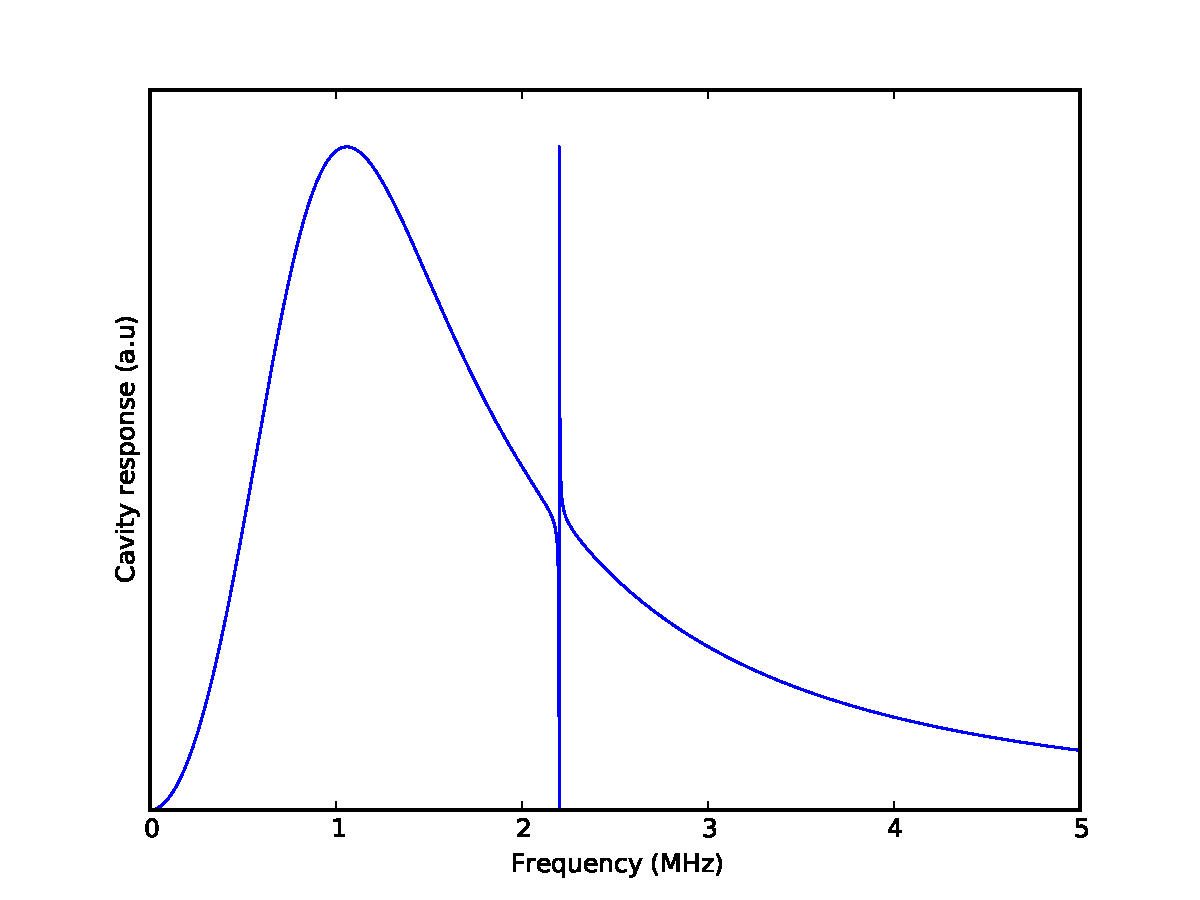
\includegraphics[scale=0.7]{omit_theory.pdf}
\caption{Theoretical prediction of the OMIT model, for $\kappa/2\pi = $ \SI{1.5}{\mega\hertz}, $\bar{\Delta} = -\kappa/2$, $\Omega_m/2\pi = 2.2$ \SI{}{\mega\hertz} and $g/2\pi = 100$ \SI{}{\kilo\hertz} .}
\label{fig:omit_theory_lol}
\end{figure}

\chapter{Experimental setups and procedures}

\section{Optical setup}
The purpose of this section is to give a detailed schematic of our optical table setup. The setup is divided into two parts, a pre-setup part describing how we manipulate the cavity input and lock the laser to the cavity and a second part including the cavity and detection scheme. It should be noted that three persons have simultaneously been working on the setup, so the setup is constantly being altered to fit the current workloads. We begin with the pre-setup shown in figure \ref{fig:presetup}.

\begin{figure}[H]
\centering
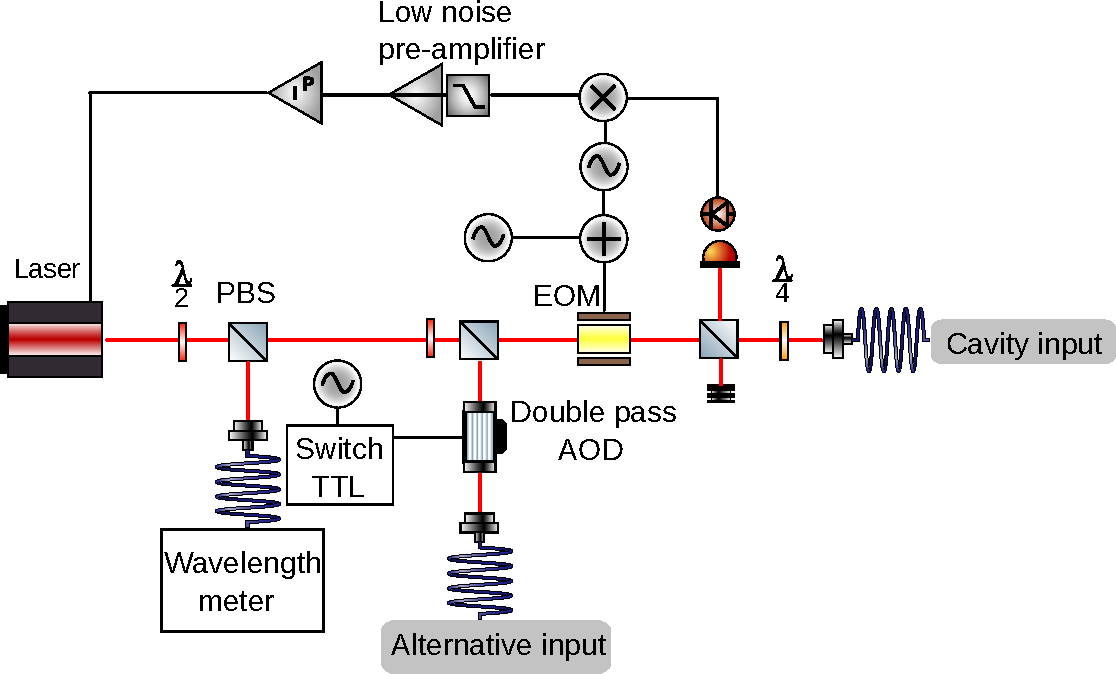
\includegraphics[scale=0.8]{setup.pdf}
\caption{Detailed overview of the pre-setup on our optical table.}
\label{fig:presetup}
\end{figure}

\subsection{Input}
The laser used is a narrow linewidth widely tunable CW titanium sapphire (Ti:sapphire)\footnote{MSquared SolsTiS}. It has the special property of having a low phase noise and a low relative intensity noise for the frequencies we want to work at, meaning that we are shot noise limited at roughly \SI{1}{\mega\hertz} and upwards (see appendix \ref{sec:rin}). The laser comes with commercial control software for tuning/scanning the wavelength and locking it to its external reference cavity for stability. It can be operated with a wavelength in the range 725-975 \SI{}{\nano\meter} and it has a narrow linewidth of \SI{18}{\kilo\hertz} if locked to its reference cavity.

The laser light enters the pre-setup and is directly split into two beams by a half wave plate ($\lambda/2$) and polarizing beam splitter (PBS). Most of the optical power is transmitted through the PBS. The reflected beam is fiber coupled and sent to a Bristol 521-NIR wavelength meter which has an accuracy of \SI{\pm 10}{pm}, since the built-in commercial wavelength meter in the laser is not accurate enough $\pm 100$ pm. The Bristol wavelength meter is then connected to a computer, where we read off the wavelength.

\subsection{Primary input}
The transmitted beam after the first PBS is split again by a $\lambda/2$-plate and a PBS. The transmitted beam is sent to a fiber coupled \SI{10}{\giga\hertz} electro-optical-modulator\footnote{EOSpace PM-0K1-10-PFU-PFU-850-UL-S} (EOM), which takes two inputs from signal generators to generate a sideband for the locking scheme as wel as one for sweeping a probe field across the cavity resonance. The output from the EOM is sent through a PBS and a quarter wave plate ($\lambda/4$) and then fiber coupled and sent as primary input to the cavity. The $\lambda/4$-plate and PBS is in reality a three armed fiber coupled beam splitter, which sends the cavity reflection to a fiber coupled photodetector\footnote{Thorlabs PDA8GS}. For illustrative reasons it is pictured as a wave plate and a PBS. The detector in reflection is used to both set up a Pound-Drever-Hall lock \cite{black2001}, and as a tool for optimizing backreflection from the flat bottom mirror during the assembly procedure. For the lock feedback we use a low noise pre-amplifier\footnote{Stanford Research Systems SR560} and a commercial servo box\footnote{New Focus LB1005 Servo Controller}. We do not use the PDH lock for the experiments presented here, so the error signal is then taken from the transmission detector.

\subsection{Alternative input}
The reflected beam of the PBS in the middle is sent to a double-pass \SI{120}{\mega\hertz} acuosto-optic deflector\footnote{IntraAction corp. ATD-1202DA2} (AOD) setup, such that we can modulate without misaligning the beam path. The AOD is driven by a signal generator connected to a home-built TTL switch board. This alternative input serves the purpose of optically exciting the membrane's mechanical modes, as will be explained in detail in section \ref{sec:q_fact}.

\subsection{Cryo-cavity and detection}
In the lab lingo, we often refer to our setup as the cryo-cavity setup and now the name has also found its way into this work. See figure \ref{fig:cryocavity} for a detailed overview. The fiber from pre-setup is attached on a fiber output-coupler, where tilt/angle can be adjusted. The output-coupler is placed on a XYZ-stage. These degrees of freedom are crucial for alignment of the cavity, fixing membrane mirror tilt and optimizing optomechanical coupling. Right after the the coupler a lens ($f = $\SI{11}{\milli\meter}) is placed to mode match the wave fronts to the cavity. The transmission from the cavity is then put on a 92:8 beamsplitter, where the reflected beam is sent to a camera\footnote{Mightex} and the transmitted beam is put on a photodetector\footnote{Thorlabs APD110A}. The detector signal is split into a DC part and RF part by a Bias Tee\footnote{Mini Circuit ZF8T-4R2G} with a cuf-off frequency of \SI{10}{\mega\hertz}. The DC part of the signal is then sent to an oscilloscope and RF part is sent to a network analyzer or sometimes just a spectrum analyzer depending on the situation. For the work presented in here we setup the lock using the transmission detector for a simple slope lock, which will be described in section \ref{sec:exp_omit}.

\begin{figure}[H]
\centering
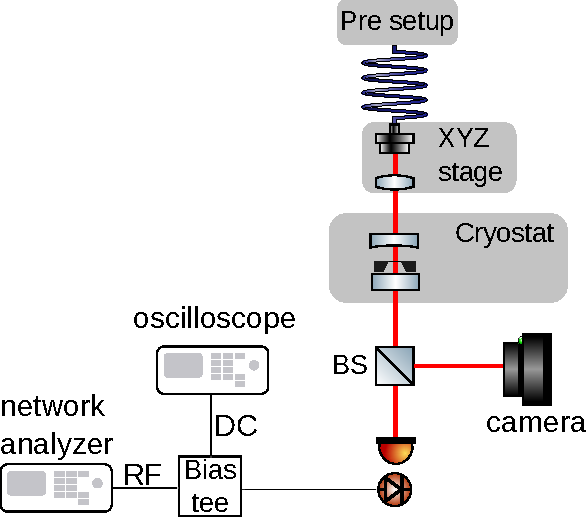
\includegraphics[scale=1.1]{cryocavity.pdf}
\caption{Cryo-cavity setup.}
\label{fig:cryocavity}
\end{figure}

\section{Mirrors}
Since no mirror specification was available for our super mirrors, we decided to obtain our own experimentally, see figure \ref{fig:trans_mirrors}. We expected, at optimal wavelength \SI{852}{\nano\meter}, to get very tiny transmissions on order tens of part per million (ppm). Therefore normal means did not work, i.e. just measuring power before and after the mirror with a power meter. To obtain the data we used the tunable Ti:Sapph laser, the output of which was sent through an AOD connected to the TTL switch board, such that the light was fully amplitude modulated at an arbitrary frequency. A detector was placed after the mirror and its output was sent to a lock-in amplifier and demodulated at the given amplitude modulation frequency. The resulting mirror transmissions as function of wavelength are shown in figure \ref{fig:trans_mirrors}.

\begin{figure}[H]
\centering
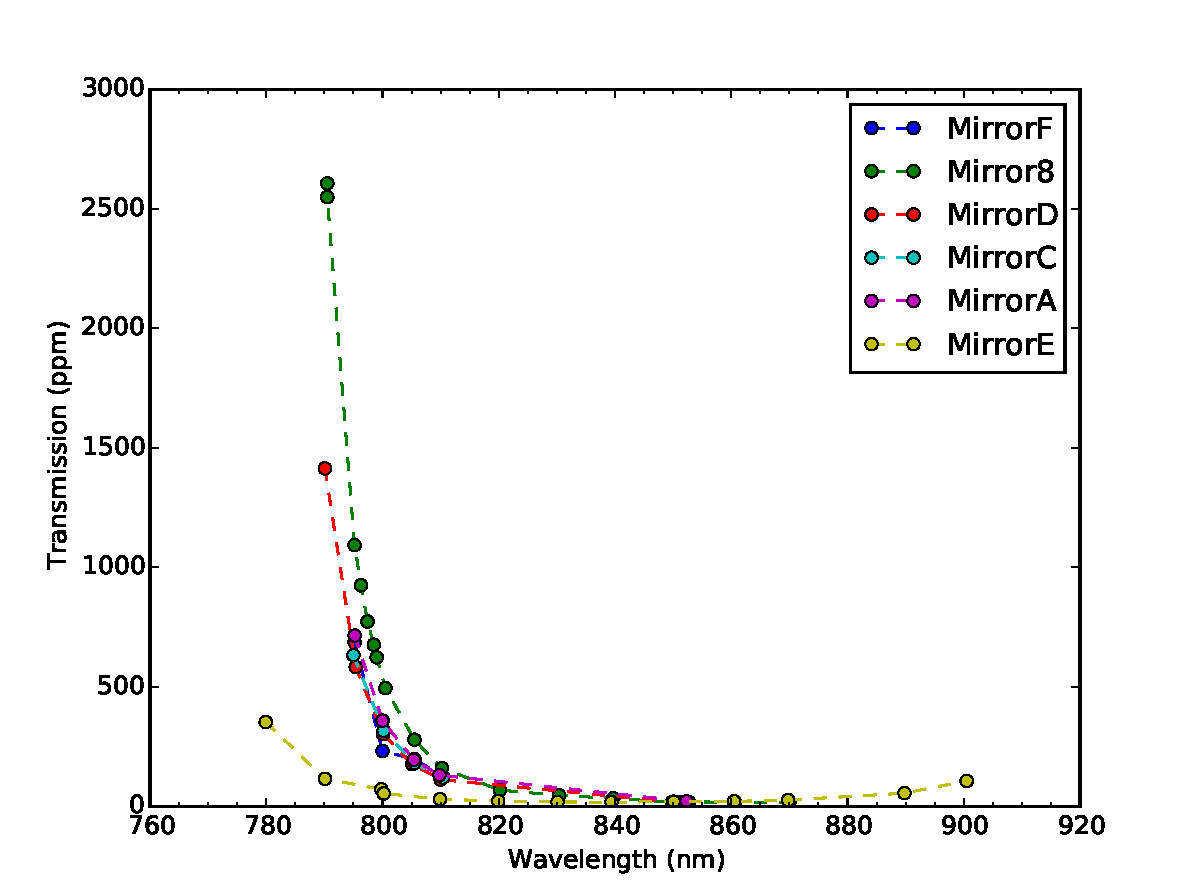
\includegraphics[scale=0.7]{mirror_transmissions.pdf}
\caption{Transmission as a function of wavelength for our super polished mirrors. They all have the same transmission curve except from the ``special" mirror 8, which has a curve shifted of the rest. Mirrors denoted with a letter are curved and mirrors with a number are flat.}
\label{fig:trans_mirrors}
\end{figure}

Simultaneously we were testing mirrors with different coatings, to find a curved mirror with a higher transmission than the flat bottom mirror, in order to utilize a different cavity coupling regime instead of a critical coupled one, see section \ref{sec:opt_cav}. Whereas critical coupling is good for cooling, different experiments, such as squeezing, call for an alternative coupling regime. By coincidence we found that one of our already in stock super mirrors had a slightly shifted transmission curve, clearly deviating from the rest of the mirrors from the same coating run. Mirror 8 combined with mirror E has the most shifted apart transmission curves, but still fulfill critical coupling with each mirror presenting \SI{20}{ppm} at \SI{852}{\nano\meter} see figure \ref{fig:trans_e_8}.


\begin{figure}[H]
\centering
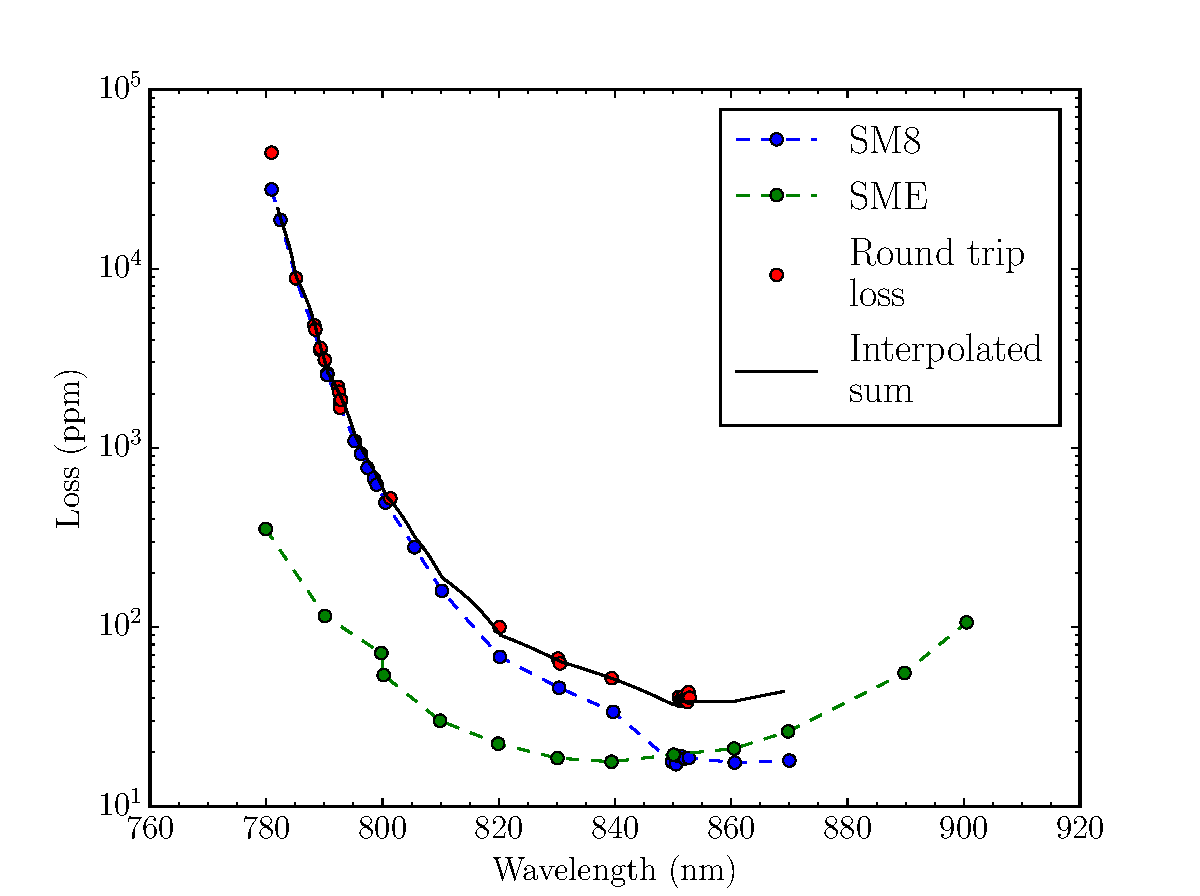
\includegraphics[scale=0.7]{mirror_e_8.pdf}
\caption{Mirror transmission presented on a log scale for mirrors 8 (green) and E (blue). An interpolated sum (black) of the two mirror transmissions together with an actual measured round trip loss (red) for an assembled bare cavity shows that these two mirrors have very little loss, when combined into a cavity.}
\label{fig:trans_e_8}
\end{figure}

By tuning our wavelength up or down in wavelength, we can choose how deep into the different cavity coupling regimes we can be. This is truly a neat feature of our cavity.

\section{Bare cavity characterization}
First task of utilizing a membrane-in-the-middle system, for doing cavity optomechanics, is to build a cavity and measure its properties before complicating things, by putting a membrane inside it. Our Fabry-Perot cavity (in all its simplicity), consists of a flat bottom mirror and a curved top mirror, which is the in-coupling mirror. This is a stable configuration if the radius of curvature of the curved mirror is larger than the cavity length $R > L$, which is satisfied in our case since $R = 2.5$ \SI{}{\centi\meter} and the cavity length is $L \sim 1.5$ \SI{}{\milli\meter}. The waist of the beam (radius) $w_0 \sim$ \SI{40}{\micro\meter} is placed at the flat mirror by a movable lens of focal length $f = 11$ \SI{}{\milli\meter}. For a desired distance to the bottom mirror, this condition mode matches the wavefront curvature to the mirrors curvature at wavelength $\lambda = 850$ \SI{}{\nano\meter} according to basic Gaussian optics see figure \ref{fig:bare_cavity}. The free spectral range of the cavity is $100$ \SI{}{\giga\hertz}. The rather short cavity length is chosen to increase the coupling $G = \frac{\omega_c}{L}$ as much as possible. The spot size $w_0$ is another important parameter, since we want to resolve the membrane mode shapes $\frac{L_m}{n} > w_0$, where $L_m$ is the side length of the membrane and $n$ is the highest mode number. Not being deeply in this regime results in a decreased coupling, because of the overlap integral between mechanical mode and spot size.

\begin{figure}[h]
\centering
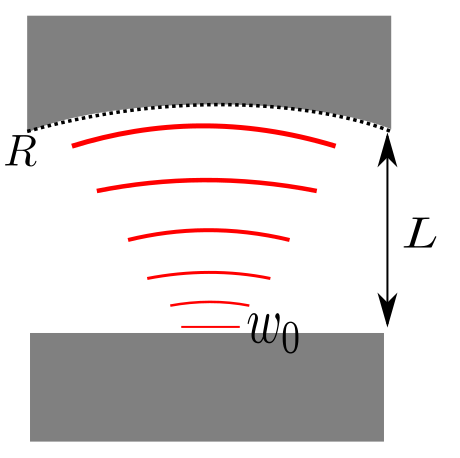
\includegraphics[scale=0.5]{cavity.png}
\caption{Bare cavity design.}
\label{fig:bare_cavity}
\end{figure}

We measure our bare cavity linewidth at \SI{852}{\nano\meter} to be roughly \SI{0.5}{\mega\hertz} as shown from the trace in figure \ref{fig:bare_cavity_linewidth}\footnote{$\kappa$ in the figure is actually $\kappa/2\pi$}. The axis is calibrated using EOM generated sidebands at \SI{3}{\mega\hertz} and the cavity linewidth $\kappa/2\pi$ is obtained by a Lorentzian fit.

\begin{figure}[h]
\centering
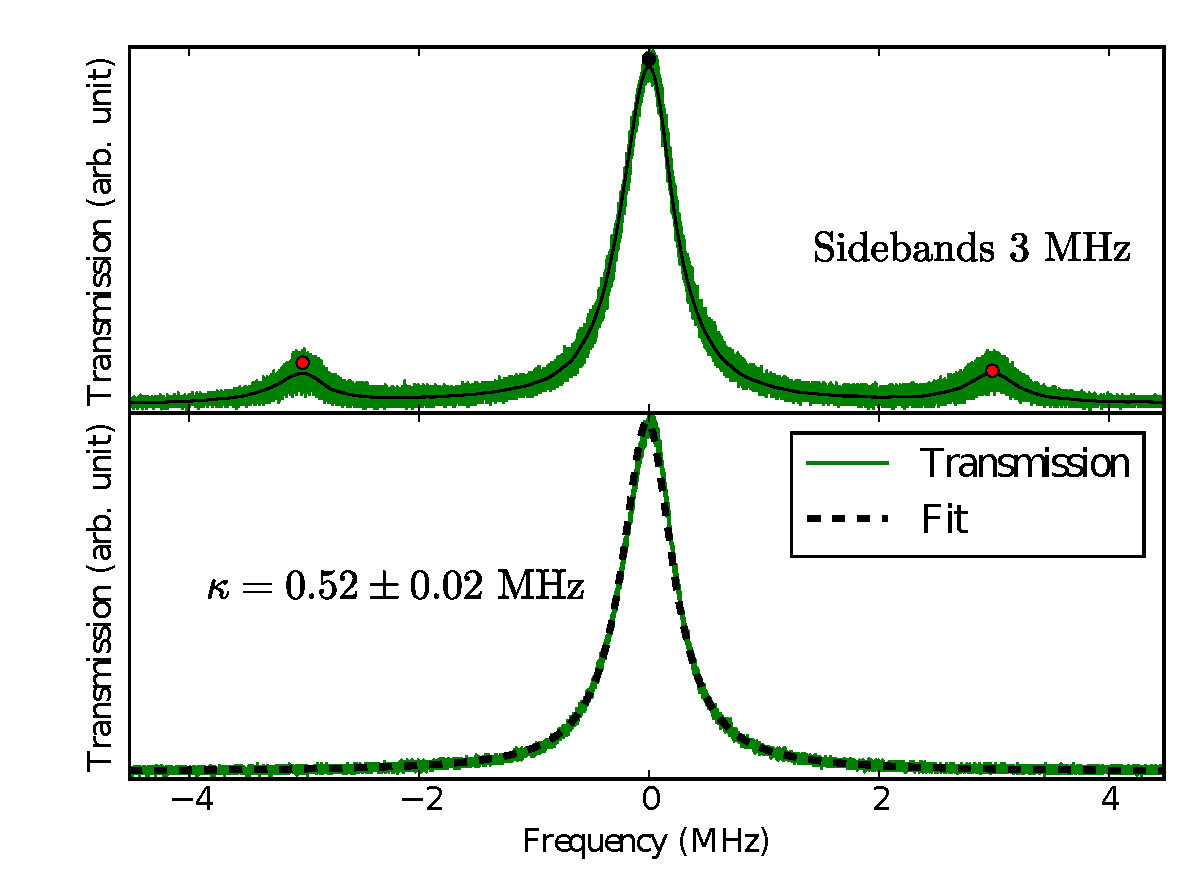
\includegraphics[scale=0.7]{cavity_linewidth.pdf}
\caption{Bare cavity linewidth measured by calibrating the frequency axis using sidebands.}
\label{fig:bare_cavity_linewidth}
\end{figure}

The bare cavity free spectral range is measured to be \SI{84.9}{\giga\hertz} see appendix \ref{sec:bare_fsr}. The assembled bare cavity is a bit longer than initially intended, but the added length can be assigned to the curvature of one of the mirrors. Our measured cavity finesse is then roughly 163000, which is a high finesse for optical cavities.

\section{Sample}
Prior to using a one-dimensional phononic bandgap on our high-stress silicon nitride (\ce{Si3N4}) membrane sample, we used commercial fabricated Norcada \ce{Si3N4} membranes\footnote{\url{http://www.norcada.com/products/high-q-si3n4-membrane/}}. However, they suffered greatly from reduction of quality factor $Q$ when clamped \cite{wilson2009}. The overall goal is to have a quantum enabled system and that means for most experiments, i.e. squeezing \cite{purdy2013} and ground state cooling \cite{chan2011}, cryogenically pre-cooling the membrane as much as possible, before starting the experiments. This is due to the fact that our final phonon occupancy is proportional to the bath temperature as shown in equation \eqref{eq:nf}. This requires clamping of the sample to achieve good thermal flow from the cold finger to the sampler holder and into the sample. At the same time we do not want to compromise the $Q$'s in order to do so. Luckily the idea of membrane shielding by a phononic bandgap was proposed \cite{tsaturyan2014, yu2014} and fabricating them is a huge step in the right direction for the membrane-in-middle optomechanical system. A picture of such a membrane is shown in figure \ref{fig:sample}. For insight into fabrication processes see \cite{tsaturyan2014}.

\begin{figure}[H]
\centering
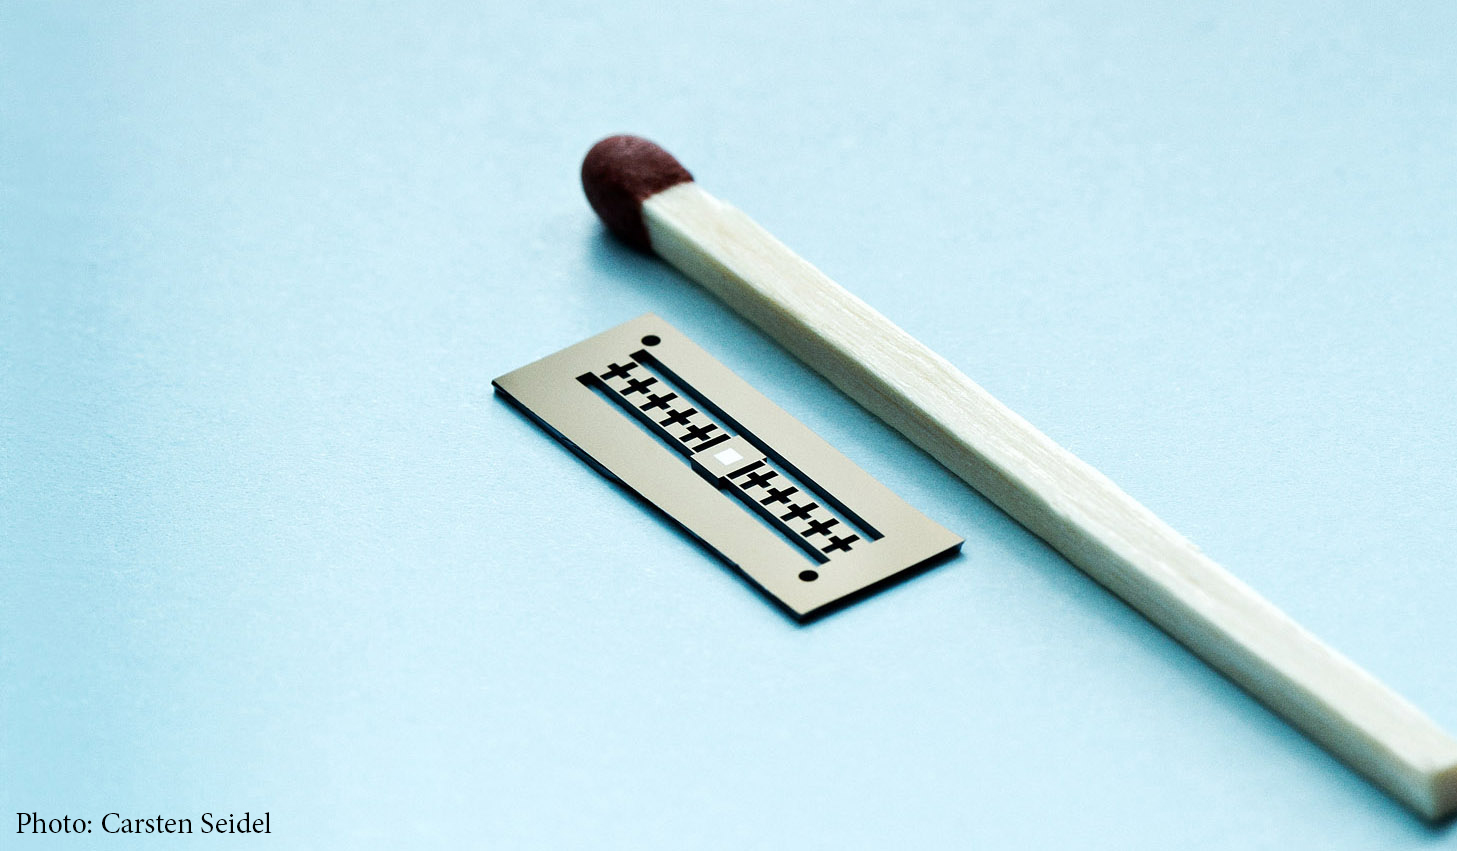
\includegraphics[scale=0.25]{Seidel_02.jpg}
\caption{Silicon nitride membrane shielded by a one-dimensional phononic bandgap next to a match for size comparison.}
\label{fig:sample}
\end{figure}

A problem with this generation of samples, is the low fundamental frequency ($\sim$\SI{13}{\kilo\hertz})\cite{tsaturyan2014} of the phononic bridge, on which the membrane is suspended on. Due to the low frequency of the bridge mode, there is significant excitaions from the surrounding environment. This makes locking the laser to the cavity resonance with high input powers very challenging. Therefore, in this work we were forced to dampen the bridge by placing chips with no suspended membranes on both sides of the actual test sample, thus disabling the effect of the phononic shield.

As a small side remark we also make spacers for the cavity assembly, which is done breaking of the phononic bridge of a normal chip. Since the surface of the silicon is extremely smooth, they make a good spacer, as will be evident in the section below.

\section{Sample holder}
The motivation for making a new sample holder was that we got new samples that no longer fit in the old one. The other reason was that the old sample holder did not thermalize the sample very well. Good thermalization of the sample is of high priority. With the new samples came the opportunity to clamp the frame of our sample without notable reduction of mechanical $Q$, as shown \cite{tsaturyan2014}.

A lot of good ideas and considerations sprung from the process of designing a new sample holder. Here is a list of the most noticeable:

\begin{itemize}
\item The sample holder build material should be oxygen-free high thermal conductivity (OFHC) copper, for best thermal conductivity properties at cryogenic temperatures.
\item Minimize the number of sample holder parts between sample and cold finger, as each transition adds a barrier in thermal flow.
\item Minimize the angle of incidence, to shield from thermal radiation.
\item Placing a spacer-membrane-spacer stack on the flat bottom mirror as possible: a) to avoid tilt between flat mirror and membrane and thereby achieve good parallelism, any tilt will induce extra loss. b) to have a smaller mismatch between the wave fronts of the cavity field with the membrane, since we have nearly planar waves at the beam waist placed on the flat bottom mirror, and therefore less scattering loss.
\item Use springs to push the mirrors hard against the spacer-membrane-spacer stack, which again is to achieve parallelism and to have a vibration stable cavity while operating at cryogenic temperatures.
\item Have as large as possible clamping area between sample and sample holder, for good thermal flow.
\end{itemize}

The assembled sample holder containing springs, a cavity and a membrane stack is shown in figure \ref{fig:sample_holder_tilt}.

\begin{figure}[H]
\centering
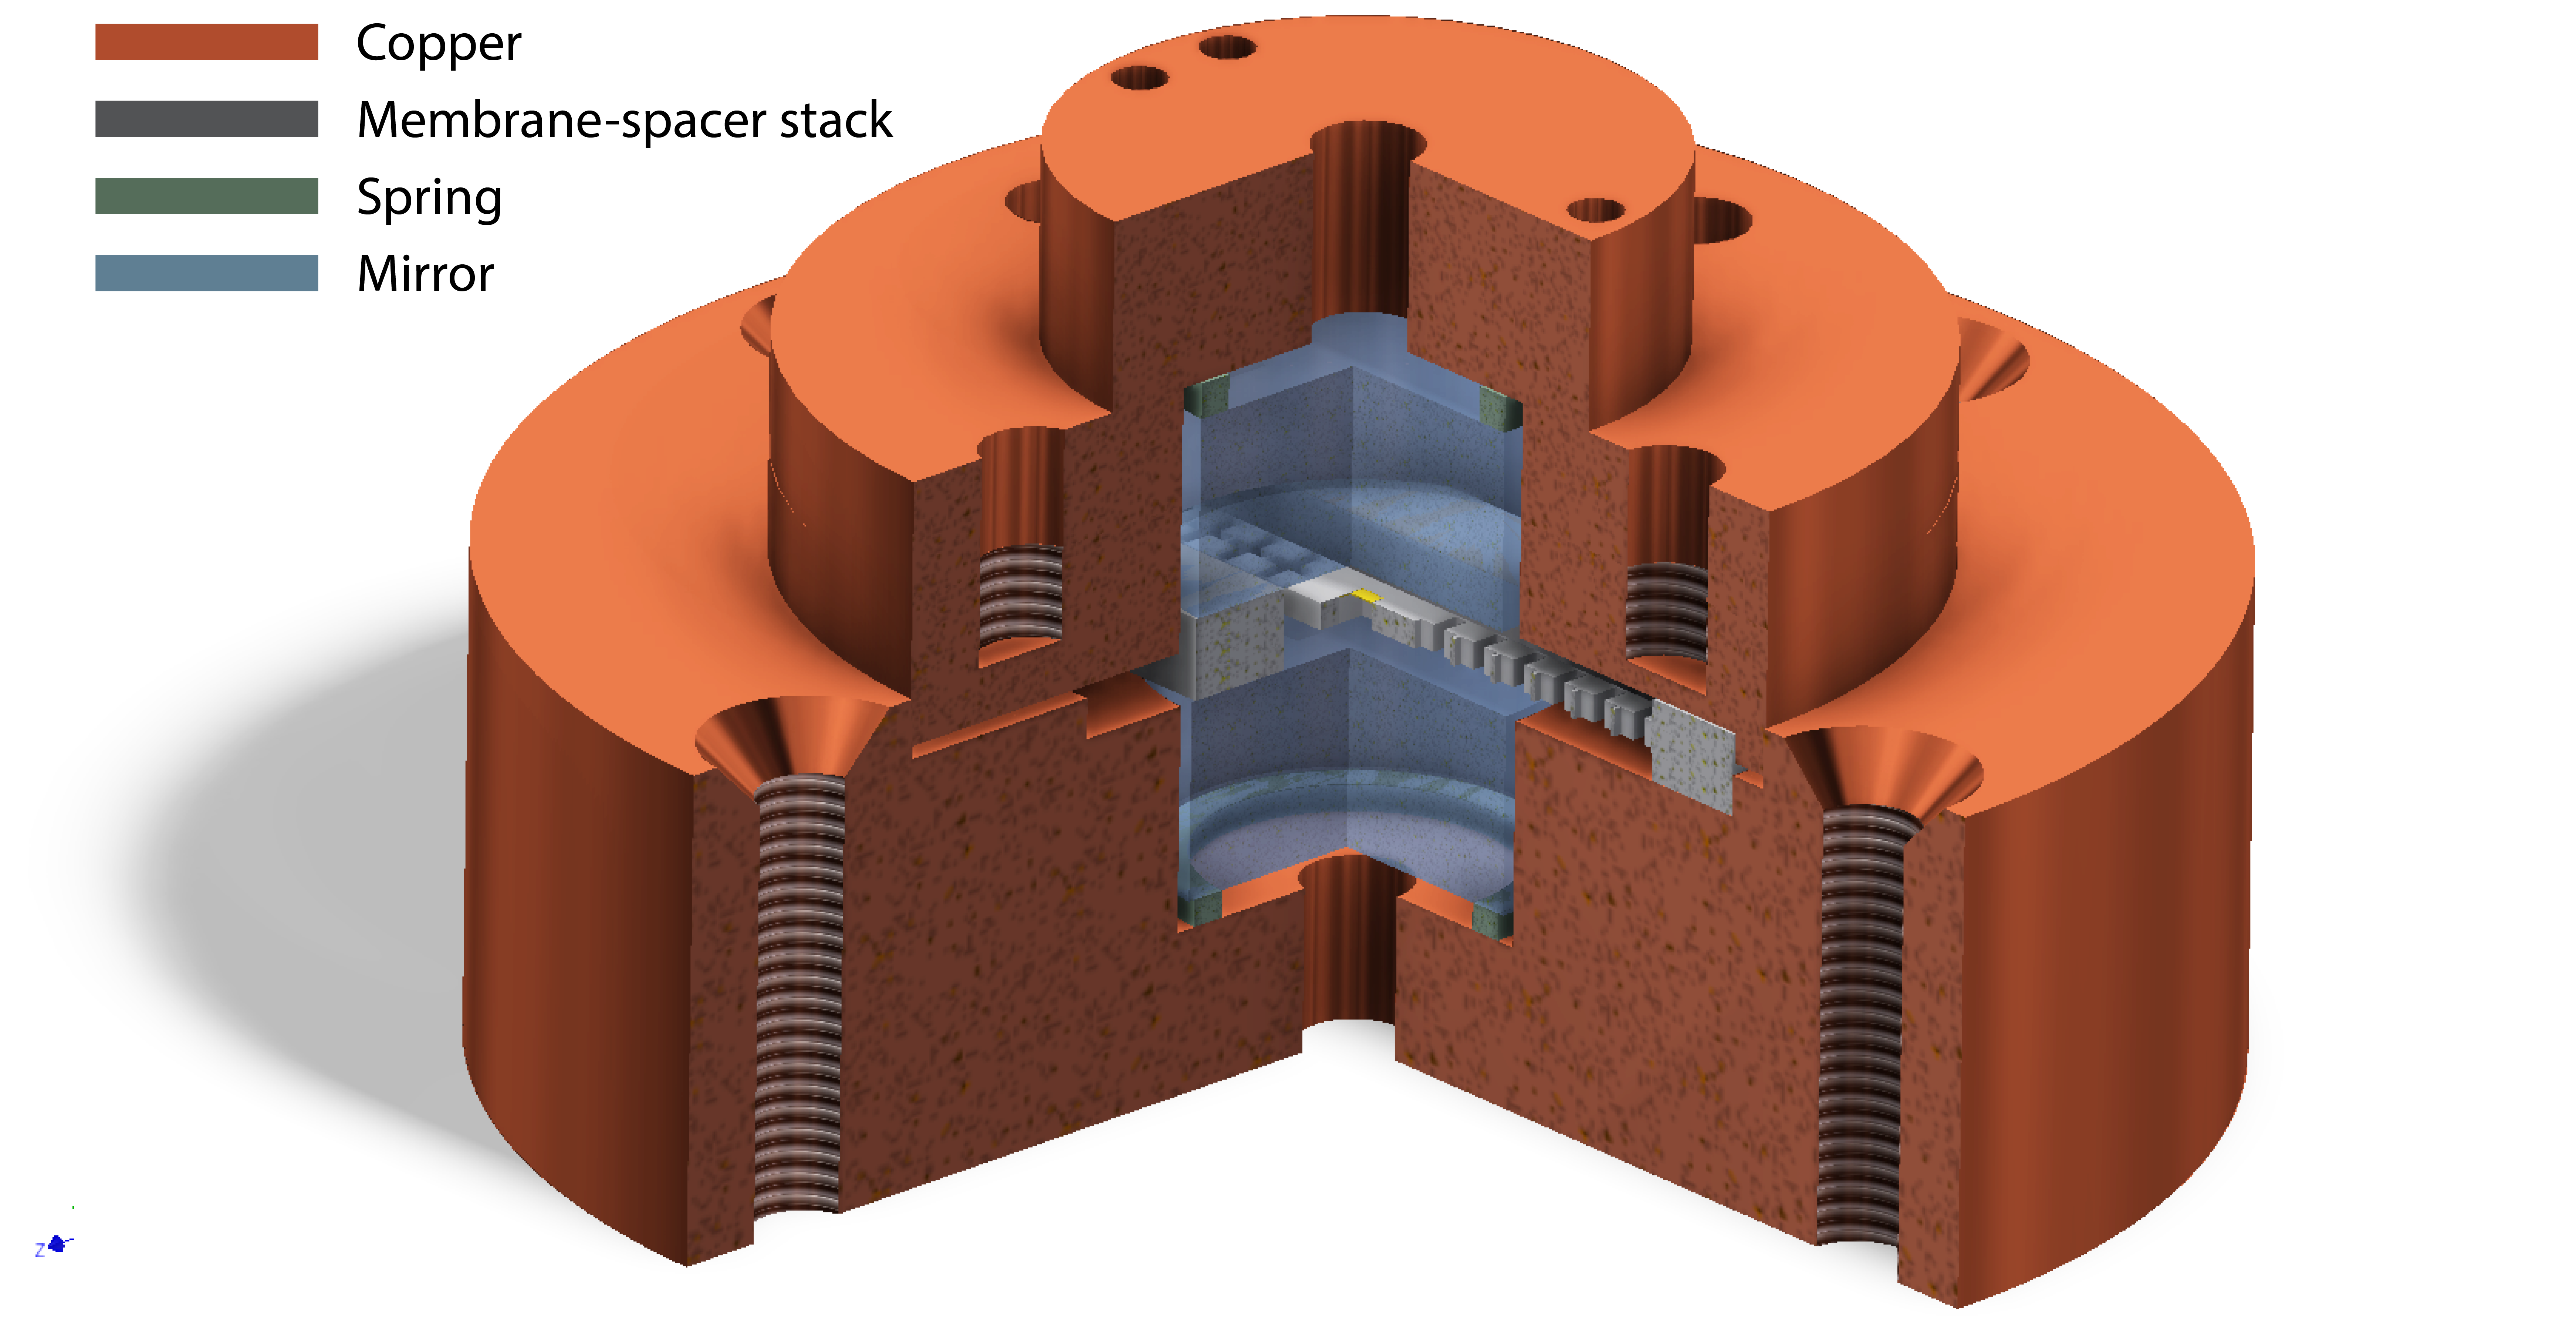
\includegraphics[scale=0.2]{bigBud_v09_new.png}
\caption{Fully assembled sample holder.}
\label{fig:sample_holder_tilt}
\end{figure}

Let us describe the sample holder's three parts piece by piece, starting with the bottom part. It is \SI{30}{\milli\meter} in diameter and has four threaded holes, matching holes in the cold finger, such that it can be firmly anchored in the cold finger of the cryostat and act as good thermal bridge to the rest of the sample holder. A small hole going all the way through with \SI{2}{\milli\meter} in diameter is placed in the middle, allowing for light to pass through, but with a small enough angle of incident, so as to limit thermal radiation. The hole for the spring and flat bottom mirror are machined to have the quarter inch mirror sticking a bit out of the hole (dependent on choice of spring), such that the membrane stack can compress the spring and enable parallelism between mirror and membrane surface. A small groove to fit the membrane stack is made to account for alignment of the membrane, but since the couple first generation of membranes chips did not have well defined edge dimensions, the size of the groove's length dimensions was extended to accommodate for this uncertainty and in the end made alignment more difficult. Four threaded holes for the middle part to fasten and a little groove for the middle part to fit in is cut. The middle part can be hard to separate from the top part in figure \ref{fig:sample_holder_tilt}, for more details see figure \ref{fig:sample_holder_pull}, where the sample holder parts are pulled apart. The middle part is a disk \SI{20}{\milli\meter} in diameter. On the side facing towards the bottom part there is also a small grove like the one in the bottom part to align the membrane stack. The middle part pushes the membrane stack and compresses the bottom spring when screwed into the bottom part. The membrane stack then gets thermalized through the middle piece. A hole is machined in the middle where the top curved mirror is placed. The four tiny holes in pairs of two is to allow air to escape upon evacuation of the cryostat. The top part can be fastened to the middle part. It looks like a hat and it is in fact hollow, such that it can glide down on the top mirror with a spring placed on top. There is a small \SI{2}{\milli\meter} hole for incoupling in the top part as well.

\begin{figure}[H]
\centering
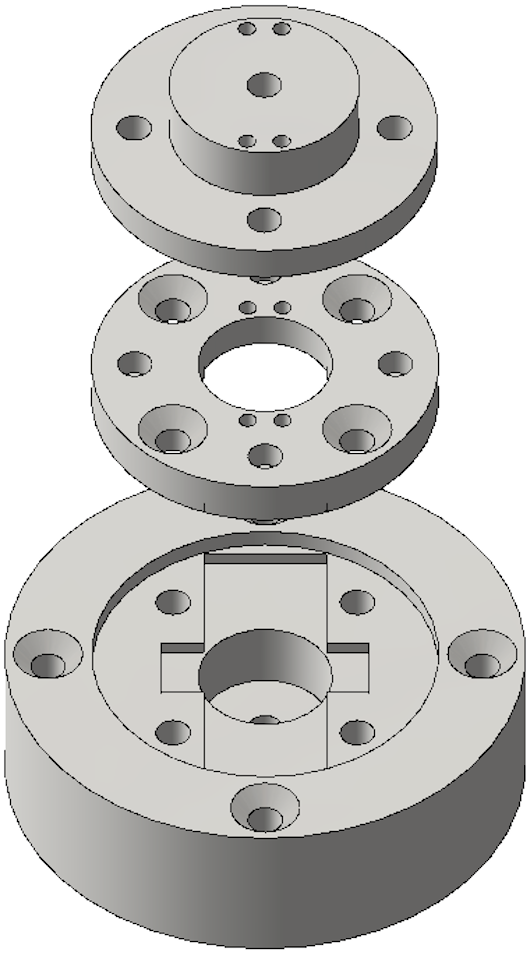
\includegraphics[scale=0.5]{side_topv2.png}
\caption{Sample holder pulled apart. The color scheme is changed to grey scale for better detail outline.}
\label{fig:sample_holder_pull}
\end{figure}

The sample chips have a height of \SI{0.5}{\milli\meter}, and thus the spacer-membrane-spacer stack is roughly the cavity length of $L \approx 1.5$ \SI{}{\milli\meter}. As springs we use thin copper washers custom bent in three places to form a wave spring. See figure \ref{fig:sample_holder_inside} for assembly inside the sample holder.

\begin{figure}[H]
\centering
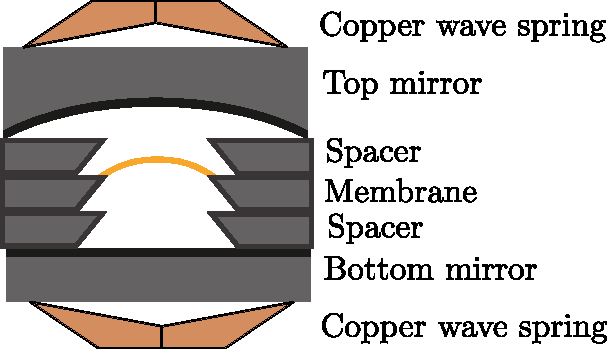
\includegraphics[scale=0.7]{mim_setup.pdf}
\caption{Assembly inside the sample holder.}
\label{fig:sample_holder_inside}
\end{figure}

A thing that we did not anticipate, was that we would need to push around the top mirror horizontally to finally align the cavity. The hope was that the geometry of the sample holder solved this problem, but sadly it did not. To enable this degree of freedom, we drilled four small opposite holes in sides of the top part of the sample holder, allowing for small metal rods to push the top mirror around. We called it the ``pinhead" solution. It was somewhat cumbersome, but it got the job done.

By a communication error we ended up having the sample holder made in the material Elmedur, which is another alloy of copper instead of oxygen-free copper. This mistake was first realized after the data was taken.

\section{MIM assembly procedure}
This section serves as a detailed description of how we fully assemble the membrane-in-the-middle setup. It is a long and sometimes tedious procedure. Most of the procedure is constructed from educated guesses, while a procedure like fixing the membrane versus flat mirror tilt is pure luck, i.e. trial and error.

\subsection{Cleaning}
To achieve good vacuum the sample holder including screws, springs and membrane spacers is cleaned in high purity acetone inside an ultra-sonic bath for roughly 20 minutes. After the ultra-sonic bath the parts are pulled out of the acetone, in as clean conditions as possible inside a lab/fume hood, and cleaned with ``ultrapure\footnote{Millipore}" water to get rid of any residual acetone and small impurities. The parts are then put aside to dry on the inside of a piece of aluminum foil. When dried the parts are ready to used inside our cryostat.

We depend a lot on our mirrors to have low losses and they fulfill this task. But mirrors can also become dusty or dirty from small broken silicon parts of the spacers. The tiny silicon impurities on the mirrors can occur when tightening the screws between middle and bottom part of the sample holder because it sometimes happens that the membrane stack is slightly misplaced and silicon pieces are broken of the stack. We clean the mirrors with a polymer\footnote{First Contact. Nice videos showing this procedure can be found on \url{https://www.youtube.com/watch?v=YWp8k8s8aeM}.} evenly distributed on the coated mirror surface. The polymer dries out and can be pulled of with a suitable adhesive tape. The mirrors are then checked under a microscope before being put into use.

It is important to use and wear for example clean plastic tweezers, rubber gloves, hairnet and face mask, while cleaning the individual parts for minimizing contamination as much as possible.

\subsection{Back reflection}
We tightly screw the bottom sample holder piece into the cold finger inside the cryostat, and place a copper wave spring with the flat mirror on top of it inside the hole in the sample holder. The flat mirror is now resting on the spring. We then shine laser light on to the mirror and try to maximize back reflection through the fiber. Backreflection coupled in to the fiber is maximum, when you mode-match, i.e have the waist on the flat mirror. It allows for a good initial parameter for mode matching.

\subsection{Membrane tilt}
The next step is to carefully assemble the spacer-membrane-spacer stack and place it on top of the flat mirror. The middle sampler holder part is put onto the stack and screwed into place compressing the spring and making a tight and hopefully parallel fit between membrane surface and mirror surface. The membrane and the mirror now make up an unstable low finesse cavity, due to the relative low reflectivity coefficient of the silicon nitride membrane. It is this cavity that enables us via scanning the fiber output coupler in the same plane as the combined membrane-mirror plane to observe cavity resonance fringes. The tilt angle can be extrapolated from number of fringes showing up on the oscilloscope. Each fringe corresponds to another half wavelength fitting into the cavity and if we note down the range of the scan we also know the angle from simple geometry. The goal is to eliminate fringes by trial and error, by pushing unscrewing the middle piece a little bit and then screwing it back in again. A successful attempt is shown in figure \ref{fig:mem_tilt}.

\begin{figure}[H]
\centering
    \begin{subfigure}[b]{0.49\textwidth}
    \centering
    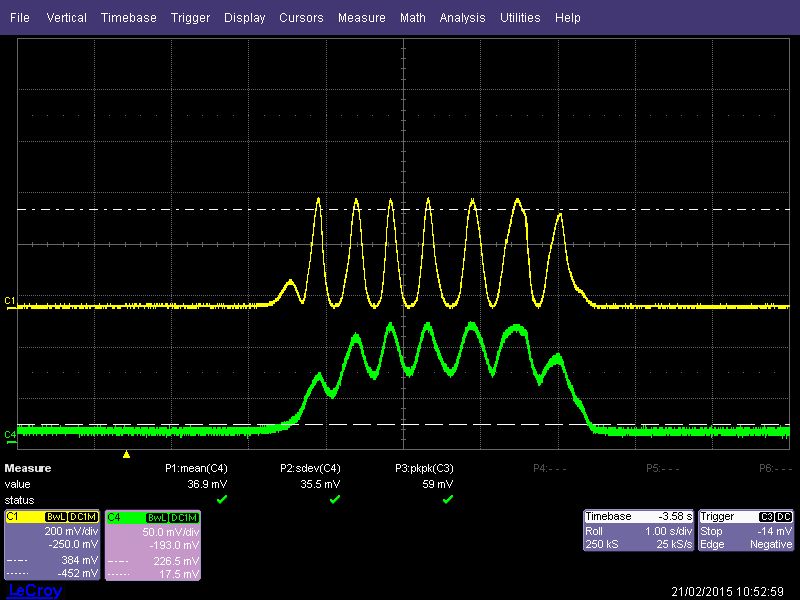
\includegraphics[width=\textwidth]{yscan.png}
    \caption{}
    \label{fig:yscan}
    \end{subfigure}
    \hfil
    \begin{subfigure}[b]{0.49\textwidth}
    \centering
    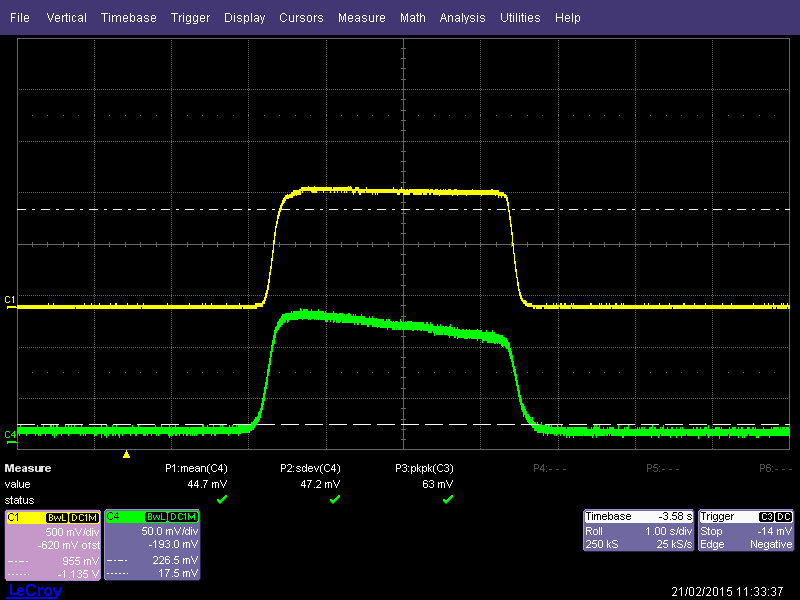
\includegraphics[width=\textwidth]{yscan_after.png}
    \caption{}
    \label{fig:yscan_after}
    \end{subfigure}
\caption{Screenshots of the oscilloscope display showing transmission and reflection curves as the laser beam is moved across the membrane. (a) Before fixing the tilt and (b) after fixing the tilt.}
\label{fig:mem_tilt}
\end{figure}

\subsection{Cavity alignment}
When the tilt is minimized we put in the top mirror and place a spring on top of it before enclosing it with the top sample holder piece. The screws are not screwed all the way in because we need to push around the top curved mirror to obtain a cavity. This is the so called ``pinhead procedure". It can be advantageous to go a wavelength with a relative low finesse to make life a bit easier, because lower finesse cavities have broader resonance and are therefore more likely to be spotted while scanning the laser wavelength. This trick is general when assembling cavities.

When a cavity has been realized we move to a high finesse wavelength (\SI{852}{\nano\meter}) and scan the wavelength until we see the transverse mode $TEM_{(00)}$ on the camera, see figure \ref{fig:beam_place}. We then maximize the transmission of this transverse mode, by scanning the laser frequency fast across the cavity resonance and optimizing the cavity response detected on the transmission detector.

\subsection{Illumination of membrane}
We use four LED's placed tightly together in a circle with a hole in the middle, allowing for the laser beam to pass through and put it in the beam path, just before the cavity, we can illuminate the membrane and roughly estimate our beam position on the membrane mode as shown in figure \ref{fig:beam_place}.

\begin{figure}[H]
\centering
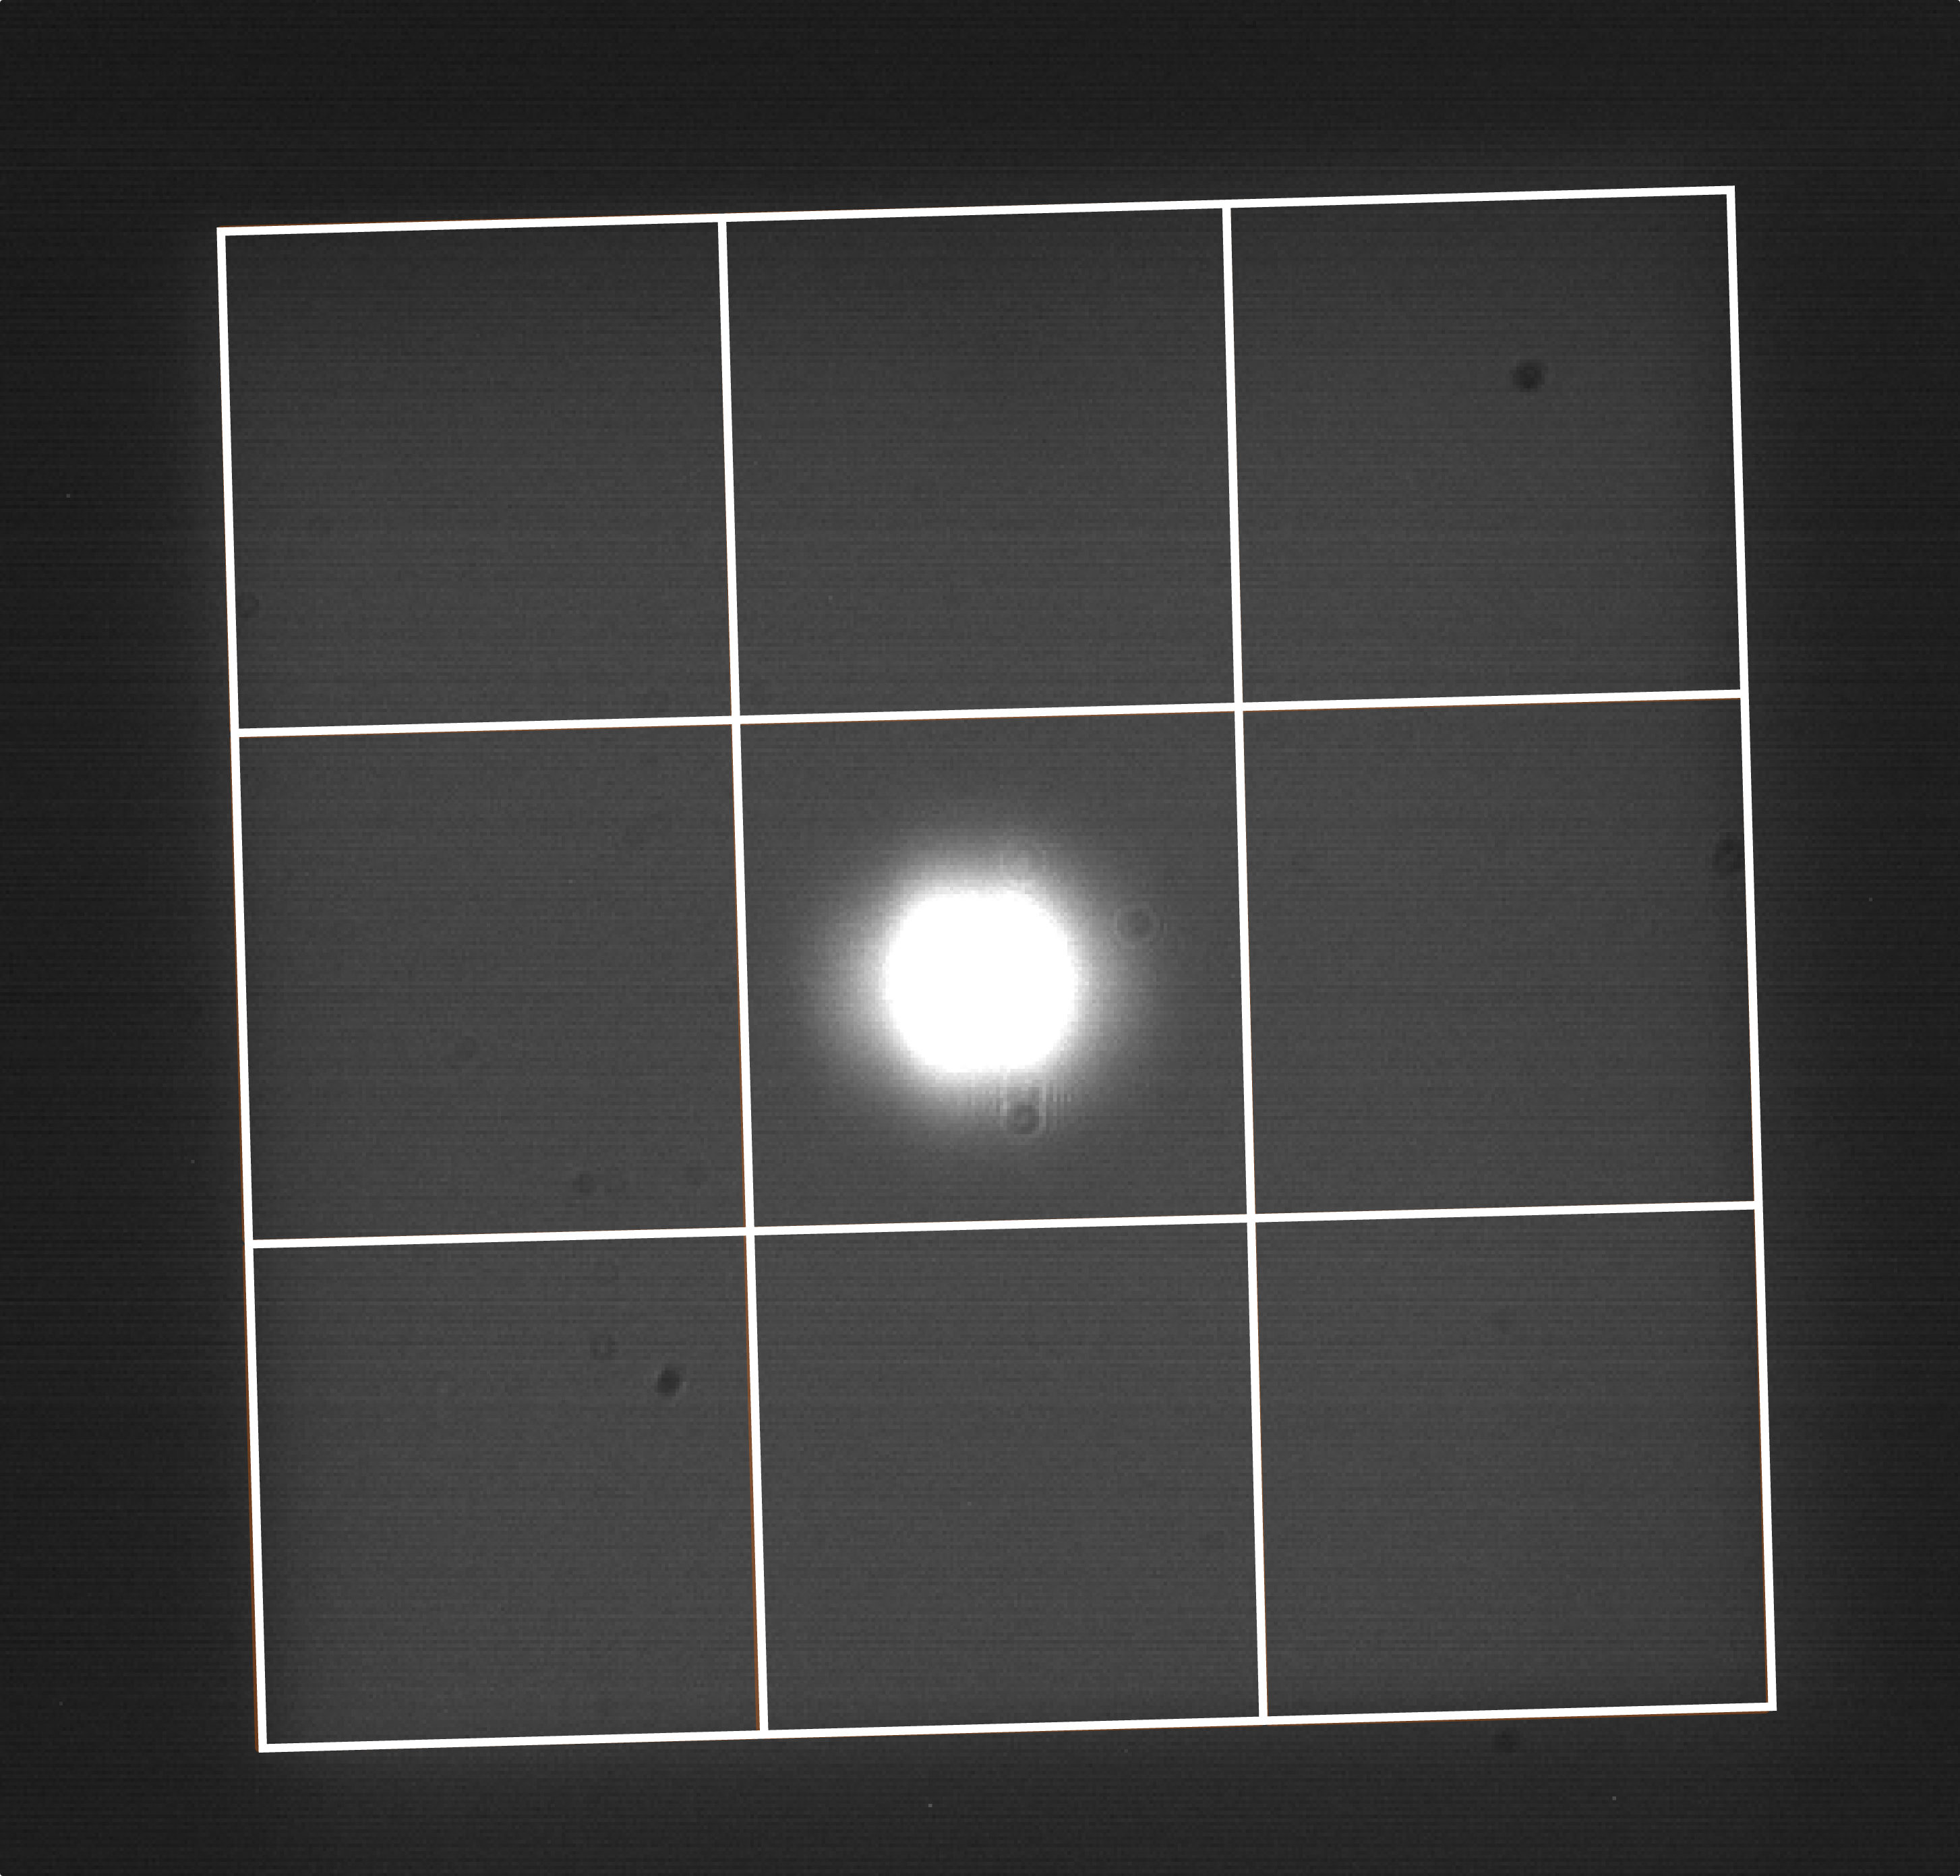
\includegraphics[scale=0.5]{membraneGrid.png}
\caption{Screenshot of the camera picture showing the illuminated membrane and the $TEM_{(00)}$ mode. The orange squares refers to the outline of the mechanical (3,3)-mode nodes.}
\label{fig:beam_place}
\end{figure}

A large overlap between the mechanical modes antinode and laser spot ensures a better coupling between the optical and mechanical degree of freedom.

\section{Cryostat}
Cryogenic temperatures for the setup are realized using a circulating helium system by Oxford Instruments\footnote{Oxford Instruments Microstat HiRes2}. The schematic overview is shown in figure \ref{fig:cryo_setup}.

\begin{figure}[H]
\centering
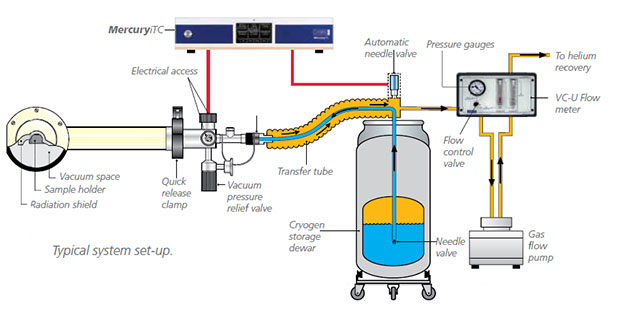
\includegraphics[scale=0.7]{cryostat.jpg}
\caption{An overview of the cryogenic setup. Picture taken from Oxford Intruments product webpage.}
\label{fig:cryo_setup}
\end{figure}

The cryostat is connected to a vacuum pump, such that a vacuum inside the cryostat can be achieved. We normally reach a vacuum of \SI{1e-6}{\milli\bar}, which is acceptable taking our cleaning and assemble procedure into account. Between the vacuum pump an the cryostat we have connected an extra tube enclosed in a heavy concrete block placed on vibration damping foam blocks, to prevent vibrations from the pump the travel to the cryostat. Even though the concrete block sounds and is low tech, it is quite crucial to the setup. Inside the cryostat a cold finger, is where we attach the sample holder. The cold finger is connected to the liquid helium by a transfer tube which is inserted into the dewar and then the cryostat. The transfer tube has two channels of flow. The one (inner) from the dewar to cold finger and the other (outer) from the cold finger to an exhaust. A gas pump and a flow meter are responsible for the continuous flow through the cycle. The amount of helium flow can be regulated by a needle valve on the transfer tube and or by a control valve connected to pressure gauge on the flow meter.

To measure the temperature inside the cryostat a temperature sensor is included in the cold finger. More temperature sensors could be added, for example in the sample holder close to the sample, but we ran out of sensors. The temperature can be stabilized by a heater. The cryostat's specified minimum temperature is around the temperature of liquid helium \SI{4.2}{\kelvin}.

\chapter{Experiment and results}

\section{Sideband cooling}
This section is a description of the experiment on how well our optomechanical membrane-in-the-middle system, at the current state, can cool the nanomechanical membrane's (3,3)-mode starting at cryogenic temperatures. The (3,3)-mode has shown high quality factors at room temperature and has promising optomechanical single-photon coupling strength. The complete experiment consist of four smaller sub-experiments. We will in detail describe these sub-experiments and show their results. We will start out by measuring the mechanical ringdown time by optical excitation, to confirm high quality factors at cryogenic temperatures, then we will characterize the membrane-in-the-middle system by making a cavity resonance modulation map and by measuring the linewidth of the cavity. After these initial characterization measurements we will do a (red) detuning series, where we try to lock the laser to the cavity at high input power and close to cavity resonance as possible. We record an optomechanical-induced-transparency spectrum and a regular spectrum while we slowly red detune away from cavity resonance, to obtain the mean phonon occupancy for the mechanical mode.

Before we go into the description of how the spectra were obtained, we make a hand waving argument of why we are able to detect the membrane fluctuations. First let us consider a bare cavity transform phase fluctuations into amplitude fluctuations. If we place a membrane inside such a cavity, then the membrane fluctuations cause phase modulation of the light, which then will be transformed into an amplitude fluctuation. The amplitude fluctuations of the light are picked up by a detector. The detector converts the power fluctuations into a small fluctuating current via the photoelectric effect, which is then converted into a fluctuating voltage. The voltage is what we at the end of the day see as our signal on the oscilloscope. All of these conversions are considered to be linear for small fluctuations. We can also from a simple cavity response consideration predict when an optomechanical cavity is most sensitive to small phase fluctuations, which is when we are detuned by half of the cavity linewidth, because the slope of the cavity response (derivative of Lorentzian) is the steepest at exactly this detuning.

\subsection{Mechanical ringdown measurement} \label{sec:q_fact}
We measure the quality factors of the membrane resonator in our setup, by moving to lower wavelengths (roughly \SI{730}{\nano\meter}). At this wavelength our cavity is so transmissive that  cavity enhanced radiation pressure effects can be neglected. We then optically excite the membrane using radiation pressure force. The optical excitation is done by switching to the alternative input (see figure \ref{fig:presetup}) and increasing the input power to roughly \SI{3}{\milli\watt}. The voltage sent to the AOD is modulated by using a TTL switch board. For this we use two signal generators. The first signal generator\footnote{Rohde \& Schwartz SMC100A} modulates the AOD voltage at the mechanical frequency and the second signal generator\footnote{HP 33120A} puts an overall modulation on top of the first signal, which is much slower than the mechanical frequency. Thus the alternative input consists of small bursts of excitation followed by a period where the AOD is not fed any voltage signal so we can detect a signal. For detection we have swapped transmission detector\footnote{Thorlabs PDA8}, because the other detector does not tolerate the high powers we need for excitation. The detector output is sent to a lock-in amplifier\footnote{Zurich Instruments HF2LI} and is here demodulated at the mechanical frequency from the first signal generator. We look for the narrow mechanical resonance by scanning the frequency of the first signal generator. When the mechanical resonance is found we slowly decrease the frequency of the second signal generator to accommodate for the ringdown time, i.e. detecting the actual signal and not interrupting it by yet another excitation burst. The ringdown time trace is then recorded on the oscilloscope. See figure \ref{fig:ringdown_trace} for an example trace.

\begin{figure}[h]
\centering
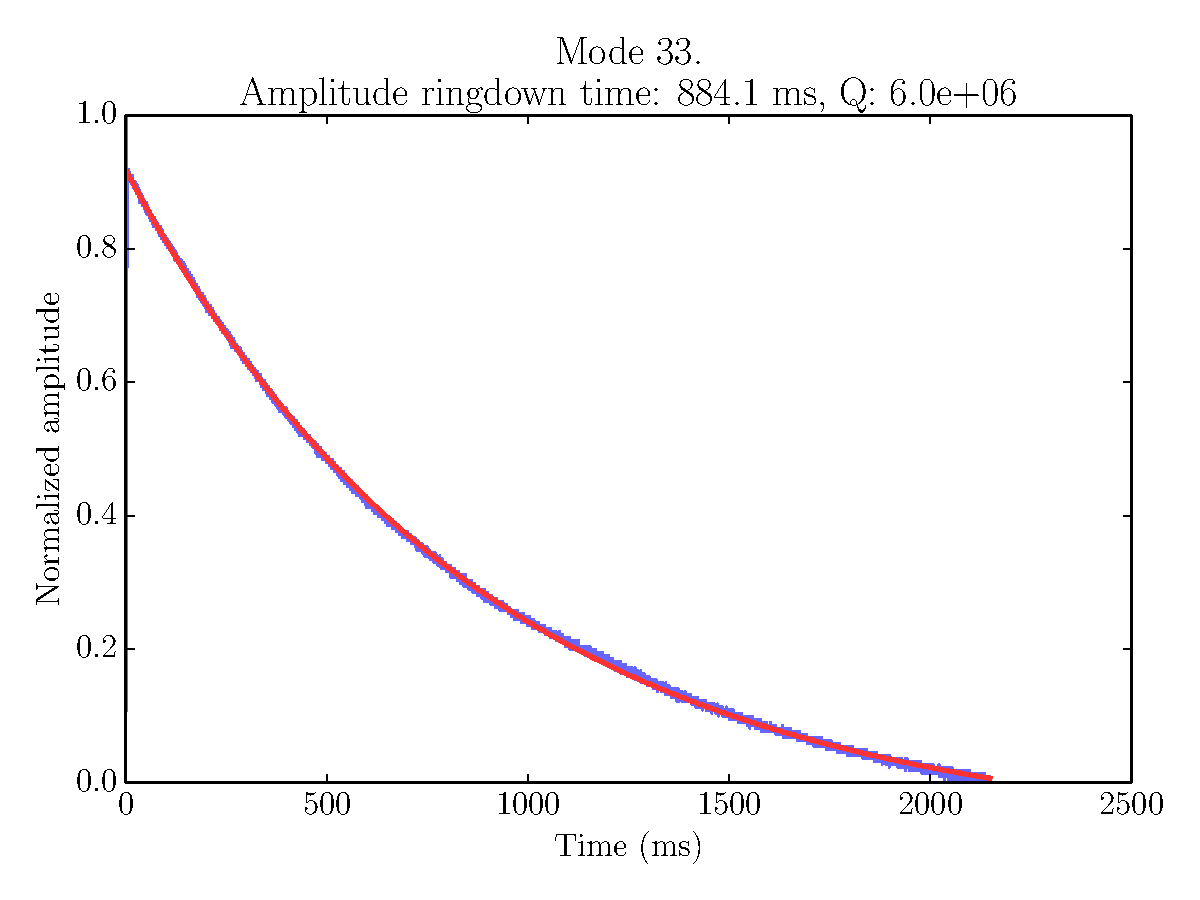
\includegraphics[scale=0.8]{analysis/ringdown_33_4k.pdf}
\caption{Ringdown time trace recorded at cryogenic temperatures.}
\label{fig:ringdown_trace}
\end{figure}

From the eight recorded ringdown traces of the (3,3)-mode at cryogenic temperature we get a quality factor of

\begin{equation}
Q = (6.0 \pm 0.5) \times 10^6,
\end{equation}
\noindent
where the uncertainty is the standard deviation of the measured values. We confirm that the quality factor of the mechanical mode is in fact high and therefore a good prospect for optomechanical induced cooling experiments. The mechanical damping rate is $\Gamma_m/2\pi \approx $ \SI{0.4}{\hertz}.

The use of a secondary signal generator could have been avoided by using a secondary laser beam to detect the signal. Our procedure makes things more complicated and tedious. Because the mechanical resonance is jumping around on the scale of a few \SI{}{\hertz}, while the linewidth is often also \SI{}{\hertz} scale. This makes tracking the resonance and adjusting the timescales a bit difficult.

\subsection{Characterization of the MIM system} \label{sec:char_mim}
To achieve as high optomechanical coupling as possible it is important to know, where the membrane is in the standing wave inside the cavity. Another important measure is the unmodulated free spectral range denoted by $FSR_0$. This measurement has to be made at cryogenic temperature, as the cavity dimensions are not stable under \SI{300}{\kelvin} $\rightarrow$ \SI{4}{\kelvin} transition, which shifts the cavity resonances.

We obtain these quantities by searching for cavity resonances in the relevant wavelength region, which in our case is \SI{852}{\nano\meter}. We identify the cavity $TEM_{00}$ resonances by use of the camera. We note down the wavelength of the resonance and move on to find the next cavity resonance. Eight resonances is sufficient, but for higher resolution twelve or higher is recommended\footnote{At the same time we do not want to waste precious helium.}. We ended up noting down twelve resonances ranging from \SIrange{850.8}{852.9}{\nano\meter}. We then convert the wavelengths to frequencies and perform a linear fit of cavity resonance frequency as a function of resonance number. The slope of the fit is our $FSR_0 \approx$ \SI{85.0}{\giga\hertz}, corresponding to a cavity length of $L \approx$ \SI{1.77}{\milli\meter}.

We now want to use the transfer matrix model to find at which cavity resonance is the membrane placed closest to a node of the standing cavity wave. To find this point, we subtract the fitted line from the cavity resonance frequencies and assume that the highest frequency value is placed at a node, i.e. zero cavity resonance modulation as in our prediceted model from section \ref{sec:trans_matrix}, which is justified as the membrane inside the cavity can only make cavity length $L$ longer. By using this method we are constantly underestimating the resonance modulation caused by the membrane in the cavity, but this is a small systematic error caused by the relative low resolution, which we do care about since it is just an offset.

To find the membrane position away from the end mirror denoted $\Delta x$ we fit the following model \eqref{eq:resonance_var} to our data. We expect a periodic behaviour modulation in $k$ with period $T_k = \pi/\Delta x$. We ``fold back" the series into the k-range $[0, \pi/\Delta x]$ by sending $k \rightarrow \mathrm{mod}_{\pi}(k\Delta x)$. We end up with the following figure (see \ref{fig:2kz}), showing the cavity resonance frequency modulation as a function of $\mathrm{mod}_{\pi}(k\Delta x)$.

\begin{figure}[H]
\centering
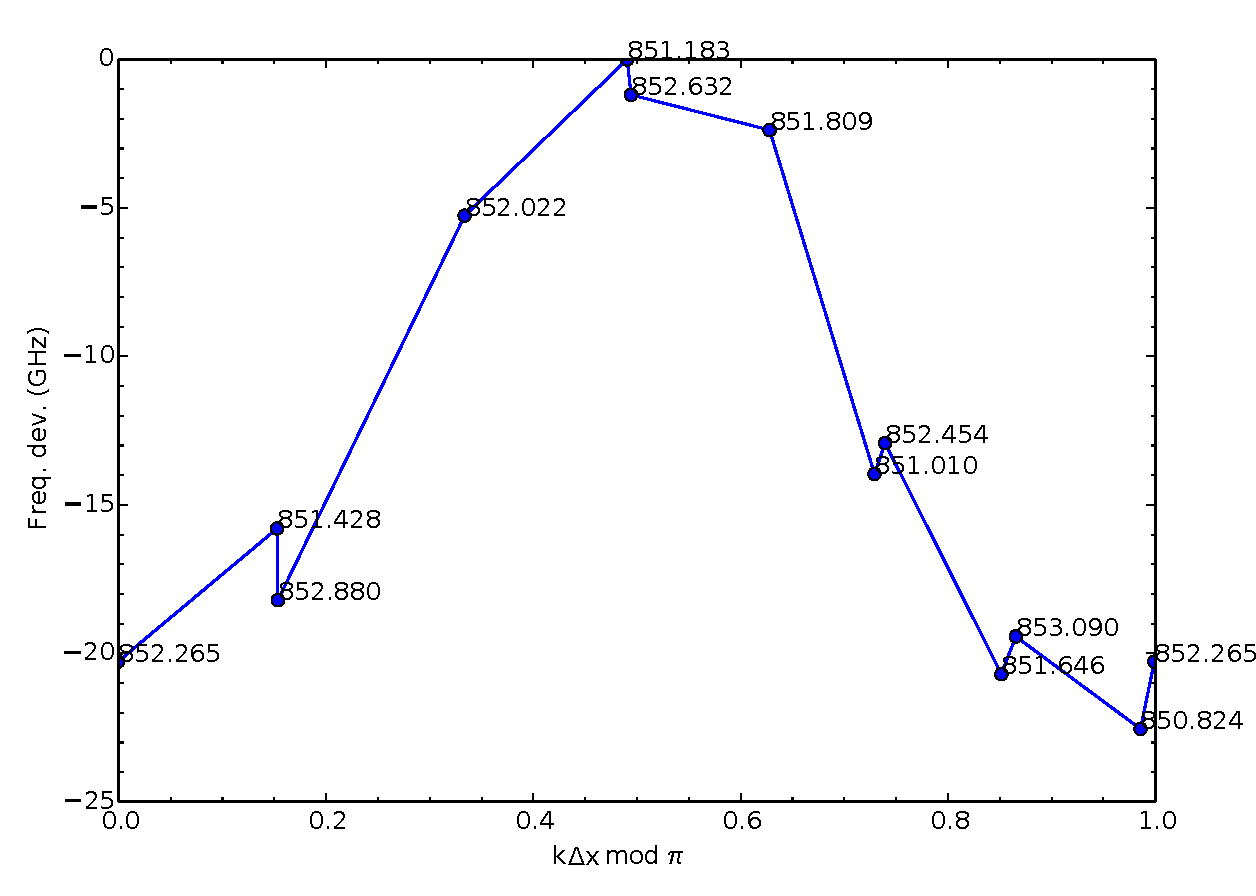
\includegraphics[scale=0.75]{analysis/2kz_mod.pdf}
\caption{Periodicity of the cavity resonance frequency modulation.}
\label{fig:2kz}
\end{figure}

We can now choose a cavity resonance with a high coupling from one of the two slopes of figure \ref{fig:2kz}. But it turns out that experimentally we cannot lock to the cavity resonances on the positive slope, due to what we expect to be a thermal instability. The instability is thought to arise from an asymmetry in the membrane chip geometry, which make it always protrude a little in one direction, causing heating to either push the protrusion towards an unstable region or a stable region depending on position in the standing wave. We can simple state that one slope is stable, while the other is not. We choose our stable cavity resonance coupling point to be at \SI{852.454}{\nano\meter}.

We measure the linewidth for this particular cavity resonance, by scanning the laser frequency across the resonance, while having EOM generating sidebands to calibrate the time axis from the oscilloscope to frequency.

\begin{figure}[H]
\centering
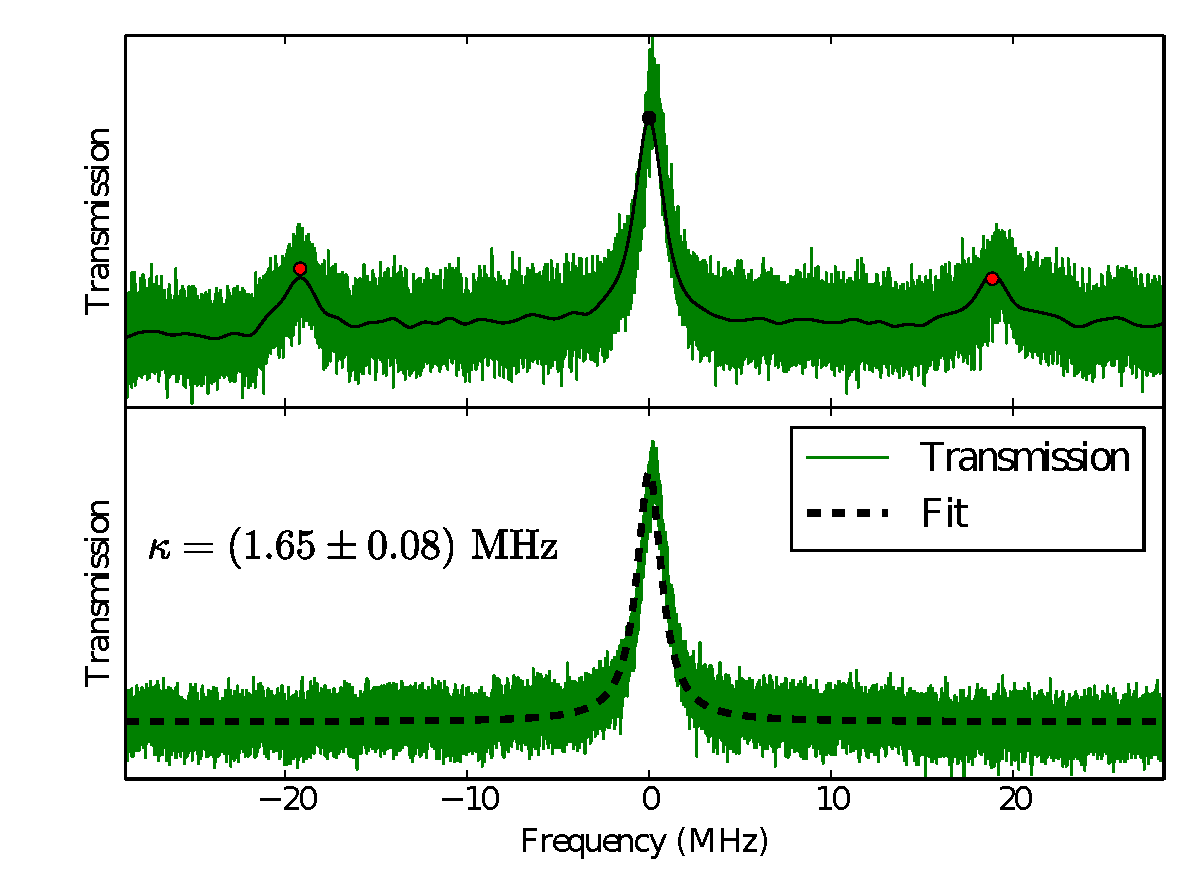
\includegraphics[scale=0.75]{analysis/cav_linewidth.pdf}
\caption{Example of a cavity linewidth measurement. Upper part of the figure show the time trace with sidebands and the lower part show the calibrated to frequency cavity response.}
\label{fig:2kz_cav_lw}
\end{figure}
\noindent
From the three consecutive measured linewidth we get an average of $(1.60 \pm 0.06)$ \SI{}{\mega\hertz}. The increase in cavity linewidth compared to the bare cavity of \SI{0.5}{\mega\hertz} can be assigned to finesse modulation seen from the transfer matrix model \cite{Wilson2011} and not from additional external losses caused by membrane tilt or poor alignment.

\subsection{Optomechanical induced transparency} \label{sec:exp_omit}
For the detuning series we initially want to lock the laser to the cavity. The lock is set up by using the transmission DC signal as our error signal with an adjustable offset, which is sent through our feedback loop to the laser. This kind of lock is advantageous, because it easy to set up, works well when far detuned and can easily stay locked for large periods of time, for example while recording multiple spectra. A disadvantage is that this lock, compared to a PDH-lock, is sensitive to fluctuations in input power. We lock the laser at an input power of \SI{1}{\milli\watt}. We detune away from cavity resonance simple by changing our locking offset point. This is seen as a decrease in DC level on the oscilloscope, we write down the DC level for every detuning.

The optomechanical induced transparency is performed by using the EOM to generate the weak probe field with the output source from vector network analyzer\footnote{Rohde \& Schwartz ZNB20}, which is then sweept in frequency from \SIrange{0}{10}{\mega\hertz}, i.e. across the cavity response. The sidebands are generated with a source power of \SI{-15}{\deci\bel\milli} and the transmission detector's AC signal is fed as the input to vector network analyzer, but is attenuated by \SI{13}{\deci\bel} to avoid overloading. We record the spectra of the driven cavity response for different detunings from \SI{100}{\kilo\hertz} to \SI{10}{\mega\hertz} with 50 k samples, see an example of such a spectrum in figure \ref{fig:omit_cavity}.

\begin{figure}[H]
\centering
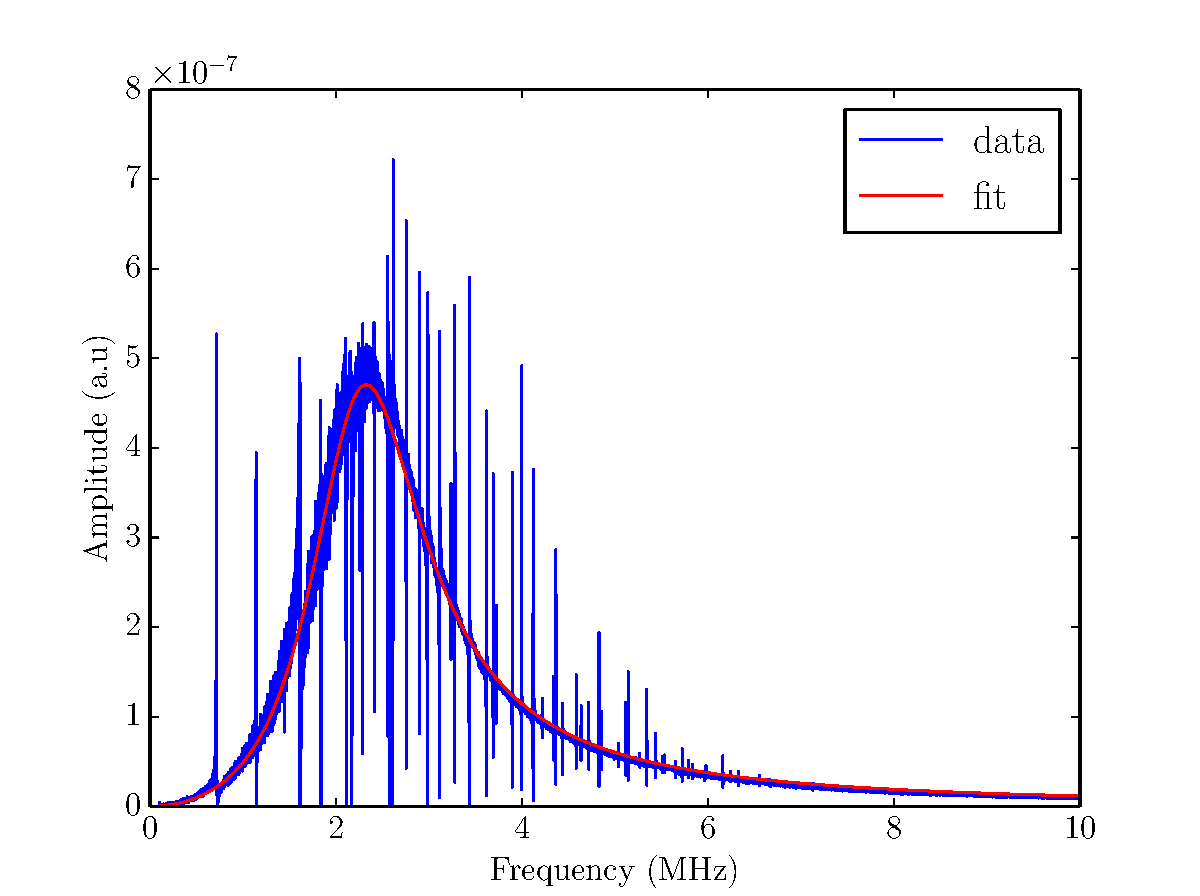
\includegraphics[scale=0.8]{analysis/omit_fit_detuning_new.pdf}
\caption{Example of driven cavity response spetrum from a optomechanical induced transparency measurement. As a rough rule of thumb the cavity response peak frequency is equivalent to the detuning.}
\label{fig:omit_cavity}
\end{figure}

We can obtain the detuning $\bar{\Delta}$ and the cavity linewidth by applying the OMIT model to the normalised response curve. The reasoning behind using the normalised data instead of the raw data, is that amplitude and detuning are not independent, i.e. two different set of values can produce the same curve. Futhermore we set the coupling and mechanical linewidth to zero, so that we only fit to the broad cavity response as shown in figure \ref{fig:omit_cavity}. From the fitting we get the detuning as a function of DC voltage level from the detector see figure \ref{fig:omit_detuning}.

\begin{figure}[H]
\centering
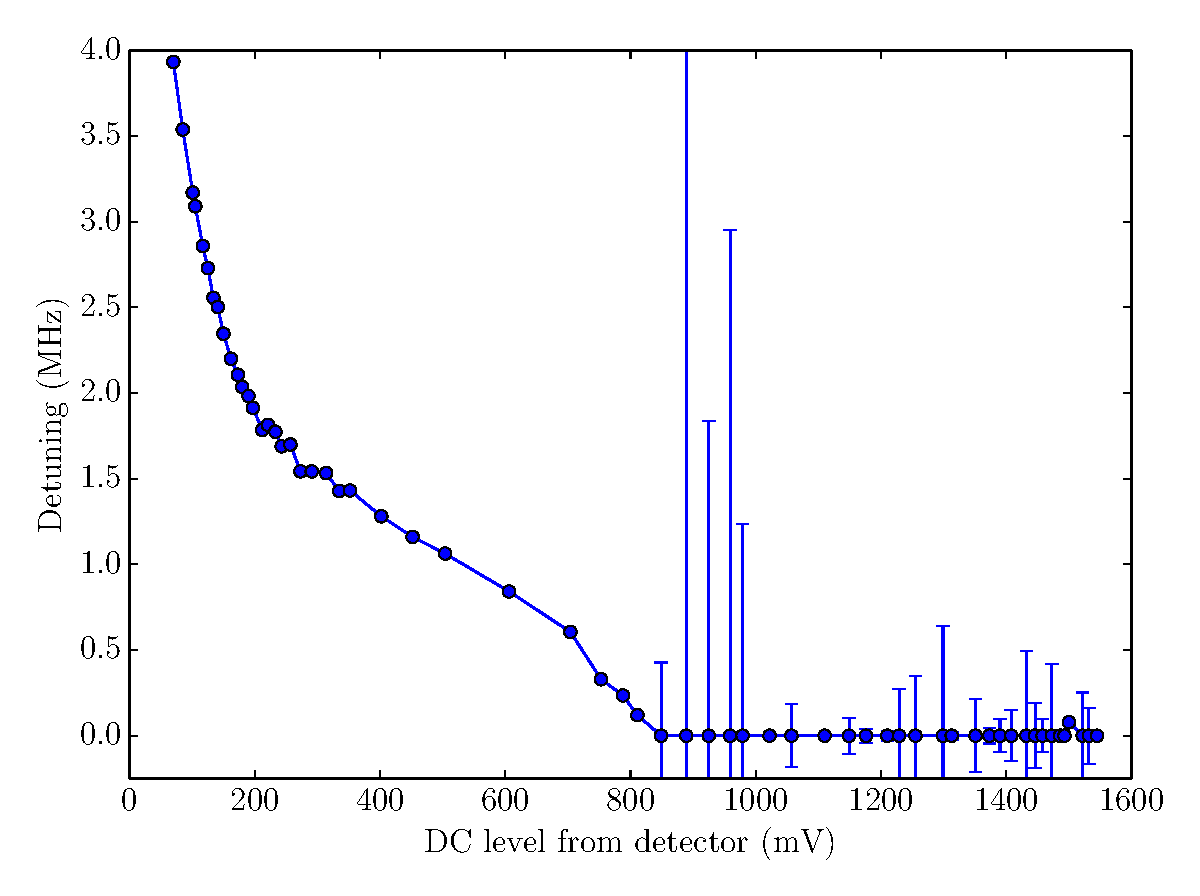
\includegraphics[scale=0.7]{analysis/detuning_vs_DC.pdf}
\caption{The obtained detunings from fitting, showing the detunings for different detector voltages. The uncertainties are the standard deviations from the fit.}
\label{fig:omit_detuning}
\end{figure}

We see from the figure \ref{fig:omit_detuning} that the fit is untrustworthy for small detunings, i.e. detunings lower than \SI{0.5}{\mega\hertz}. Therefore detunings lower than \SI{0.5}{\mega\hertz} will be discarded and that is also acceptable, since we are really only interested in what happens at detunings close to the mechanical frequency, i.e. \SI{2.17}{\mega\hertz} for maximum cooling effects. This is a good time to point out that we do not know our detuning precisely while experimenting, unless we take optomechanical induced transparency traces. We could of course do rough estimates from the Lorentzian cavity line shape, if we know our cavity linewidth. Apropos linewidth we also get this parameter from our fit, see figure \ref{fig:omit_cavity_lw}.

\begin{figure}[H]
\centering
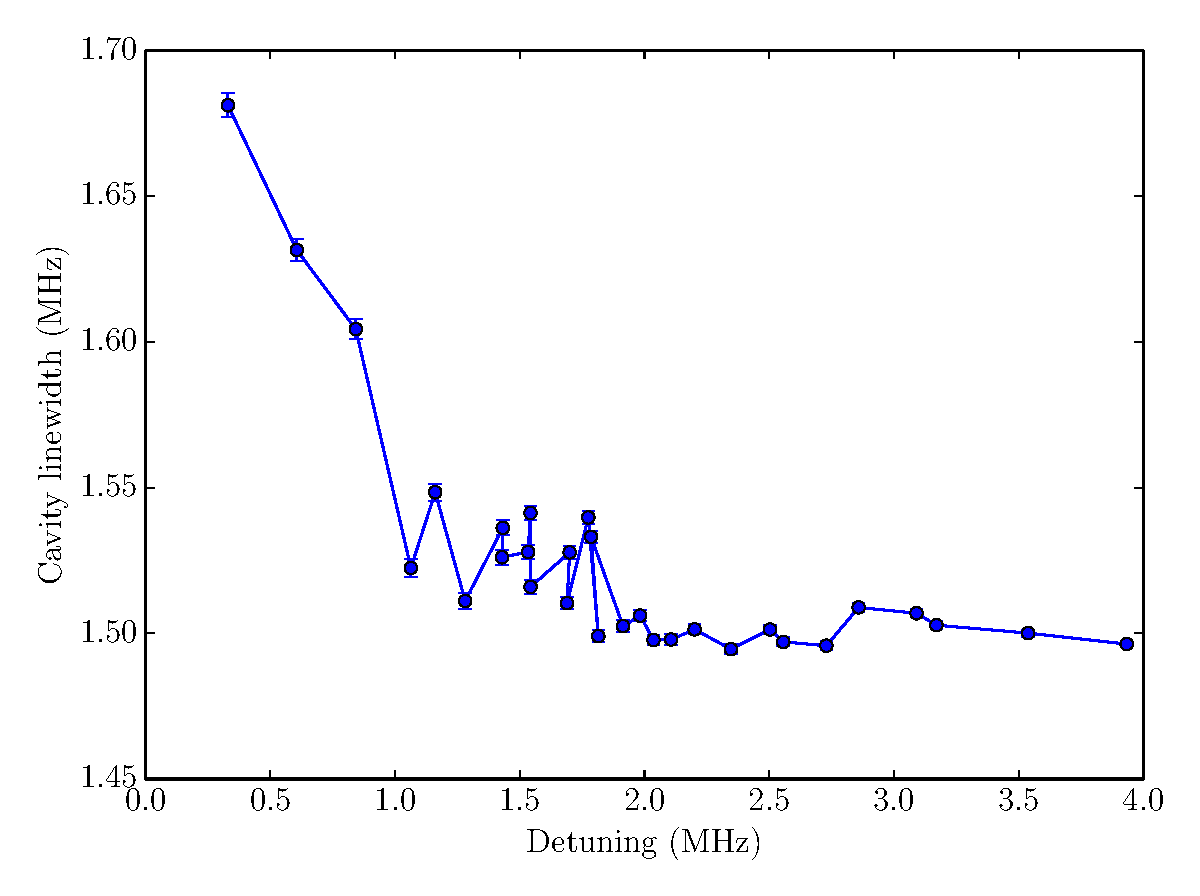
\includegraphics[scale=0.7]{analysis/cavity_lw_vs_detuning_new.pdf}
\caption{Extracted cavity linewidth from the fit to the cavity response. The uncertainties are the standard deviations from the fit.}
\label{fig:omit_cavity_lw}
\end{figure}

We see in figure \ref{fig:omit_cavity_lw} that the cavity linewidth stabilizes for higher detunings. From the optomechanical induced transparency model we get a cavity linewidth of $(1.54 \pm 0.05)$ \SI{}{\mega\hertz}. This result fits well with the independent measured linewidth from section \ref{sec:char_mim}, which is a nice sanity check of our cavity response fit procedure. The rapid increase in cavity linewidth for small detunings is a fitting artifact.

We now turn to fit our model for optomechanical induced transparency at the mechanical frequency (\SI{2.17}{\mega\hertz}) of the (3,3)-mode, i.e. obtaining the light enhanced optomechanical coupling $g = g_0\sqrt{\bar{n}_{cav}}$, where $g_0$ is the single-photon coupling strength defined as $g_0 = Gx_{zpf}$. We perform the fit by choosing a suitable range around the mechanical resonance as seen in figure \ref{fig:omit_g}. The fit parameter $g$ is the width of the dip, while the center of it is the mechanical resonance frequency. The mechanical linewidth is assumed to be zero in our applied model, this is a good assumption because the effective mechanical linewidth will be dominated by the optical induced linewidth.

\begin{figure}[H]
\centering
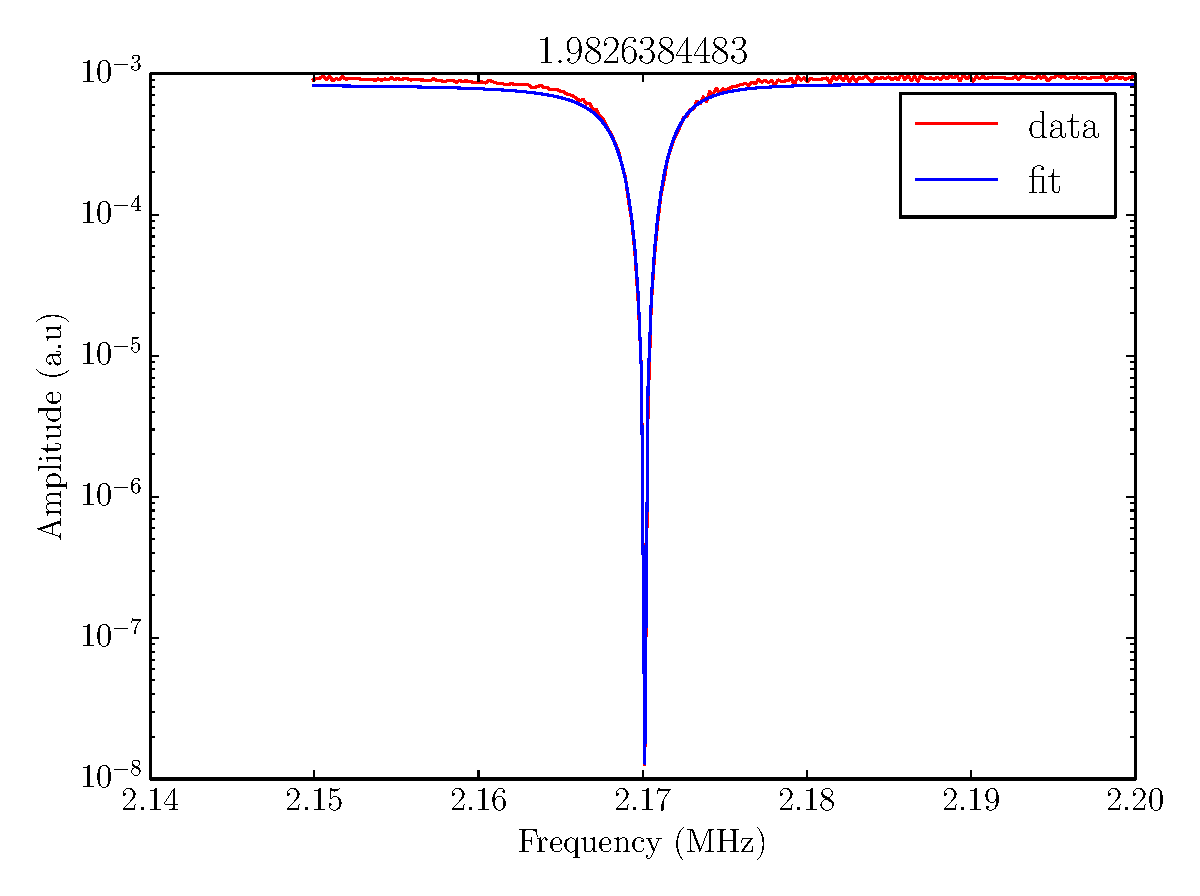
\includegraphics[scale=0.7]{analysis/omit_fit_dip_zoom.pdf}
\caption{Optomechanical induced tranparency. The figure title is the detuning in MHz.}
\label{fig:omit_g}
\end{figure}

We can gain a lot of insight from the fitted parameter $g$, for example $g_0$. If we can work out the intra-cavity photon number, we can obtain $g_0$, which is important for calibrating a spectrum. We can obtain the intra-cavity photon number by using equation \eqref{eq:cav_circ_pwr} and converting the recorded detector DC voltage into an optical power.

\begin{figure}[H]
\centering
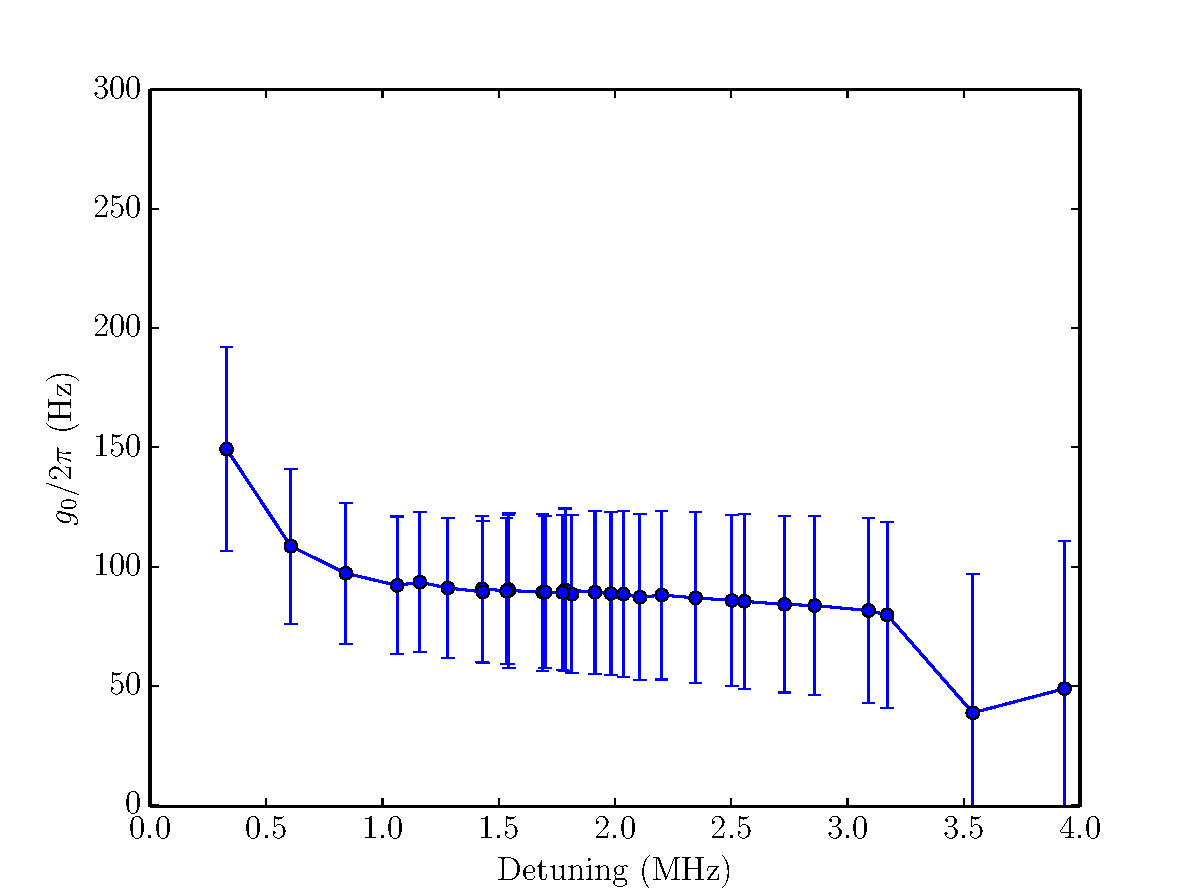
\includegraphics[scale=0.8]{analysis/omit_g0.pdf}
\caption{Single-photon coupling strength as a function of detuning. The errorbars are given by the standard deviation from the fitted $g$.}
\label{fig:omit_fit_g0}
\end{figure}

We get a single-photon coupling strength of $g_0/2\pi = (88.2 \pm 16.8)$ \SI{}{\hertz}. This value of $g_0/2\pi$ sounds reasonable, because a rough estimate of the expected single-photon coupling strength for our parameter set is given by $Gx_{zpf}$. The zero-point fluctuation, using equation \eqref{eq:xzpf}, for the (3,3)-mode is \SI{0.6}{\femto\meter} and if we approximately set $G$ for a Fabry-Perot cavity by $\frac{\omega_c}{L}$, then we should expect \SI{122}{\hertz}. A reduction of $g_0$ is expected from the overlap integral between the beam spot and mechanical mode shape and from the low reflectivity of the membrane \cite{Wilson2011}.

We can also extract the expected optically induced damping $\Gamma_{opt}$ from the cavity resonance by using $g$ and equation \eqref{eq:gamma_opt}. As an approximation we will assume $\Gamma_{opt} \approx \Gamma_{eff}$, since the mechanical linewidth is on the order \SI{}{\hertz} and the optically induced linewidth is on the order \SI{}{\kilo\hertz}. This estimate is shown in figure \ref{fig:omit_fit_gamma_opt}.

\begin{figure}[H]
\centering
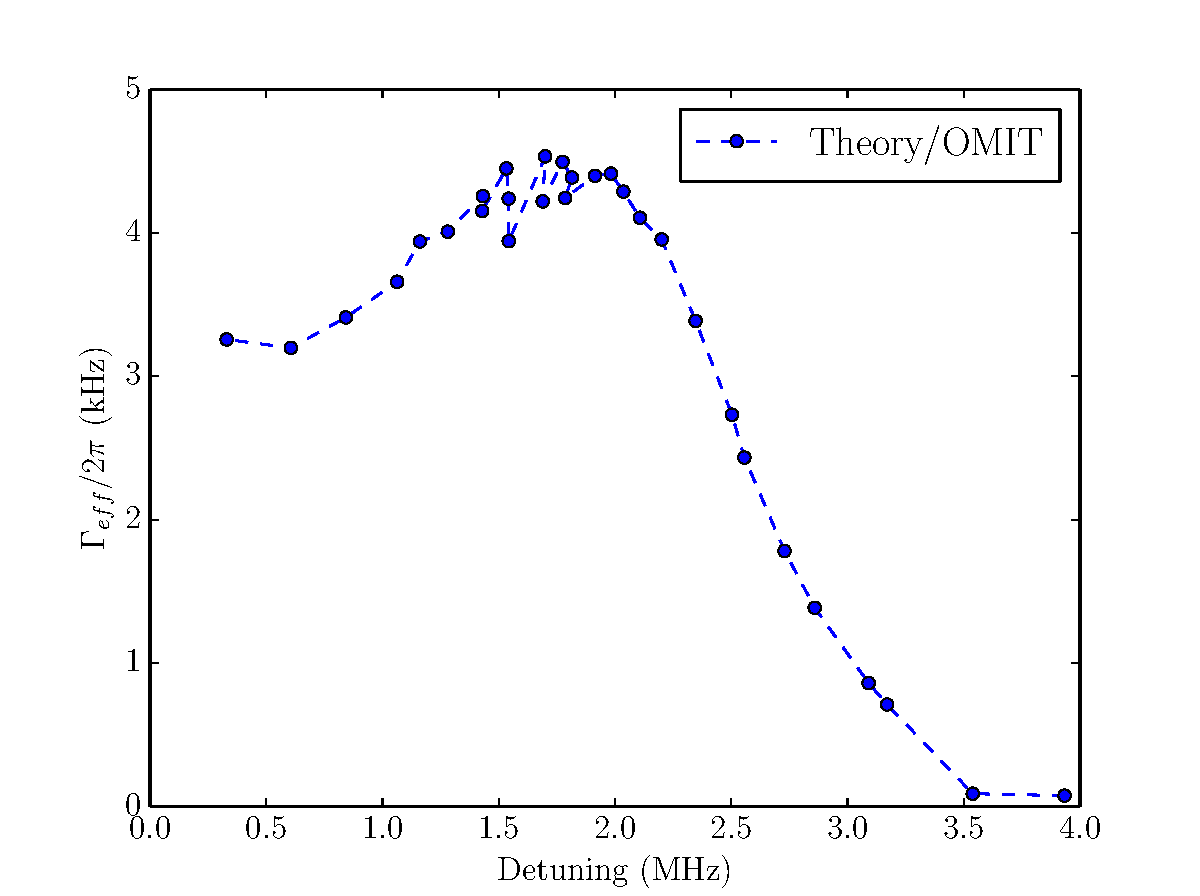
\includegraphics[scale=0.8]{analysis/gamma_opt_vs_detuning.pdf}
\caption{The expected effective mechanical linewidth as a function of detuning.}
\label{fig:omit_fit_gamma_opt}
\end{figure}

We do not know the temperature of the bath that we couple to, so estimating a mean phonon occupancy from the effective damping would not make much sense. The bath temperature can be extracted from the simultaneously recorded spectrum, with a calibraiton peak, of the intensity fluctuations from the cavity caused by the membrane fluctuations, for each individual detuning.

\subsection{Spectrum} \label{sec:ex_spec}
We now turn to the experiment of recording the spectra of the fluctuating membrane, which later on can be calibrated. From the calibrated spectrum we can extract the effective mechanical mode temperature by integrating the mechanical resonance as shown in section \ref{sec:xrms}. We record the spectra from the AC output from the detector, which is \SI{5}{\mega\hertz} low-pass\footnote{Mini-Circuit NLP-5+} filtered twice to avoid aliasing, before sending the signal to a data acquisition-card\footnote{Adlink PCI-9846H}. To generate a calibration tone the EOM is driven by a signal generator\footnote{Rohde \& Schwartz SMC110A} at a frequency of \SI{2.185}{\mega\hertz} and a power of \SI{-56}{\deci\bel\milli}. The spectra is recorded averaging 50 times with a sample rate of \SI{10}{\mega} and a resolution bandwidth of \SI{10}{\hertz} for each detuning, after the OMIT trace while maintaining the lock.

The calibration of the spectra is done according to the routine sketched in \cite{gorodetsky2010}. We calibrate the spectra using the scaling factor

\begin{equation}
F_{calib} = \frac{\beta^2f_{mod}^2}{A_{calib}}\left(\frac{x_{zpf}}{g_0}\right)^2,
\end{equation}
\noindent
where $f_{mod}$ is EOM modulation frequency, $A_{calib}$ is the area under the calibration tone and $\beta$ is magnitude of phase modulation in the light ($\beta = \sqrt{P_{eom}R(\pi/V_{\pi})^2}$) as in \cite{black2001}. Our $V_{\pi}$ is measured to be \SI{2.09}{\volt}. We use the $g_0$ found from the OMIT fit seen in figure \ref{fig:omit_fit_g0}. The new spectra we get from the calibration procedure around the mechanical resonance are shown in figure \ref{fig:spec_calib} for a selection of relevant detunings.

\begin{figure}[H]
\centering
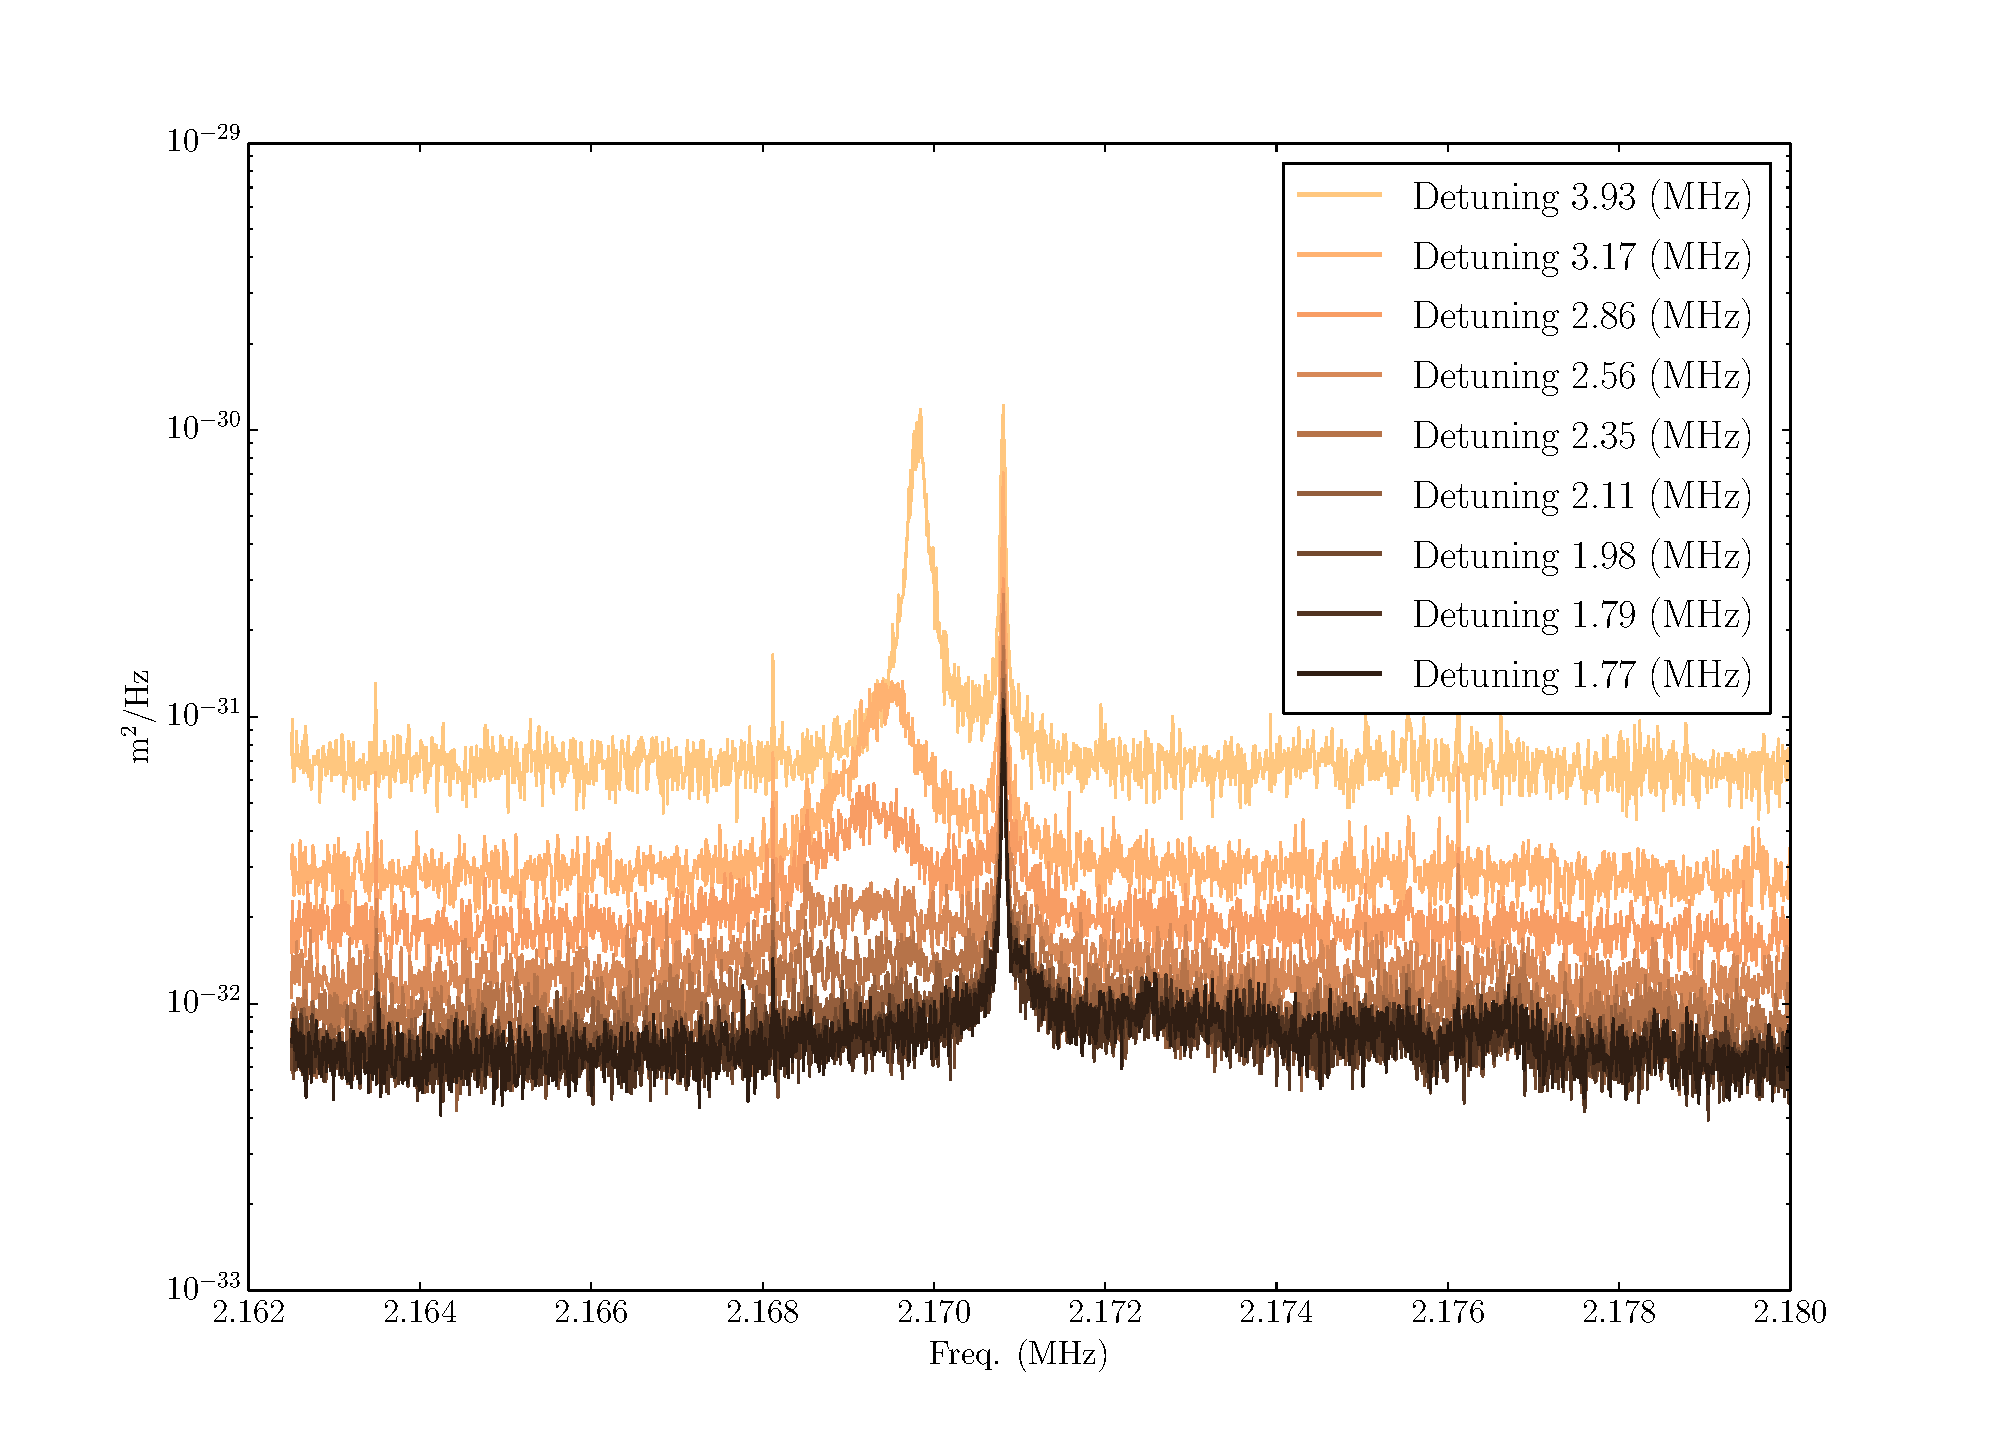
\includegraphics[scale=0.45]{analysis/cal_spec_newest0.pdf}
\caption{Broadening of the mechanical resonance in calibrated spectra as the detuning is changed towards optimal condition for cooling. The large peak at \SI{2.171}{\mega\hertz} is unfortunately unwanted noise.}
\label{fig:spec_calib}
\end{figure}

We see in the figure above that the mechanical peak gets broadened as expected from theory as we detune towards the optimal condition for sideband cooling. The mechanical resonance gets hard to distinguish form noise, but nevertheless the signal-to-noise ratio never drops below unity for the full detuning series. We are quite unlucky because a noise peak, which was not present in preliminary test, is showing right on top of the broadened resonance. The noise is unfortunate, but we can work around it, when fitting a Lorentzian to mechanical peak for finding the effective damping, by either fitting a double-Lorentzian to the noise and mechanical peak or simply by cutting out the unwanted noise, since it is static as seen in figure \ref{fig:spec_calib}. We did both and they yielded roughly the same result, but the latter was more invariant/robust to changes like fitting range, i.e. the number of points fitted. A plot showing the fitted effective damping from the spectra compared to the effective damping obtained from the OMIT fit can be seen in figure \ref{fig:spec_eff_damp}.

\begin{figure}[H]
\centering
\includegraphics[scale=0.7]{analysis/eff_damp_newest.pdf}
\caption{Effective damping from the Lorentzian fit of the mechanical resonance compared with the prediction made from the OMIT fit.}
\label{fig:spec_eff_damp}
\end{figure}

The OMIT fit seems to consistently underestimate the effective broadening of the mechanical mode, for detunings near the mechanical resonance, but they follow the same tendency and the agreement between model and data is good. From the amplitude of the Lorentzian fit we get the calibrated area beneath the mechanical mode. The area determines the effective temperature of mechanical mode by \eqref{eq:t_eff}. Using the effective temperatures and Bose-Einstein distribution, we calculate the mean phonon occupancy $\bar{n}_{phonon} = \left[e^{\hbar\Omega_m/k_BT_{eff}} - 1\right]^{-1}$. We shown the mean phonon occupation number as function of detuning in figure \ref{fig:phonon_occ}.

\begin{figure}[H]
\centering
\includegraphics[scale=0.7]{analysis/phono_occ.pdf}
\caption{The extrapolated mean phonon occupancy of the mechanical (3,3)-mode.}
\label{fig:phonon_occ}
\end{figure}

The minimum mean phonon occupancy from the recorded spectra is $\bar{n}_{phonon}^{min} \approx 27\substack{+11 \\ -7}$. The errors is a combination of the easy accessible errors from the fitted $g_0$ and the error on the fitted area. We have not included more complex uncertainties, due to time constrains, from $V_{\pi}$, the calculated cavity photon number $\bar{n}_{cav}$ and corrections from the transduction function of the signal sent to the EOM.

\chapter{Concluding remarks and outlook}
We set out to rigorously test the cooling performance of our optomechanical membrane-in-the-middle system, showing with some precision that we can cool a mechanical mode down to a mean phonon occupancy of $\bar{n}_{phonon}^{min} \approx 27\substack{+11 \\ -7}$, corrosponding to an effective temperature of $T_{eff} \approx$\SI{3}{\milli\kelvin}. While not being in the ground state we can still appreciate the low phonon occupancy and the extremely low temperature. We can for example calculate the probability of being in the ground state $P_{n = 0} \approx 0.04$ given our current occupancy \cite{gerry2005}. We are actually in the ground state 4\% of the time. From equation \eqref{eq:nf} using our phonon occupancy we can extract the bath temperature we couple to, or in other words how well we thermalize the membrane through the sample holder. The bath temperature is found to be unexpectedly high, yielding $T_{bath} \approx$ \SI{43}{\kelvin}. This is unexpected since the cold finger is measured to be \SI{4}{\kelvin} (using the built-in temperature sensor in the cryostat) and at least in theory our sample holder should perform reasonably well. We have also from initial tests of thermalization seen indications of a membrane bath temperature of roughly \SI{10}{\kelvin} to \SI{30}{\kelvin}. Nonetheless, we can only draw two conclusions from the extracted bath temperature, either our sample holder do not thermalize the membrane or our spectrum is calibrated wrong and therefore estimates the phonon occupancy to be to high. Looking at the mentioned not included errors from the calibration process at the end of section \ref{sec:ex_spec}, we wrote that we neglected the corrections from the transduction function of the signal sent to the EOM. What lies behind the reasoning for excluding this is that the electronic line from the source to the EOM is unknown. We think that we had two power splitters, but we do not know which. Therefore, we assumed the osses to be \SI{6}{dB} and this could very well be a wrong assumption. The given EOM power in this work is the least generous for the phonon occupancy. If the power sent to the EOM was lower it would in fact correspond to a lower phonon number. The other neglected uncertainty is the mean intra-cavity photon number calculated from the detector's DC level. The model in \eqref{eq:cav_circ_pwr} is too simple to use and should have included a correction factor according from the transfer matrix model, because of the two sub-cavities not containing the same number of photons depending on the membrane position. We do not know in which direction it will shift the phonon occupancy and these considerations are therefore not included in this work.

As a final remark we will try to estimate weather or not the ground state is within reach for our setup. A parameter we know can be improved is the mechanical quality factor, as quality factors above ten million have been reached for some of our samples. This improvement would decrease the final phonon occupancy roughly a factor of two. If we trust the measured minimum phonon occupancy, we know that the main hindrance of reaching the ground state is the thermalization issue\footnote{A new improved generation of the sample holder has been machined and is now already installed in the lab.}. If thermalization can be improved by a factor of five, the future would look very bright. It is of course also possible to look for other mechanical modes with different couplings and thermal occupations. It thus seems that the ground state is indeed within reach.

\chapter{Additional projects}
Work done, but not included in the thesis.

\begin{itemize}
\item Setting up a diode laser for optical excitation of membrane modes.
\item Attempted squeezing of light.
\item Designing a next generation piezo-compatible sample holder.
\item Building a detector with high quantum efficiency for squeezing.
\end{itemize}

\appendix
\chapter{Bare cavity free spectral range} \label{sec:bare_fsr}
\begin{figure}[H]
\centering
\includegraphics[scale=0.7]{FSR_bare_cav.pdf}
\caption{Bare cavity resonances and a fit to determine the FSR.}
\label{fig:FSR_bare_cavity}
\end{figure}

\chapter{Relative intensity noise of the laser} \label{sec:rin}
\begin{figure}[H]
\centering
\includegraphics[scale=0.5]{solstis_rin.pdf}
\caption{The Ti:Sapph's relative intensity noise specifications, measured by MSquared.}
\label{fig:solstis_rin}
\end{figure}


\listoffigures

\listoftables

\printbibliography

\end{document}